\documentclass[
	language=en    ,
	layout=twoside ,
	titlepage=true ,
	preamble=false ,
	draftmode=false ,
]{sbmthesis}
\setlength\headheight{30pt} % required, do not delete

% \hyphenation{
%     % In some special cases LaTeX is unable to correctly hyphenate a term. Thus 		you have to define a custom hypenation rule here using minus signs. This is 		the case when a term overlaps with the page margins. Separate multiple 				entries with white space.
%     % Examples: Doppel-kupplungs-ge-triebe Kupp-lungs-schlupf-reg-ler
% }

\usepackage{amssymb}
\usepackage{amsmath}

% +-----------------------+
% | Start of the document |
% +-----------------------+
\begin{document}
    \preliminaries

    % +----------------------------+
    % | Include your chapters here |
    % +----------------------------+
    
    \chapter{Introduction}
\label{ch:Introduction}
To establish the foundation for this thesis, we first review the background and motivation underpinning the need for intelligent, energy‐aware traffic management. This discussion will frame the challenges of growing urban traffic, environmental and economic impacts, and the promise of \ac{c-its} solutions such as \ac{glosa}.

\section{Background and Motivation}
\label{sec:Background_and_Motivation}

Urban areas around the world are experiencing a steady increase in vehicle ownership and use, driven by rapid urbanisation and population growth. This surge strains existing road networks, causing substantial economic and productivity losses through travel delays and excess fuel consumption, and increasing greenhouse gas emissions and local air pollutants such as \acl{nox} (\acs{nox}) and \ac{pm}. In response, the European Union and national authorities have enacted ambitious \ac{co2} reduction targets for the transport sector, including legally binding climate neutrality by 2050 under the European Climate Law and alignment with the Paris Agreement, supported by comprehensive long-term strategies and investments in sustainable mobility technologies. \cite{eclts2050}
\mynewline
Efficient traffic flow mitigates environmental impacts by reducing carbon footprints and noise pollution, while improving safety by reducing driver stress and minimising stop‐and‐go behaviour. At the same time, the rising costs of fuel, vehicle maintenance, and time lost in congestion underscore the economic necessity of optimising network performance. Furthermore, multimodal coordination, such as prioritised signal phases for buses and emergency vehicles, demonstrates the need for intelligent adaptive solutions that can dynamically accommodate diverse traffic demands. 
\mynewline
A promising solution lies in \acp{c-its}, which leverage \ac{v2x} communications to exchange real-time information between vehicles, infrastructure, and other road users. The Green Light Optimal Speed Advisory (\ac{glosa}) system uses \ac{spat} messages broadcast by traffic signals to calculate an optimal speed trajectory, allowing vehicles to pass intersections without unnecessary stops, and thus reducing energy consumption and travel time. \cite{COPPOLA2022103455} The \ac{glosa} system is designed for integration into connected vehicle architectures and external platforms such as smartphone applications or aftermarket devices, allowing deployment in existing vehicle fleets, as well as next-generation autonomous vehicles. 
\mynewline
The benefits of \ac{glosa} are further amplified when integrated with \ac{asct} and network-level optimization algorithms. Extensions to autonomous driving scenarios, such as eco-driving strategies, vehicle platooning, and cooperative manoeuvring, create additional synergies that can boost energy savings and throughput. Finally, embedding \ac{glosa} within a comprehensive Car-to-X (\ac{c2x}) communication framework, standardized by ETSI under the ITS Protocol Reference Architecture and employing IEEE 802.11p (ITS-G5) or \ac{c-v2x} technologies, ensures interoperability and paves the way for broad deployment of intelligent, sustainable mobility solutions. \cite{etsi_tr_102638_v2_1_1}


\section{Problem Statement and Project Tasks}
\label{sec:Problem_Statement_and_Project_Tasks}
In the following, we first articulate the fundamental research gaps and limitations of current \ac{glosa} implementations that motivate this work. This problem statement will identify both conceptual and methodological shortcomings --- ranging from energy‐efficiency considerations to scalability in mixed‐traffic scenarios --- that the project tasks are designed to address.

\subsection{Problem Statement}
\label{subsec:Problem_Statement}
Although numerous studies have demonstrated that \acp{glosa} can improve traffic flow, their impact on fuel consumption and emissions has received far less attention. Most existing implementations optimize for throughput—minimizing stops and delays --- without explicitly targeting energy efficiency \cite{COPPOLA2022103455}. Moreover, evaluations to date have been limited to small‐scale tests, often involving only a handful of equipped vehicles, which makes it difficult to generalize results to realistic penetration rates. The interaction between \ac{glosa} penetration rate and overall traffic density --- and how this interplay affects aggregate fuel savings --- remains unclear. In addition, many assessments rely on simplified car‐following models such as the \ac{idm} by Treiber et al., which may not capture driver heterogeneity or second‐order effects in mixed‐traffic scenarios. Previous work has tended to focus on the benefits for individual vehicles, rather than quantifying network‐level impacts when multiple vehicles adopt eco‐driving strategies such as \ac{eco-glosa} simultaneously. Consequently, meaningful comparison of reported savings is challenging, as the choice of fuel consumption model --- such as PHEMlight5, HBEFA4, or VT-Micro --- can significantly affect outcomes, yet few studies evaluate these models under standardized traffic and control conditions.

\subsection{Project Tasks}
\label{subsec:Project_Tasks}
To address these gaps, this thesis will pursue the following tasks:
\begin{enumerate}
  \item \textbf{\ac{eco-glosa} algorithm design.}  Develop an extension of the standard GLOSA logic that explicitly minimizes fuel consumption using dynamic programming and eco‐driving principles.
  \item \textbf{Implementation in SUMO.}  Translate the \ac{eco-glosa} algorithm into Python and integrate it with the \ac{sumo} via the TraCI interface.
  \item \textbf{Scenario reconstruction.}  Recreate the Stuttgart–Neckartor reference scenario in \ac{sumo}, incorporating measured vehicle trajectories and the real signal‐timing plan.
  \item \textbf{Parameter specification.}  Define a comprehensive set of simulation parameters, including \ac{glosa} penetration rates (0–100 \%) and traffic densities (\(\sim70\text{--}3\,500\,\text{veh/h}\)).
  \item \textbf{Simulation experiments.}  Execute three simulation scenarios --- baseline (no \ac{glosa}), flow‐optimized \ac{glosa}, and eco‐optimized \ac{glosa} --- across the specified parameter grid.
  \item \textbf{Data collection and metrics.}  Record key performance indicators such as average CO$_2$ and NO$_x$ emissions per kilometre, vehicle class–specific emission levels, average speed, acceleration, jerk, number of stops, and green phase flow efficiency.
  \item \textbf{Statistical analysis.} Apply \ac{anova} to assess whether differences between experimental conditions (e.g., with and without GLOSA) are statistically significant. Where relevant, follow-up comparisons are conducted to identify which metrics differ across conditions.
  \item \textbf{Sensitivity analysis.}  Evaluate how results vary when using different fuel‐consumption models (e.g.\ PHEMlight5 vs.\ HBEFA4).
  \item \textbf{Guidelines and recommendations.}  Synthesize findings into practical deployment guidelines for \ac{eco-glosa}, highlighting conditions under which energy savings are maximized.
\end{enumerate}


\section{Objectives and Research Questions}
\label{sec:Objectives_and_Research_Questions}

Building on the challenges outlined in the preceding sections, this section articulates the concrete objectives of the thesis and derives the research questions that guide the empirical investigation.

\subsection{Objectives}
\label{subsec:Objectives}
The thesis pursues four interrelated objectives. 
\emph{First}, an \ac{eco-glosa} controller is designed to minimize fuel consumption explicitly. This is achieved by casting the speed-trajectory optimization problem as a \ac{dp} scheme subject to traffic-signal constraints. 
\emph{Second}, this controller is implemented in \ac{sumo} and coupled to the simulator via \ac{traci}, which enables real-time updates of vehicle speed profiles under varying market-penetration levels. 
\emph{Third}, the Stuttgart–Neckartor intersection is reconstructed within \ac{sumo}, integrating measured demand patterns and real signal-timing plans to ensure a high degree of realism. To capture nuanced driver behaviour at signalised junctions, the \ac{eidm} available in \ac{sumo} is utilized. The \ac{eidm} by Salles et al. enhances the standard IDM by Treiber et al. \cite{Treiber_2000} with reaction-time delays, estimation errors, and lane-change considerations, and is specifically tuned to reproduce realistic start-up and jerk dynamics in queued traffic. \cite{Salles2022}
\emph{Finally}, evidence from extensive simulation experiments, which vary both \acp{mpr} and traffic densities, is synthesized to derive deployment guidelines. These guidelines identify the operating regimes in which \ac{eco-glosa} yields net energy savings without degrading flow.

\subsection{Research Questions}
\label{subsec:Research_Questions}
The empirical work is structured around three \acp{rq}:
\begin{enumerate}[label=RQ\arabic*, ref=RQ\arabic*]
  \item \label{rq1} \emph{Fuel Efficiency}: To what extent does the proposed \ac{eco-glosa} algorithm reduce average fuel consumption in the Stuttgart-Neckartor scenario relative to conventional driving (Standard) and \ac{flow-glosa} across penetration rates from $10\%$ to $100\%$?
  \item \label{rq2} \emph{Traffic-Flow Effects}: How does the presence of \ac{eco-glosa}-equipped vehicles impact network-level traffic performance, measured by average travel time, stop frequency, acceleration and braking intensity, and green-phase utilisation, when compared to \ac{flow-glosa} and Standard conditions under varying \acp{mpr}?
  \item \label{rq3} \emph{Critical Thresholds}: Which combinations of \ac{mpr} and \ac{eco-glosa} penetration rate yield statistically significant improvements, and which lead to deteriorations, in energy and flow metrics when benchmarked against the alternative scenarios?
\end{enumerate}

\section{Thesis Structure}
\label{sec:Thesis_Structure}

This thesis is organised into seven chapters, charting a course from the initial problem statement through to the final conclusions and future outlook. The structure is designed to build a coherent and logical argument, beginning with the necessary theoretical foundations before proceeding to the methodology, empirical results, and their interpretation.
\mynewline
The investigation commences in \textbf{Chapter \ref{ch:Introduction}} --- \textit{Introduction}, which establishes the context and motivation for the research. It delineates the pressing challenges in urban mobility that this work addresses, culminating in a precise problem statement, a set of concrete project tasks, and the specific research questions that guide the inquiry.
\mynewline
With the research scope defined, \textbf{Chapter \ref{ch:fundamental_concepts}} --- \textit{Fundamental Concepts} provides the essential theoretical and technical background. This chapter delves into the core functionalities of the \ac{sumo} traffic simulation suite (\vref{sec:SUMO}) and explains the principles and architectures of \ac{glosa} systems (\vref{sec:glosa}). Together, these sections furnish the reader with the knowledge required to comprehend the subsequent technical discussions.
\mynewline
Building upon this foundation, \textbf{Chapter \ref{ch:State_of_the_Art}} --- \textit{State-of-the-Art} presents a critical review of the current research content. It surveys the literature on \ac{dp} approaches for \ac{glosa}, examining strategies optimised for both traffic throughput (\vref{sec:flow_glosa}) and energy efficiency (\ref{sec:eco_glosa}). This analysis identifies the unresolved questions and methodological gaps in existing research (\vref{sec:research_gap}), thereby positioning the contribution of this thesis.
\mynewline
In response to these identified gaps, \textbf{Chapter \ref{ch:Methodology_System_Design}} --- \textit{Methodology and System Design} details the design and implementation of the novel control algorithms developed for this study. It outlines the architectural details of both the baseline flow-optimised controller (\vref{sec:Baseline_Glosa_Algorithm}) and the proposed eco-driving \ac{glosa} algorithm (\vref{sec:Proposed_Eco_Driving_GLOSA_Algorithm}), explaining their underlying optimisation frameworks.
\mynewline
To empirically test these algorithms, a rigorous experimental protocol was devised, as documented in \textbf{Chapter \ref{ch:SimulationSetupConfiguration}} --- \textit{Simulation Setup and Configuration}. This chapter describes the simulation environment, which is a high-fidelity digital twin of the Stuttgart-Neckartor junction (\vref{sec:SimEnvironment}), the parameterisation of the extensive simulation scenarios (\vref{sec:exec_protocol}), and the specific performance metrics chosen for the evaluation (\vref{sec:performance_evaluation}).
\mynewline
The empirical heart of the thesis is \textbf{Chapter \ref{ch:ResultsDiscussion}} --- \textit{Results and Discussion}, which presents a comprehensive analysis of the simulation outcomes. It systematically evaluates the performance of the controllers across a wide range of traffic conditions, focusing on metrics such as traffic flow, vehicle speed, stop frequency, emissions, and computational load. A detailed discussion (\vref{sec:Results_Discussion}) synthesises these results to expose the fundamental trade-offs between the competing control strategies and directly answers the core research questions.
\mynewline
Finally, \textbf{Chapter \ref{ch:SummaryOutlook}} --- \textit{Summary and Outlook} brings the thesis to a close. It offers a consolidated summary of the key findings and their broader implications. Subsequently, it provides an outlook on promising future research directions, suggesting how the methodologies and insights from this work can be expanded upon to further advance the field of intelligent and sustainable transportation systems.
\mynewline
Supplementary material, including the full emission lookup tables (\vref{app:emission-tables}) and extended emission performance results (\vref{app:traffic_performance}), is provided in the \textit{Appendices}.
    \cleardoublepage

    \chapter{Fundamental Concepts}
\label{ch:fundamental_concepts}

To effectively evaluate advanced driver-assistance systems, a robust methodological framework is essential. This chapter establishes the necessary theoretical and technical background for the subsequent analysis by detailing the two core components of this study: the simulation environment and the control system architecture.
\mynewline
First, the principles of microscopic traffic simulation are explored through an in-depth examination of the \ac{sumo} platform. Its capabilities for high-fidelity vehicle modelling, particularly the implementation of the \ac{eidm}, and its real-time control interface, \ac{traci}, are presented as foundational elements for conducting reproducible and realistic experiments. The discussion also covers the critical role of emission models, such as HBEFA4 and PHEMlight5, in quantifying the environmental impact of different driving strategies.
\mynewline
Second, the chapter provides a comprehensive overview of \ac{glosa} systems. It outlines their fundamental operating principles, system architectures, and the various algorithmic approaches employed in existing implementations. This section furnishes the reader with the necessary context to understand the design and evaluation of the novel eco-driving controller developed in this work. Together, these sections provide the conceptual and technical knowledge required to interpret the system design, experimental setup, and empirical results presented in the following chapters.


\section{SUMO: A Platform for Microscopic Traffic Simulation}
\label{sec:SUMO}

\ac{sumo} is an open-source, highly portable microscopic traffic simulation package developed and maintained by the German Aerospace Centre (DLR) and the Eclipse Foundation under the Eclipse Public Licence. \cite{SUMOWebsite2025}\cite{EclipseNews2017} Since its first release in 2001, SUMO has evolved into a comprehensive multi-modal framework capable of modelling cars, buses, pedestrians, and cyclists in networks ranging from single intersections to nationwide road systems. \cite{SUMODocs2025}\cite{Krajzewicz2002} The platform’s modular design, comprising tools such as NETCONVERT and DUAROUTER, enables seamless import of OpenStreetMap data, shapefiles and Origin–Destination matrices for realistic network generation. \cite{SUMODocs2025} It's \ac{traci} provides real-time external control and data exchange via Python, Java or C++ bindings, facilitating co-simulation with communication stacks and control algorithms. Visualization through the \ac{gui} and integration with analytical environments such as Python, or MATLAB support both interactive simulation monitoring and post-processing analysis. \cite{TraCIDocs2024} 
\mynewline
In the following subsections, we first outline the introduction and purpose of SUMO (Section~\ref{subsec:sumo_intro_purpose}), then describe its core features (Section~\ref{subsec:sumo_core_features}) and review its use cases in GLOSA and eco-driving studies (also Section~\ref{subsec:sumo_intro_purpose}), before detailing the car-following models implemented in \ac{sumo} (Section~\ref{subsec:car_following_models}) and the emission models used for fuel consumption estimation (Section~\ref{subsec:emission_models_fuel_estimation}); we conclude by discussing the limitations of \ac{sumo} and its relevance for this thesis (Section~\ref{subsec:sumo_limitation_relevance}).

%%%%%%%%%%%%%%%%%%%%%%%%%%%%%%%%%%%%%%%%%%%%%%%%%%%%%%
%----------------------------------------------------%
%%%%%%%%%%%%%%%%%%%%%%%%%%%%%%%%%%%%%%%%%%%%%%%%%%%%%%

\subsection{Introduction and Purpose}
\label{subsec:sumo_intro_purpose}

Microscopic traffic simulation platforms represent each vehicle individually, resolving both longitudinal (car-following) and lateral (lane-changing) behaviours at sub-second temporal granularity. This fine resolution enables the accurate reproduction of complex phenomena—such as stop-and-go waves, intersection queue formation, and transient fluctuations in fuel consumption—that remain obscured in macroscopic, aggregate models. \cite{Koutsopoulos2005Microsim} Among the suite of available simulators, \ac{sumo} has become the de-facto standard in both academic research and industrial applications, owing to its modular, extensible architecture, extensive feature set for high-fidelity multi-modal modelling, and active stewardship by the \ac{dlr} under the Eclipse Public Licence. Since its initial public release in 2001, SUMO has evolved into a full-fledged simulation environment capable of accommodating scenarios from single intersections to nationwide motorway networks, all while retaining cross-platform portability and seamless integration with external control and data-analysis tools.  
\mynewline
Typical application domains illustrate this versatility. Urban-traffic engineers use \ac{sumo} to prototype adaptive signal control strategies—such as fuzzy-logic-based controllers employing Webster and modified Webster formulas for dynamic cycle adjustment \cite{Ali2021AdaptiveFuzzyWebster} --- and to develop quota-based priority schemes, for instance multi-tiered bus priority interventions that reserve green-time quotas according to vehicle delay and occupancy levels \cite{Schmidt2024BusPriority}.
Environmental researchers commonly assess eco-driving strategies, such as \ac{eco-glosa}, by integrating simulated vehicle trajectories with high-resolution emission models --- most notably those based on HBEFA --- within the \ac{sumo} framework. \cite{jayawardana2022learning,varga2024systematic}
Finally, \ac{its} authors rely on the built-in \ac{traci} API to
co-simulate vehicle motion with communication stacks or digital twins,
facilitating studies of \ac{v2i} and broader \ac{c-its} architectures. \cite{Sommer2008TraCI}
These features --- open code base, rich interfaces, and active community support --- make \ac{sumo}
the logical backbone for the experimental work presented in this thesis.

%%%%%%%%%%%%%%%%%%%%%%%%%%%%%%%%%%%%%%%%%%%%%%%%%%%%%%
%----------------------------------------------------%
%%%%%%%%%%%%%%%%%%%%%%%%%%%%%%%%%%%%%%%%%%%%%%%%%%%%%%

\subsection{Core Features and Capabilities}
\label{subsec:sumo_core_features}

This section describes how \ac{sumo} simulates individual vehicle trajectories and provides an interface for real-time external control. To support detailed traffic studies and the integration of external control strategies, \ac{sumo}’s core functionality is organized around a high-fidelity microscopic traffic engine and versatile run-time APIs. \cite{TraCIDocs2024}\cite{Krajzewicz2002}

\subsubsection{Traffic Flow Simulation and External Control}
\label{subsubsec:traffic_flow_control}

SUMO employs a microscopic, discrete-time simulation engine in which individual vehicle trajectories are computed at fixed temporal intervals (typically 0.1–1.0 s), striking a balance between simulation accuracy and computational performance. \cite{Koutsopoulos2005Microsim}\cite{Krajzewicz2002} Route planning and dynamic re-routing within DUAROUTER leverage shortest-path algorithms and heuristic updates to adapt on-the-fly to changing network conditions and incident scenarios. \cite{SUMODocs2025}
\mynewline
The \ac{traci} Interface uses a custom socket protocol over TCP/IP to expose a comprehensive run-time API for external monitoring and control of a running SUMO instance. Through TraCI’s Python, Java, or C++ bindings, users can retrieve and manipulate simulation entities—including vehicle positions, speeds, and traffic-light states—to integrate algorithms such as \ac{glosa} directly into the simulation loop. \cite{TraCIDocs2024}\cite{Krajzewicz2002} In addition to \ac{traci}, \ac{sumo} offers an embedded C/C++ API (libsumo) for high-performance batch simulations and large-scale parameter sweeps with minimal scripting effort. \cite{SUMODocs2025}

\subsubsection{Visualization and Analysis Tools}
\label{subsubsec:visualization_analysis_tools}

\ac{sumo}’s \ac{gui} provides an interactive environment for real-time visualization of vehicle movements, traffic flows, and signal states. Users can adjust simulation parameters on-the-fly, inspect individual vehicle trajectories, and generate overlays such as density or speed heat maps. For post-simulation analysis, SUMO exports detailed output formats—including XML-based trip and edge files and CSV logs—for further processing. \cite{Krajzewicz2002}
\mynewline
Integration with analytical platforms is facilitated by client libraries such as the Python-based \ac{traci} client and sumolib modules, which enable programmatic data extraction and custom plotting within Jupyter notebooks or automated test suites. \cite{Krajzewicz2002} Researchers have also developed MATLAB bindings (TraCI4Matlab) to exploit control-engineering toolboxes for signal-optimization studies. \cite{TraCI4Matlab2025} Although native R integration is less widespread, exported data can be seamlessly ingested into R environments for statistical analyses and visualization via standard parsing libraries.

%%%%%%%%%%%%%%%%%%%%%%%%%%%%%%%%%%%%%%%%%%%%%%%%%%%%%%
%----------------------------------------------------%
%%%%%%%%%%%%%%%%%%%%%%%%%%%%%%%%%%%%%%%%%%%%%%%%%%%%%%

\subsection{Car-Following Models in SUMO}
\label{subsec:car_following_models}

Car-following models define the interaction between a following vehicle and its leader by prescribing acceleration as a function of relative speed, spacing, and driver preferences. Among these, the \ac{idm} by Treiber et al. \cite{Treiber_2000} stands out for its continuous acceleration profile, empirical validation against real-world data, and intuitive parameter interpretation. In this subsection, we first present the mathematical formulation and calibration of the IDM, then describe its extension in the \ac{eidm} by Salles et al. \cite{Salles2022} --- introducing reaction-time delays, perception errors and jerk-limiting filters—and finally survey alternative models (Krauss \cite{Krauss1997}, Wiedemann \cite{Wiedemann1974}, Gipps \cite{Gipps1981}, OVM \cite{Bando1995}, Newell \cite{Newell1961}), concluding with a comparative analysis of their advantages, parameter sensitivities and suitable application scenarios.

\subsubsection{Intelligent Driver Model (IDM)}
\label{subsubsec:idm}
The Intelligent Driver Model (\ac{idm}), introduced by Treiber, Hennecke, and Helbing in 2000 \cite{Treiber_2000}, computes each vehicle’s acceleration based on its current speed $v_\alpha$, net gap to the leader $s_\alpha$, and approach rate $\Delta v_\alpha = v_\alpha - v_{\alpha-1}$. It is defined by the ordinary differential equations:
\[
\dot{x}_\alpha = v_\alpha,
\quad
\dot{v}_\alpha = a\!\left[1 - \Bigl(\frac{v_\alpha}{v_0}\Bigr)^\delta - \Bigl(\frac{s^*(v_\alpha,\Delta v_\alpha)}{s_\alpha}\Bigr)^2\right],
\]
where the desired dynamic gap is
\[
s^*(v_\alpha,\Delta v_\alpha) = s_0 + v_\alpha\,T + \frac{v_\alpha\,\Delta v_\alpha}{2\sqrt{a\,b}}.
\]
Here, \(v_0\) denotes the desired free-flow speed, \(s_0\) the minimum bumper-to-bumper gap, \(T\) the desired time headway, \(a\) the maximum acceleration, \(b\) the comfortable deceleration, and \(\delta\) the acceleration exponent (typically 4). Figure%~\ref{fig:2d_idm} 
provides a two-dimensional schematic of the \ac{idm}’s acceleration law, illustrating both the free-road and interaction terms and how the key parameters influence vehicle behaviour.

% \begin{figure}
%   \centering
%   \includegraphics[width=0.8\linewidth]{figures/idm.png}
%   \caption{Schematic of \ac{idm} showing (a) the free-road acceleration term driving speed toward \(v_0\), and (b) the interaction term enforcing safety gaps via \(s^*(v,\Delta v)\). Key parameters \(v_0\), \(s_0\), \(T\), \(a\), \(b\), and \(\delta\) are annotated.}
%   \label{fig:2d_idm}
% \end{figure}

The acceleration term naturally separates into a “free-road” component,
\[
\dot{v}^\mathrm{free}_\alpha = a\,\Bigl[1 - (v_\alpha / v_0)^\delta\Bigr],
\]
and an “interaction” component,
\[
\dot{v}^\mathrm{int}_\alpha = -\,a\left(\frac{s^*(v_\alpha,\Delta v_\alpha)}{s_\alpha}\right)^2,
\]
ensuring that vehicles asymptotically approach $v_0$ in light traffic while smoothly braking to maintain safety gaps in dense conditions.
\mynewline
Under free-flow ($s_\alpha\gg s^*$), $\dot{v}_\alpha\approx a\,[1-(v_\alpha/v_0)^\delta]$, leading to exponential convergence to $v_0$. When approaching a slower leader ($\Delta v_\alpha>0$), the interaction term dominates, producing gentle deceleration that never exceeds the comfortable limit $b$. In stop-and-go scenarios, the model reproduces stop-wave propagation and realistic jam formation observed in empirical studies. \cite{Treiber_2000}
\mynewline
In \ac{sumo}, the \ac{idm} is implemented with configurable parameters and sub-second time steps (default 0.1s), allowing seamless integration into large-scale traffic networks. \cite{Krajzewicz2002}
\mynewline
Extensive validation against trajectory datasets shows that the \ac{idm} captures the fundamental diagram of traffic flow and reproduces realistic gap–speed relationships. \cite{Treiber_2000, Kesting_2008, TREIBER2013922} However, for a particular class of initial conditions the \ac{idm}’s \ac{ode} system may yield negative velocities or unbounded divergences; Albeaik et al. \cite{Albeaik2022} therefore introduce analytic modifications to the acceleration law that guarantee non-negative speeds and restore the model’s well-posed ness.
Recent extensions integrate the \ac{idm} into data‐driven frameworks—for instance, IDM‐Follower blends the classical car‐following laws with neural sequence models for long‐horizon prediction \cite{IDM_Wang2022}; Mo et al.’s \cite{Mo2020PIDL} physics‐informed deep learning paradigm embeds the \ac{idm} equations directly into network architectures to improve interpretability and data efficiency; and Ma and Qu’s \cite{MaQu2023} conditional \ac{gan} leverages the \ac{idm} as a guiding discriminator to generate realistic multi‐step trajectories. These hybrid approaches leverage the \ac{idm}’s interpretable structure while capturing complex driver behaviours through data-driven components.

\subsubsection{Extended Intelligent Driver Model (EIDM)}
\label{subsubsec:eidm}
While the \ac{idm} provides a smooth, continuous-time car-following formulation \cite{Treiber_2000}, it does not reproduce realistic queue start-up accelerations or enforce jerk limits in sub-microscopic stop-and-go scenarios. To address these shortcomings, the Extended Intelligent Driver Model (\ac{eidm}) by Salles et al. \cite{Salles2022} augments the \ac{idm} with reaction-time delays, perception-error estimation, and explicit jerk control, yielding more human-like drive-off and acceleration profiles at standstills and during lane changes. \cite{Salles2022}
\mynewline
The \ac{eidm} architecture retains the core acceleration formula of the \ac{idm},
\[
\dot{v}_\alpha = a\left[1 - \Bigl(\tfrac{v_\alpha}{v_0}\Bigr)^\delta - \Bigl(\tfrac{s^*(v_\alpha,\Delta v_\alpha)}{s_\alpha}\Bigr)^2\right],
\]
but introduces three principal extensions. First, a finite reaction time $\tau_r$ delays the application of computed acceleration, such that
\[
\dot{v}_\alpha(t) = \mathcal{A}_\text{IDM}\bigl(v_\alpha(t-\tau_r),\,s_\alpha(t-\tau_r),\,\Delta v_\alpha(t-\tau_r)\bigr),
\]
where $\mathcal{A}_\text{IDM}$ denotes the original IDM acceleration term. Second, a perception‐error component adds Gaussian noise to observed gaps and speeds, modelled via a log‐normal distribution with standard deviation proportional to $v_\alpha$, to reflect human estimation inaccuracies. Third, a jerk‐limiting filter enforces
\[
|\ddot{v}_\alpha| \leq J_\text{max},
\]
where $J_\text{max}$ is the maximum comfortable jerk, thereby smoothing abrupt acceleration changes during start-stop transitions and lane-change manoeuvres.
\mynewline
These extensions are selectively parameterized: each can be enabled or disabled by setting its controlling parameter to zero, allowing for systematic ablation studies. Table~\ref{tab:eidm_params} summarises the new parameters alongside the original \ac{idm} variables.

\begin{table}[ht]
  \centering
  \caption{\ac{eidm} parameters and typical ranges \cite{Salles2022}}
  \label{tab:eidm_params}
  \begin{tabular}{lcc}
    \toprule
    Parameter            & Symbol             & Typical value  \\
    \midrule
    Reaction time        & $\tau_r$           & $\approx0.9\,$s    \\
    Perception error     & $\sigma_p$         &$\approx0.1\,$m/s  \\
    Max.\ jerk           & $J_\text{max}$     & $3\,$m/s$^3$ \\
    Min.\ lane-change gap & $s_1$             & $1.0\,$m    \\
    Speed overshoot factor & $v_\text{overshoot}$ & $1.1\text{–}1.2$  \\
    \bottomrule
  \end{tabular}
\end{table}

Implementation in \ac{sumo} follows Salles et al.\cite{Salles2022}: the \ac{eidm} is simulated with a discrete time step $\Delta t = 0.1\,$s, uses Action Points (APs) via the configurable \texttt{actionStep} to model reaction-time delays, incorporates perception-error estimation through Wiener processes, and enforces jerk limits with a hyperbolic-tangent correction factor and ratio-bound constraint, guaranteeing $|j|\le j_{\max}$ .
Validation against UAV‐based aerial measurements at a signalized junction in Stuttgart demonstrates that the \ac{eidm} reproduces drive-off acceleration curves and time headways more faithfully than the original \ac{idm}, achieving lower mean bias and mean absolute errors in both metrics.
Beyond queue start-up behaviour, the \ac{eidm}’s lane‐change enhancements allow vehicles to temporarily accept smaller gaps ($s_1 < s_0$) and overshoot speed limits by a factor $v_\text{overshoot}$ when merging, improving the realism of multi-lane traffic flows in congested conditions. Comparative simulations using the Krauss and Wiedemann models further confirm that only the \ac{eidm} reproduces both macroscopic fundamental diagrams and microscopic headway distributions with high fidelity, especially under low‐speed, stop‐and‐go regimes. \cite{Schrader2023}
\mynewline
In summary, the \ac{eidm} provides a flexible, high‐fidelity extension to the classic \ac{idm}, capturing previously unmodeled submicroscopic phenomena—including reaction‐time delays, perception errors, jerk limits, and adaptive gap acceptance—thereby significantly improving the realism of urban traffic simulations in \ac{sumo}. Future developments will focus on embedding the \ac{eidm} into immersive simulation platforms—e.g.\ linking \ac{sumo} to Unreal Engine (as demonstrated with Unity3D) and integrating simulated drivetrains via DYNA4 to enable visual and physical validation of human-like driving behavior. Additionally, the authors plan to extend the model with cooperative lane‐change logic in upstream \ac{sumo} releases and to quantify how more accurate drive-off dynamics influence energy consumption and emission estimates at signalized intersections. \cite{Salles2022}

\subsubsection{Overview of Alternative Car-Following Models}
\label{subsubsec:alternative_models}
In addition to the \ac{idm} and its extension, \ac{sumo} natively supports the Krauss model and both Wiedemann variants (Wiedemann and Wiedemann99) as alternative microscopic car‐following formulations. Models such as Gipps, the Optimal Velocity Model (OVM) and Newell’s theory are not provided out of the box and must be integrated via custom plugins or TraCI extensions. This overview therefore focuses on the core mechanisms and typical applications of Krauss and Wiedemann in SUMO, while noting how Gipps, OVM and Newell differ in structure and calibration when implemented externally.

\paragraph{Krauss Model}  
The Krauss model, SUMO’s default, enforces a “safe-speed” criterion: each vehicle’s speed at time \(t+\Delta t\) is the minimum of (i) free-road acceleration towards the driver’s desired velocity \(v_0\), (ii) a braking speed ensuring no collision with the leader, and (iii) a randomized term to reflect driver imperfection. Its collision-free guarantee makes it robust under dense traffic, though its stochastic component can increase variability in headways. \cite{Krauss1997}

\paragraph{Wiedemann Model}  
Originally developed for PTV Vissim by Wiedemann (1974), this psychophysical model partitions driver behaviour into four regimes --- free driving, approaching, following and braking --- using perception thresholds for spacing and relative speed. Transitions between regimes are governed by distance thresholds \((cc_0\ldots cc_4)\), allowing calibration of cautious versus aggressive driving styles. Wiedemann excels in reproducing empirical variability but requires careful multi-threshold tuning. \cite{Wiedemann1974}

\paragraph{Gipps Model}  
Gipps’ model introduces explicit safety constraints based on reaction time \(\tau\) and maximum deceleration \(b\), computing a safe speed under worst-case leader braking. The acceleration combines free-flow and interaction terms analytically, ensuring realistic deceleration near jams. Gipps is widely used where safety-critical deceleration profiles must be respected. \cite{Gipps1981}

\paragraph{Optimal Velocity Model (OVM)}  
The OVM uses a headway-dependent optimal speed function \(V(s)\) to prescribe acceleration:  
\[
\dot v = \alpha \bigl(V(s_\alpha) - v_\alpha\bigr),
\]
where \(\alpha\) is a sensitivity parameter. OVM reproduces stop-and-go waves and phase transitions but can generate unrealistic accelerations without careful parameter selection. \cite{Bando1995}

\paragraph{Newell Model}  
Newell’s simplified model asserts that each follower mirrors the leader’s trajectory shifted by a constant time headway \(T\) and space gap \(s_0\):  
\[
x_\alpha(t+T) + s_0 = x_{\alpha-1}(t).
\]
This formulation admits an analytical solution and minimal parameter set, making it computationally efficient for large-scale simulations. \cite{Newell1961}

\subsubsection*{Comparative Discussion}
In conclusion, Table~\ref{tab:cf_comparison} provides a concise synthesis of the fundamental mechanisms, parameterizations, and performance trade-offs of the seven car-following formulations considered. Selecting an appropriate model therefore requires balancing collision-safety guarantees, behavioral realism, and computational efficiency. The continuous \ac{ode} formulation of the \ac{idm} offers smooth, easily calibrated dynamics but lacks explicit reaction-time and jerk control; its extension \ac{eidm} remedies these limitations at the cost of additional parameters. For high-density, physics-based studies the analytical safety constraints of Gipps and the collision-free stochastic semantics of Krauss are most suitable. By contrast, Wiedemann’s multi-threshold regimes deliver rich driver-behavior variability but demand careful calibration. When large-scale network performance is paramount, the minimal parameter sets of Newell or the sensitivity-controlled dynamics of the Optimal Velocity Model (OVM) may suffice. In every case, parameter values must be tailored to the target traffic regime and rigorously validated against empirical data to ensure simulation fidelity.  

\begin{table}[ht]
  \centering
  \caption{Comparison of alternative car-following models}
  \label{tab:cf_comparison}
  % Use tabularx: last column is X (flexible width)
  \begin{tabularx}{\textwidth}{%
      >{\raggedright\arraybackslash}p{2.5cm}   % Model
      >{\raggedright\arraybackslash}p{3cm}     % Core principle
      >{\raggedright\arraybackslash}p{3cm}     % Key parameters
      >{\raggedright\arraybackslash}X          % Strengths / Weaknesses
    }
    \toprule
    Model   & Core principle                       & Key parameters                                & Strengths / Weaknesses                                                 \\
    \midrule
    IDM     & Continuous \ac{ode} car-following     & \(v_0,\,T,\,a,\,b,\,s_0,\,\delta\)             & Smooth trajectories; easy calibration; no reaction-time or jerk limits  \\
    EIDM    & \ac{idm} + reaction-time \& jerk control    & \makecell{%
                 \(\tau_r,\,\sigma_p,\,J_{\max},\)\\%
                 \(s_1,\,v_{\text{overshoot}}\)}         & Improved drive-off realism; richer behavior; more complex calibration   \\
    Krauss  & Safe-speed rule + stochastic noise     & \(v_0,\,a,\,b,\,\tau,\,s_0,\,\sigma\)         & Collision-free; increased headway variability                            \\
    Wiedemann & Psychophysical regimes               & \(cc_0,\dots,cc_4\)                           & Realistic variability; complex multi-threshold tuning                   \\
    Gipps   & Analytical safety constraint           & \(\tau,\,a,\,b,\,v_0\)                        & Guaranteed safe deceleration; can produce abrupt braking                \\
    OVM     & Optimal velocity mapping               & \(\alpha,\,V(s)\)                             & Captures stop-and-go waves; highly sensitive to parameter choice        \\
    Newell  & Time-/space-shift replay               & \(T,\,s_0\)                                   & Analytically efficient; too simplistic for detailed micro-dynamics      \\
    \bottomrule
  \end{tabularx}
\end{table}

%%%%%%%%%%%%%%%%%%%%%%%%%%%%%%%%%%%%%%%%%%%%%%%%%%%%%%
%----------------------------------------------------%
%%%%%%%%%%%%%%%%%%%%%%%%%%%%%%%%%%%%%%%%%%%%%%%%%%%%%%

\subsection{Emission Models and Fuel Consumption Estimation}
\label{subsec:emission_models_fuel_estimation}

Accurate estimation of vehicle emissions and fuel consumption is essential for assessing eco-driving strategies and traffic-management algorithms. Approaches range from simple factor-based tables to advanced, physics-driven tractive-energy simulators. In the following subsections, we first present an overview of common emission modelling approaches (Section~\ref{subsubsec:overview_emission_models}), then examine two state-of-the-art implementations, HBEFA4 and PHEMlight5 (Section~\ref{subsubsec:detailed_emission_models}), and finally discuss model selection trade-offs and their relevance for eco-driving evaluations (Section~\ref{subsubsec:relevance_eco_driving}). 

\subsubsection{Overview of Emission Modelling Approaches}
\label{subsubsec:overview_emission_models}

Emission models can be broadly classified into three categories: \emph{emission‐factor models}, \emph{physics‐ or modal‐based models}, and \emph{data‐driven approaches}. Emission‐factor models use aggregated factors relating vehicle activity (typically speed or vehicle‐kilometre travelled) to pollutant mass or fuel consumption per unit distance; prominent examples include the \ac{hbefa} \cite{HBEFA2023} and the EMEP/EEA emission inventory guidebook \cite{EMEP_EEA2023}, which provide tabulated factors per vehicle category, driving speed, road type, and emission stage. The ARTEMIS inventory system extended this concept by harmonising data across EU member states and establishing consistency in model predictions. \cite{BoulterMcCrae2007}
\mynewline
Physics- or modal-based emission models compute pollutant and fuel emissions based on \emph{(i) instantaneous operating conditions} (such as speed and acceleration), \emph{(ii) roadway characteristics} (e.g., grade), and \emph{(iii) vehicle attributes} (including mass, frontal area, aerodynamic and rolling resistance coefficients, and drivetrain efficiency). These inputs are used within either power-demand equations or engine-operating maps to estimate emissions under dynamic driving conditions. Notable implementations include PHEMlight, a simplified \ac{phem} embedded in \ac{sumo} and derived from TU Graz’s \ac{phem} system, which estimates tractive power demand and emission rates using emission-class data files containing parameters such as maximum power, vehicle mass, aerodynamic drag and rolling resistance coefficients. \cite{SUMOPHEMlight} The Virginia Tech Micro (VT‐Micro) framework predicts instantaneous pollutant emissions for light‐duty vehicles and heavy‐duty trucks using regression models calibrated on chassis dynamometer measurements. \cite{Rakha2004}  
The Comprehensive Modal Emission Model (CMEM) extends this methodology through an analytical, modal‐based formulation of fuel consumption and emissions across discrete operating modes, enabling second‐by‐second simulation of both light‐ and heavy‐duty vehicles. \cite{CMEM_UCR}
\mynewline
Data-driven approaches leverage machine-learning algorithms trained on large-scale real-world trajectory and emission measurements to predict instantaneous or aggregated emissions. For example, neural-network-based models are calibrated on extensive chassis-dynamometer and on-road datasets to capture non-linear dependencies between speed–acceleration profiles and pollutant release. \cite{Madziel2023} For instance, Udoh et al. \cite{Udoh2024} evaluated six regression models on WLTP‐derived chassis‐dynamometer and real-world data, reporting that their Decision Tree Regression model achieved a mean absolute error of 2.20 g/km and a mean absolute percentage error of 1.69\% in CO$_2$ emissions estimation for light-duty vehicles. Data-driven approaches similarly exploit \ac{obd} measurements and machine-learning to model instantaneous emissions. Rivera-Campoverde et al. \cite{Rivera2021} first trained a classification tree on gear-selection labels (obtained via K-means clustering) and achieved 99.5\% accuracy. They then calibrated four artificial neural networks on 712.39\,km of random urban trajectories to predict CO$_2$, CO, HC, and NO$_\mathrm{x}$ emissions, obtaining coefficients of determination $R^2$ of 0.985, 0.982, 0.999, and 0.982, respectively. Notably, vehicle stops comprised 14.26\% of total driving time but contributed only 7.35\% of CO$_2$, 1.51\% of CO, 1.85\% of HC, and 0.38\% of NO$_\mathrm{x}$ to overall emissions, demonstrating the model’s ability to capture emission dynamics across varied operating modes. Graph-based methods, such as the Hierarchical Heterogeneous Graph Learning method (HENCE) proposed by Zeng et al. \cite{Zeng2024}, exploit open data (origin–destination flows and road network topology) encoded in multi-scale graphs to estimate on-road carbon emissions at high spatial resolution, achieving a 9.60\% average improvement in \(R^2\) over conventional baselines. Hybrid frameworks that integrate physics‐based models with machine‐learning corrections—such as the physics‐based NO$_x$ predictor combined with a Divergent Window Co‐occurrence pattern detector presented by Panneer Selvam et al.\ \cite{Selvam2025}—achieve roughly 55\% lower RMSE and 60\% lower MAE compared to a pure physics baseline, demonstrating improved generalization across engine types and operating regimes.
\mynewline
These three model categories exhibit distinct trade-offs in terms of input requirements, temporal resolution, and output granularity. Emission-factor models, such as HBEFA and EMEP/EEA, require only aggregate measures—average speed, vehicle-kilometres travelled, and fleet composition—making them computationally efficient for large-scale network studies but incapable of capturing transient phenomena like acceleration spikes or engine warm-up effects. Modal-based models (e.g.\ PHEMlight5, VT-Micro, CMEM) demand high-resolution speed–acceleration time series, detailed vehicle and engine parameters (mass, drag coefficients, power curves), and road-grade profiles; in return, they provide second-by-second estimates of fuel use and pollutant emissions that reflect dynamic driving behavior and offer mechanistic interpretability. Data-driven approaches leverage extensive training datasets --- from chassis dyno runs, \ac{obd} logs, and trajectory measurements --- to learn complex, non-linear mappings between vehicle states and emissions; while they can generalize across heterogeneous fleets and driving environments, they often lack the physical transparency of modal models and require continual retraining as new vehicle technologies emerge. Ultimately, the choice among emission-factor, modal, and data-driven models hinges on the simulation objectives (network-level assessment vs.\ vehicle-specific eco-driving optimization), available data fidelity, and acceptable computational overhead.  

\subsubsection{Detailed Emission Models: HBEFA4 and PHEMlight5}
\label{subsubsec:detailed_emission_models}

\ac{sumo} integrates two principal emission models, \ac{hbefa}4 and PHEMlight5, that together span the spectrum from aggregate, policy‐oriented assessments to high‐fidelity, vehicle‐specific simulations. \ac{hbefa}4 is the default emission‐factor model in \ac{sumo} and provides tabulated factors for major pollutants and fuel consumption across a wide range of vehicle subsegments. PHEMlight5, a streamlined, physics‐based derivative of the \ac{phem}, delivers second‐by‐second estimates of emissions and tractive energy demand, contingent on detailed vehicle and environmental parameters. We selected these two models because they are fully integrated into \ac{sumo}’s core, cover both aggregate and dynamic use cases, and support extensions, such as ageing effects in PHEMlight5, that are critical for eco‐driving evaluations. \cite{Krajzewicz2002}

\paragraph{HBEFA4 Emission‐Factor Model}  
\ac{sumo}’s implementation of the \ac{hbefa}4 emission model \cite{Krajzewicz2002} is based on a static coefficient matrix derived from the \ac{hbefa} 4.2 database, containing seven polynomial terms for each pollutant and fuel class combination. During each simulation time‐step $\Delta t$, the \texttt{PollutantsInterface} first checks if the engine is flagged off (e.g., during extended stops or coasting) and immediately returns zero emissions; similarly, vehicles in a coasting regime --- identified by $a < a_{\mathrm{coast}}(v)$ and $v>\varepsilon$ --- have emissions suppressed to emulate engine‐cutoff behavior.  Next, vehicle attributes such as Euro standard, fuel type, and curb weight are mapped to an HBEFA subsegment index, and the current speed $v$ is binned into a discrete speed class $s$.  The raw acceleration $a$ is corrected for road gradient $\theta$ via  
\[
  a' \;=\; a \;+\; g\,\sin\theta,
\]  
where $g=9.81\,$m/s$^2$.  Emission rates (mg/s) or fuel consumption rates (ml/s) are then computed by evaluating the polynomial  
\[
  E \;=\;\frac{1}{\mathrm{scale}}\bigl(f_0 + f_1 v + f_2 a' + f_3 v^2 + f_4 v^3 + f_5 a'v + f_6 a'v^2\bigr),
\]  
with all negative values clamped to zero (except for electricity consumption). Table \ref{tab:pc_fuel_classes} presents a representative subset of coefficient values for the three passenger-car fuel classes most prevalent on German roads; for brevity, the full set of classes is omitted. Finally, instantaneous pollutant mass and fuel use are obtained by multiplying $E(s,a')$ by $v\,\Delta t/1000$ to yield grams or megajoules per time‐step. Because \ac{hbefa}4 relies only on average speed, corrected acceleration, and road grade, it remains computationally lightweight and well suited to large‐scale network simulations, although the documented uncertainties, up to 40\% for some subsegments, should be taken into account when interpreting results. \cite{SUMO_HBEFA4}

\paragraph{PHEMlight5 Physics-Based Emission Model}  
PHEMlight5 is \ac{sumo}’s \cite{Krajzewicz2002} most detailed, physics-driven emission and energy module. It combines the classical equations of longitudinal vehicle motion with empirically calibrated engine-map data to yield second-by-second estimates of fuel use and the regulated pollutants CO, HC, NO\textsubscript{x} and, by carbon balance, CO\textsubscript{2}. At simulation start the model reads, for every \lstinline{emissionClass}, a parameter record containing the empty vehicle mass $m$, frontal area $A$, aerodynamic drag coefficient $C_{d}$, rolling-resistance coefficient $C_{r}$, a constant driveline efficiency $\eta_{\mathrm{driveline}}$, the gear-ratio vector $\{i_{g}\}$, the rated engine power $P_{\max}$ and five brake-specific fuel-consumption (BSFC) coefficients $\{c_{0},\dots,c_{4}\}$ that describe fuel flow as a bilinear polynomial of engine speed~$\omega$ and torque~$T$. In addition, each record holds four lookup curves on a non-dimensional power axis $p=P/P_{\max}$: one for fuel consumption (FC) and one each for CO, HC and NO\textsubscript{x}. The first ordinate of every curve is an idle value, followed by $n$ breakpoints that together cover the full power envelope.
\mynewline
\textit{Step 1 – Tractive-power demand.}  
For each integration step of size $\Delta t$ the wheel-shaft power required to follow the prescribed trajectory is
\[
  \boxed{P_{\mathrm{trac}}=
      \underbrace{m\bigl(a+g\sin\theta\bigr)v}_{\text{inertial + grade}}
      +\underbrace{\tfrac12\rho_{\mathrm{air}}\,C_{d}A\,v^{3}}_{\text{aerodynamic}}
      +\underbrace{C_{r}\,m\,g\,v}_{\text{rolling}}},
\]
where $v$ and $a$ are the current speed and longitudinal acceleration returned by \ac{sumo}’s kinematic micro-model, $g=\SI{9.81}{m\,s^{-2}}$, $\theta$ is the link grade obtained from the elevation layer, and $\rho_{\mathrm{air}}$ is the local air density computed from altitude and a standard atmosphere.  Rotational inertia is not modelled explicitly; its average effect is absorbed into the calibration of the BSFC coefficients and rolling-resistance polynomial.
\mynewline
\textit{Step 2 – Driveline conversion.}  
Because the open-source version of PHEMlight5 covers conventional powertrains only, the wheel power is divided by a constant driveline efficiency
\[
  P_{\mathrm{eng}}=\frac{P_{\mathrm{trac}}}{\eta_{\mathrm{driveline}}},\qquad
  \eta_{\mathrm{driveline}}\in[0.85,0.93].
\]
Negative $P_{\mathrm{trac}}$ (braking or coasting) immediately sets $P_{\mathrm{eng}}$ to zero; recuperation is not yet represented.
\mynewline
\textit{Step 3 – Engine operating point.}  
Given the active gear ratio $i_{g}$, engine speed and torque are
\[
  \omega_{\mathrm{eng}}=\frac{v\,i_{g}}{r_{w}},\qquad
  T_{\mathrm{eng}}=\frac{P_{\mathrm{eng}}}{\omega_{\mathrm{eng}}}.
\]
If $P_{\mathrm{eng}}$ exceeds $P_{\max}$ the helper caps both $P_{\mathrm{eng}}$ and $T_{\mathrm{eng}}$; on the mobility side, \ac{sumo} automatically limits the next admissible acceleration so that the power cap is respected.
\mynewline
\textit{Step 4 – Polynomial base fuel flow.}  
The raw fuel-mass flow in \si{\kilogram\;s^{-1}} follows the bilinear BSFC polynomial
\[
  \boxed{\dot m_{f}^{\star}=c_{0}+c_{1}\omega_{\mathrm{eng}}
          +c_{2}T_{\mathrm{eng}}
          +c_{3}\omega_{\mathrm{eng}}^{2}
          +c_{4}\omega_{\mathrm{eng}}T_{\mathrm{eng}}},
\]
which is finally clamped to non-negative values.  The coefficients already include volumetric density, so \(\dot m_{f}^{\star}\) can be converted to \si{\milli\litre\;s^{-1}} by division with the gasoline or diesel density.
\mynewline
\textit{Step 5 – Table correction for high-order map effects.}  
Engine maps contain non-linear ridges that polynomials cannot capture.  PHEMlight5 therefore multiplies the polynomial estimate by a class-specific correction factor obtained from the fuel-consumption curve $y_{\mathrm{FC}}$:
\[
  \dot m_{f}=
  y_{\mathrm{FC}}\!\bigl(p\bigr)\;/\;3600,
  \qquad p=\frac{P_{\mathrm{eng}}}{P_{\max}},
\]
where $y_{\mathrm{FC}}(p)$ is constructed via linear interpolation between the two surrounding break points
\[
  y_{\mathrm{FC}}(p)=
  y_{i}+\frac{p-p_{i}}{p_{i+1}-p_{i}}\bigl(y_{i+1}-y_{i}\bigr),
  \quad p_{i}\le p\le p_{i+1}.
\]
Analogous look-ups on $y_{\mathrm{CO}}$, $y_{\mathrm{HC}}$ and $y_{\mathrm{NOx}}$ yield \(\dot m_{\mathrm{CO}}\), \(\dot m_{\mathrm{HC}}\) and \(\dot m_{\mathrm{NOx}}\) in \si{\gram\;s^{-1}}.  During coasting, if the corrected acceleration drops below the empirically fitted coasting deceleration and \(v>\SI{0.5}{m\,s^{-1}}\), the helper returns all rates as zero, reflecting engine fuel cut-off.
\mynewline
\textit{Step 6 – Carbon-balance CO\textsubscript{2}.}  
A direct CO\textsubscript{2} curve is not stored; instead \ac{sumo} balances the elemental carbon flux in fuel, CO and HC,
\[
  \boxed{\dot m_{\mathrm{CO_2}}
  =\frac{f_{\mathrm{C,fuel}}\dot m_{\mathrm{FC}}
        -f_{\mathrm{C,CO}}\dot m_{\mathrm{CO}}
        -f_{\mathrm{C,HC}}\dot m_{\mathrm{HC}}}
       {f_{\mathrm{C,CO_2}}}},
\]
with default fractions \(f_{\mathrm{C,fuel}}=0.865\), \(f_{\mathrm{C,CO}}=0.429\), \(f_{\mathrm{C,HC}}=0.866\) and \(f_{\mathrm{C,CO_2}}=0.273\) for gasoline; the diesel and CNG tables override \(f_{\mathrm{C,fuel}}\).
\mynewline
\textit{Step 7 – Ageing and integration.}  
If ageing is enabled, all pollutant rates are scaled by a time-dependent deterioration factor \(f_{\mathrm{deterioration}}(t_{\mathrm{age}})\), which reflects effects such as mileage accumulation and thermal degradation of aftertreatment systems. This factor is derived from calibrated lookup curves that depend on vehicle age and pollutant type. The model then integrates the instantaneous mass flows over the current simulation step~\(\Delta t\), yielding
\[
  \bigl(E_{\mathrm{fuel}},E_{\mathrm{CO_2}},E_{\mathrm{CO}},
        E_{\mathrm{HC}},E_{\mathrm{NOx}}\bigr)
  =\bigl(\dot m_{f},\dot m_{\mathrm{CO_2}},\dot m_{\mathrm{CO}},
          \dot m_{\mathrm{HC}},\dot m_{\mathrm{NOx}}\bigr)\,\Delta t.
\]
\mynewline
Because all subcomponents of the model --- including longitudinal force decomposition, power-limiting logic, table-based interpolation, ageing effects, and carbon balance --- are open source under the Eclipse Public Licence, the full PHEMlight5 framework is transparent and reproducible. It can thus be extended or reparameterised for emerging powertrains, renewable fuels, or region-specific emission inventories, making it a versatile platform for eco-driving research, traffic control strategies, and powertrain optimisation.

\paragraph{Summary of Model Selection}  
Taken together, the two \ac{sumo}–native emission modules delineate a clear fidelity–complexity frontier.  The \textbf{\ac{hbefa}4} factor model reduces instantaneous vehicle operation to three readily observable kinematic variables --- average speed, longitudinal acceleration (corrected for grade) and road gradient --- so that per-step emissions are obtained by evaluating a low-order polynomial whose coefficients are pre-tabulated for more than 450 vehicle sub-segments.  This parsimony makes \ac{hbefa}4 the method of choice for region-wide analyses where millions of vehicles must be simulated and where input data for detailed power-train specification are unavailable. Its drawbacks are the coarse aggregation of vehicle physics and the large documented uncertainties (up to 40\,\% for certain Euro-classes), which limit its diagnostic power for technology-oriented studies.
\mynewline
By contrast, \textbf{PHEMlight5} computes tractive power from first principles, propagates that power through a parameterised driveline, and queries class-specific engine maps to recover fuel and pollutant rates. The model therefore requires a richer parameter set (mass, frontal area, $C_{d}$, $C_{r}$, gear ratios, rated power, BSFC coefficients and four power-indexed emission curves) but rewards this effort with second-by-second resolution, explicit energy accounting and optional ageing corrections. 
\mynewline
In practical terms, analysts seeking rapid, policy-level estimates of network emissions should default to HBEFA4, while those interrogating the impact of power-train technologies, driver behaviour or control strategies on instantaneous emissions should adopt PHEMlight5. Both models share a common interface, are fully open source, ensuring methodological transparency and facilitating reproducible research across the full spectrum of transport-emission applications.


\subsubsection{Relevance for Eco-Driving Evaluations}
\label{subsubsec:relevance_eco_driving}
Quantifying the energy and emission benefits of eco‐driving algorithms hinges on the fidelity of the underlying emission model. Within \ac{sumo}, the polynomial, speed‐based \ac{hbefa}4 factors and the physics‐based PHEMlight5 span opposite ends of the complexity–accuracy spectrum and therefore return systematically different estimates for the same trajectory. Understanding these deviations is essential when interpreting the effectiveness of \ac{glosa} or \ac{dp} eco‐advisory strategies. 
\mynewline
Quaassdorff et al. \cite{Quaassdorff2022} compared PHEMlight5 to a cycle‐variable model (VERSIT + micro) that, like \ac{hbefa}4, uses polynomial speed–acceleration emission factors. They found that VERSIT+micro predicts passenger‐car NO\(_x\) emission factors on average twice as high as PHEMlight5 (slope = 1.06, \(R^2\)= 0.79) and up to 70\% higher for heavy‐duty vehicles in an urban intersection in Madrid during peak hours. This systematic overestimation under stop-and-go conditions implies that physics-based PHEMlight5 offers substantially higher fidelity for transient eco-driving evaluations than factor models such as \ac{hbefa}4. Moreover, \ac{hbefa}4 has been reported to exhibit mean absolute errors of up to 40\% during strong acceleration transients \cite{Krajzewicz2002}, further underscoring the need for a physics-based back-end in high-accuracy eco-driving studies. 
\mynewline
Although the minimal computational overhead of \ac{hbefa}4 makes it particularly suited for large‐scale or initial screening applications, its simplified polynomial emission estimation approach can result in notable deviations under conditions involving frequent transient driving behaviours, such as rapid accelerations. Conversely, PHEMlight5, which incorporates more detailed vehicle dynamics and engine load calculations, achieves higher fidelity in transient conditions, albeit at the expense of increased computational effort and more extensive data requirements. Therefore, the selection of an emission model can significantly influence the outcomes of eco-driving assessments. Recognising these differences is crucial for interpreting results and understanding the sensitivity of fuel‐saving and emission‐reduction estimates.

%%%%%%%%%%%%%%%%%%%%%%%%%%%%%%%%%%%%%%%%%%%%%%%%%%%%%%
%----------------------------------------------------%
%%%%%%%%%%%%%%%%%%%%%%%%%%%%%%%%%%%%%%%%%%%%%%%%%%%%%%

\subsection{Limitations and Relevance of SUMO}
\label{subsec:sumo_limitation_relevance}

\ac{sumo} provides a unified, academically rigorous platform that meets the exacting requirements of trajectory‐based eco‐driving research by integrating high‐fidelity modelling, real‐time control, and open‐source reproducibility within a single framework.

\textbf{High‐Fidelity Microscopic Representation:}
The direct integration of the \ac{eidm} with the PHEMlight5 or \ac{hbefa}4 emission models enables the simulation of sub‐second vehicle dynamics with physically consistent outputs. This includes jerk‐constrained acceleration profiles and instantaneous estimates of fuel consumption and pollutant emissions, thereby ensuring coherence between microscopic motion behaviour and energy modelling. This unified implementation eliminates interface artefacts common to multi‐tool chains and supports direct calibration against empirical datasets, thereby enhancing the internal validity of eco‐driving performance metrics. Nevertheless, it should be acknowledged that even high‐fidelity microscopic models such as those provided by SUMO have inherent limitations. Human factors, spontaneous driver decisions, pedestrian interactions, and complex environmental conditions (e.g., weather impacts) remain challenging to fully capture within any simulation environment. These limitations must be considered when interpreting simulation outcomes.

\textbf{Tight Integration of Control and Evaluation:}
Through both the TraCI socket API and the in‐process \texttt{libsumo} interface, bespoke dynamic‐programming speed‐advice algorithms can be executed within the core simulation loop. This embedding ensures that optimisation decisions and performance assessments operate on identical state variables, avoiding temporal asynchrony and preserving the causal integrity of controller evaluations.

\textbf{Open‐Source Transparency and Extensibility:}
Licensed under the Eclipse Public License and supported by a vibrant research community, \ac{sumo} offers full access to source code, comprehensive documentation, and rapid integration of peer‐reviewed extensions. For instance, recent contributions from the SUMO community include sophisticated battery and electric vehicle models, as well as advanced driver-assistance features like the Automated Lane Keeping System (ALKS). Such openness facilitates reproducibility, fosters collaborative development, and guarantees long‐term maintainability—attributes indispensable for the methodological rigour of this thesis.

While alternative microsimulation platforms such as VISSIM and AIMSUN offer comparable microscopic modelling capabilities, these commercial tools differ notably in terms of transparency, flexibility, and cost structure. VISSIM, for example, provides extensive behavioural modelling capabilities but its proprietary nature limits full reproducibility and rapid integration of novel academic developments. In contrast, SUMO's open architecture ensures complete methodological transparency and unrestricted adaptability, making it particularly suited for detailed, research‐intensive eco‐driving investigations.

The synergistic combination of high‐resolution microscopic vehicle modelling, deterministic coupling of control logic with vehicle dynamics, and full open‐source extensibility thus positions \ac{sumo} as a uniquely coherent and scientifically robust platform for the eco‐driving experiments conducted herein. Its modular architecture allows for seamless integration of customised longitudinal controllers, such as the \ac{eidm}, with physics‐based emission models like PHEMlight5, thereby enabling tightly coupled evaluations of trajectory optimisation, energy consumption, and pollutant output under controlled yet realistic traffic conditions.


\section{Principles and Architectures of GLOSA Systems}
\label{sec:glosa}

Building upon the preceding discussion of \ac{sumo} and its capabilities for microscopic traffic simulation, this section introduces the fundamental concepts and overall system architecture of \ac{glosa} systems, laying the groundwork for subsequent exploration of algorithmic approaches and deployment considerations.

\subsection{Fundamental Concepts and System Architecture}
\label{subsec:glosa_concepts_architecture}

\ac{glosa} systems are an \ac{adas} that advises the driver to adopt an optimal speed, computed via an objective function balancing total energy consumption and travel time, based on traffic signal phase and timing information. By doing so, they minimise stops at red lights, thereby reducing idling and re-acceleration events, and decrease overall trip duration. \cite{RealTimeGLOSA2020}
\mynewline
At the core of \ac{glosa} operational principles is the utilisation of \ac{spat} messages, which provide dynamic signal phase status and timing information, including current signal states and forthcoming phase transitions, enabling in-vehicle applications to optimise speed recommendations. These messages are standardised in the United States under SAE J2735 (Society of Automotive Engineers) \cite{USDOTSPaT2022} and in Europe under ETSI TS 102 724 (European Telecommunications Standards Institute) \cite{ETSI1027242012}, ensuring interoperability across diverse vendors and deployments. \ac{glosa} algorithms solve a moving-horizon dynamic optimisation problem to compute the remaining \ac{ttg} and to identify when the current green interval will end, thereby determining if a deceleration phase is required, to derive dynamic \acp{asl} which enable vehicles to traverse intersections during green phases with minimal idling and re-acceleration. To enhance safety and compliance, these systems may also integrate red-light-running prevention strategies by issuing warnings when recommended speed profiles would violate red phase boundaries. \cite{BusesGLOSA2022}

\begin{figure}[htbp]
  \centering
  % Placeholder for architecture diagram
  \fbox{\parbox[t][4cm][c]{0.8\textwidth}{\centering Architecture diagram placeholder}}
  \caption{Zeit bis grün}
  \label{fig:glosa_architecture}
\end{figure}

\ac{glosa} systems can be categorised along two primary dimensions: communication types and levels of automation. In terms of communication, \ac{glosa} may rely on \ac{i2v} broadcasts from \acp{rsu}, \ac{v2i} reporting for vehicle position and speed feedback, and optionally \ac{v2v} exchanges to support cooperative speed harmonisation among neighbouring vehicles. \cite{Seredynski2013} With respect to automation, \ac{glosa} systems are typically classified into two main categories. Manual advisory systems present speed recommendations to the driver via a \ac{hmi}, without any direct influence on vehicle control \cite{BusesGLOSA2022}. In contrast, semi-automated and fully automated systems embed \ac{glosa} logic within higher-level \acp{adas}, allowing the vehicle to adjust its speed autonomously—either with limited driver oversight or entirely without driver involvement. \cite{Almannaa2019}
\mynewline
The system architecture of a typical \ac{glosa} deployment splits into two parts: infrastructure\=/side components and vehicle-side components. On the infrastructure side, traffic signal controllers generate \ac{spat} messages. These messages are broadcast by \acp{rsu} over the 5 GHz band using either IEEE 802.11p (ITS-G5) or \ac{c-v2x} technologies. Often, \acp{rsu} sit alongside adaptive signal controllers and link to a \ac{tmc}. The \ac{tmc} aggregates data from loop detectors and \ac{fcd} sources. This setup enables predictive signal timing and centralised control strategies.
On the vehicle side, \acp{obu} receive the \ac{spat} broadcasts. They then perform \ac{map} matching, localisation and velocity estimation to compute energy-optimal speed advisories. \cite{Sambeek2015} Low-cost smartphone apps can also collect \ac{spat} and other V2X messages via cellular or Bluetooth links, offering a cheaper alternative to dedicated \acp{obu} \cite{Gao2016}. Some deployments add a cloud-based V2X platform—such as the \ac{v2x} Hub—to relay messages over redundant paths, extend coverage beyond short-range broadcasts, and enrich advisories with contextual data (e.g.\ weather or incident alerts). \cite{Hadi2023}
\mynewline
The data flow in a \ac{glosa} system follows a defined sequence of operations:

\begin{enumerate}[leftmargin=*, label=\textbf{Step \arabic*:}]
  \item The traffic signal controller forecasts upcoming phase timings and emits \ac{spat} messages.
  \item \acp{rsu} broadcast the \ac{spat} messages to all approaching vehicles.
  \item Each \ac{obu} or compatible mobile device \ac{map}-matches the received data and estimates its current position and speed.
  \item The advisory algorithm combines \ac{ttg}, \ac{ttr}, and a vehicle dynamics model to compute an energy-optimal speed profile.
  \item The resulting advisory is delivered through the \ac{hmi}, for example via head-up display, dashboard indicator, or audio prompt.
\end{enumerate}

Together, these steps form a seamless end-to-end pipeline that provides drivers with accurate, timely speed recommendations to enhance safety, traffic flow and environmental performance. In fully or semi-autonomous vehicles, the computed advisory bypasses the human–machine interface and is fed directly into the vehicle’s longitudinal control system, enabling automatic speed adjustment in response to signal timing information.

\begin{figure}[htbp]
  \centering
  % Placeholder for architecture diagram
  \fbox{\parbox[t][4cm][c]{0.8\textwidth}{\centering Architecture diagram placeholder}}
  \caption{Data Flow}
  \label{fig:glosa_architecture}
\end{figure}

Vehicle-side components in \ac{glosa} systems typically rely on advanced multi-rate sensor fusion techniques. This approach integrates GNSS Real-Time Kinematic (RTK), inertial measurement units (IMU), \ac{map} matching algorithms, and vehicle kinematic models via Kalman filtering, achieving highly accurate, decimetre-level positioning and precise velocity estimations. Accurate and reliable positioning data are essential for \ac{glosa} applications, as even slight inaccuracies can significantly degrade the quality of speed recommendations and reduce the potential fuel-saving benefits of the system. \cite{Vignarca2023} Computed advisories are presented through carefully engineered \acp{hmi}, designed specifically to convey information clearly, promptly, and with minimal driver distraction. Typical interface elements include graphical speed bars, countdown timers indicating upcoming signal phase changes, and auditory alerts activated when the vehicle significantly deviates from recommended speeds. The clarity and effectiveness of the \ac{hmi} directly influence driver compliance with speed recommendations, thus impacting the overall efficiency and safety benefits of the \ac{glosa} system.

Collectively, these components constitute an integrated and precise information pipeline that enables \ac{glosa} to achieve its core objectives of reducing vehicle stops, smoothing traffic flow, and lowering emissions, while simultaneously maintaining or improving intersection throughput and safety.


\subsection{Algorithmic Approaches and Deployment Challenges}
\label{subsec:glosa_algorithms_challenges}

Algorithmic approaches to \ac{glosa} range from cooperative, network-level optimisation to egoistic, single-vehicle strategies, employing methods from simple heuristics to advanced optimisation and learning techniques. The following discussion examines the infrastructure-side inputs required, highlights representative field implementations, outlines standard evaluation metrics, and identifies principal deployment challenges --- such as phase synchronisation, communication reliability, privacy, and scalability --- before surveying emerging trends in connected and automated traffic systems.

\subsubsection{Classification of Algorithmic Strategies}
\label{subsubsec:classification_algorithms}

Two principal orientations characterise advisory algorithms for signal‐based speed recommendation. In the cooperative orientation, vehicles and infrastructure collaborate to optimise metrics at the network level. Each vehicle receives \ac{spat} and state information from adjacent intersections and neighbouring vehicles. A centralised or distributed optimiser then computes a set of speed advisories that collectively minimise aggregate fuel consumption, emissions, and delay across multiple traffic streams. This approach benefits from high penetration rates and reliable communication, but incurs overhead in data exchange and requires synchronisation among optimisation agents.
By contrast, the egoistic orientation treats each vehicle as an independent decision‐maker. Advisories are derived solely from local \ac{spat} messages and individual vehicle dynamics models. Algorithms determine the speed profile that minimises the single vehicle’s fuel use or travel time, without regard for effects on other road users. Egoistic methods scale efficiently to low penetration scenarios and impose minimal demands on communication infrastructure. However, they cannot exploit potential synergies offered by coordinated control and may yield suboptimal network performance when adoption reaches critical mass.
Both orientations involve trade‐offs between global optimality, scalability, communication requirements and robustness to partial system participation.  
\mynewline
Building on these two orientations, practical implementations rely on a continuum of decision-making paradigms that span from simple rule sets to sophisticated optimisation frameworks. Rule‐based methods derive advisory speeds using explicit decision rules at each control interval. For example, Masera et al. \cite{Masera2019} implement a mean‐green method that computes a constant speed by dividing the distance to the intersection by the remaining green phase duration, constrained within vehicle acceleration limits and legal speed bounds. Katsaros et al. \cite{Katsaros2011} using polynomial smoothing techniques to fit a continuous speed trajectory through predicted phase transition times, thereby enforcing smooth acceleration and deceleration to limit jerk. Additional heuristics trigger adjustments only when \ac{ttr} falls below a fixed threshold or when distance‐to‐signal exceeds a preset margin, further reducing computational and communication overhead. These schemes require only basic inputs --- \ac{ttg}, \ac{ttr} and current vehicle state --- and execute with low latency, enabling deployment on lightweight, resource‐constrained devices. Their simplicity, however, can lead to conservative or suboptimal advisories under highly variable traffic conditions or inaccurate signal predictions, motivating the development of more advanced methods.
\mynewline
While rule-based schemes offer low latency and ease of deployment, they often fall short under complex conditions, which motivates the turn to iterative heuristic and metaheuristic searches. Such Algorithms generate approximate speed advisories by exploring the space of candidate speed profiles through iterative search. Simchon and Rabinovici \cite{Simchon2020} develop a multi-segment dynamic \ac{glosa} formulation for \acp{ev} that yields a nonconvex optimisation problem; they apply a relaxation procedure to obtain a tractable program and implement a real-time advisory algorithm. Numerical simulations demonstrate average energy savings of 44\% compared to a naive driver strategy, with computation times below 0.5\,s per update. Seredynski et al. \cite{Seredynski2013} introduce a genetic algorithm that optimises advisory speeds across multiple signalised segments simultaneously; in free-flow scenarios, their multi-segment \ac{ga} achieves significant reductions in travel time and fuel consumption relative to single-segment heuristics. Zhou et al. \cite{Zhou2015} prove the \ac{np}-completeness of the general trajectory planning problem and propose a parsimonious shooting heuristic. Their method decomposes each vehicle’s trajectory into analytically solvable segments under finite acceleration bounds, guaranteeing feasible solutions; simulations verify marked improvements in trajectory smoothness and intersection throughput. Zheng et al. \cite{Zheng2015} formally establish the \ac{np}-hardness of green light optimal velocity planning with binary speed choices and design a tailored genetic algorithm that directly handles multiple intersections. Their experiments confirm superior fuel economy gains over single-intersection methods and demonstrate the approach’s suitability for resource-constrained on-board or edge computing platforms. 
\mynewline
Despite their flexibility, heuristic methods provide no optimality guarantees, prompting researchers to adopt formal optimisation models such as \ac{milp}. \acp{milp} offer a unified framework to integrate signal timing, vehicle dynamics and safety constraints into a single linear program with integer decision variables. Fayazi et al. \cite{Fayazi2017} develop a single‐junction \ac{milp} that assigns each autonomous vehicle a discrete entry time by minimising the overall makespan and penalising deviations from desired arrival windows. Solved every 6s on a backend server using CPLEX, their scheme reduced the number of stopped vehicles from 1162 to 11 over one hour, improved average travel time by 7.5\% and cut stopped‐delay per vehicle by 52.4\% compared to a fixed‐time signal baseline. Ashtiani et al. \cite{Ashtiani2018} extend this concept to a 3×3 grid of intersections via a distributed \ac{milp} at each node; intersections exchange scheduled access times to coordinate flow, resulting in over 60\% reduction in queue lengths at the central junction and fuel‐economy gains of several \ac{mpg} relative to both uncoordinated \ac{milp} and fixed‐time control. Nguyen et al. \cite{Nguyen2022} propose a bi‐level \ac{milp} architecture that alternates between a network‐level dynamic traffic assignment and link‐level speed advisory optimisation. Their simulations show notable emission reductions, more uniform queue formation and smoother network flow, demonstrating the method’s capacity to reconcile macroscopic objectives with microscopic trajectory planning. Despite their provable optimality and flexible constraint handling, \acp{milp} incur substantial computational overhead and long solve times. To address this, researchers have explored receding‐horizon implementations, warm‐start techniques and problem decomposition. Nevertheless, real‐time deployment requires powerful onboard or edge computing resources and reliable, low‐latency communication links.   
\mynewline
Dynamic Programming offers an alternative to integer‐programming by discretising both state and time into a finite grid. \acp{dp} solve the Bellman equation via backward recursion, propagating value functions from a specified terminal condition. They can optimise multiple criteria, such as travel time and energy consumption, through a single composite cost function. The resolution of the grid governs the balance between accuracy and computational burden, since finer discretisation multiplies the number of states and transitions. For detailed \ac{dp} formulations and implementations addressing both flow‐oriented and energy‐aware objectives, see Sections~\ref{sec:flow_glosa} and \ref{sec:eco_glosa}.


\subsubsection{Performance Evaluation and Benchmarking}
\label{subsubsec:performance_evaluation}

A rigorous evaluation of \ac{glosa} algorithms must cover environmental, operational, comfort and safety dimensions. Environmental performance is quantified by fuel consumption and pollutant emissions (CO\textsubscript{2}, NO\textsubscript{x}). \cite{Kloeppel2019,Lenz2024} In simulation studies, these are computed using microscopic traffic models (e.g. \ac{sumo}) coupled with HBEFA emission modules (see section \ref{subsubsec:detailed_emission_models}), assigning each vehicle an emission class according to fleet distributions. Operational efficiency is assessed via total travel time, average delay per vehicle and number of complete stops at intersections, where a stop is defined as a speed drop below and subsequent rise above 2m/s per trip. Intersection throughput is measured by the mean number of vehicles passing each green phase. Comfort metrics capture driving smoothness through mean absolute acceleration, computed by averaging acceleration magnitudes over all time steps and vehicles. Safety assessment records red‐light violation events and critical conflict indicators at intersections to ensure advisories do not compromise safety. \cite{Kloeppel2019,Lenz2024}
\mynewline
To enable appropriate benchmarking, studies must standardise scenario parameters: signal control logic (fixed‐time versus adaptive)\cite{Kloeppel2020}, traffic demand profiles (volume, vehicle mix), vehicle fleet composition by emission class, communication models (latency, packet loss, penetration rate) and driver compliance assumptions. The evaluation period should exclude initial warm‐up frames within simulation settings to focus on steady‐state behaviour. \cite{Lenz2024} Emission and fuel‐consumption models, uniform definitions of stops and delay, and statistical analysis procedures (ANOVA, confidence intervals) must be applied consistently. \cite{Kloeppel2019} Such standardisation isolates algorithmic effects from scenario artifacts and promotes reproducibility across \ac{glosa} research. \cite{Kloeppel2020}


\subsection{Practical Implementations and Case Studies}
\label{subsec:practical_implementations}

Since their inception in research, \acp{glosa} have progressed into several field deployments and commercial products. This section reviews three representative implementations --- Audi’s Traffic Light Information in production vehicles, the European C-ROADS pilot deployments, and U.S. statewide V2I services --- before discussing interdependencies with related \ac{its} applications.
\mynewline
Audi was the first \ac{oem} to offer a consumer‐level \ac{glosa} feature under its \ac{tli} brand. Launched in August 2016 \cite{AudiV2I2016}, the system uses \ac{v2i} data provided by Traffic Technology Services to calculate \ac{ttg} and optimal driving speeds, displayed in the Virtual Cockpit and head-up display. Initial studies reported a 21\% reduction in time spent at signals and an average 20\% decrease in complete stops when drivers followed the advisory. \cite{AudiTechTalk} By 2019, Audi and TTS had expanded coverage to over 4 700 intersections in 13 U.S. cities, and European rollout began in Düsseldorf and other test sites. The service operates on a cloud platform, Personal Signal Assistant, that ingests live \ac{spat} data from roadside units and performs short‐term phase predictions before sending speed recommendations back to vehicles. \cite{TTS2019}
In Europe, the C-ROADS platform has coordinated large-scale \ac{c-its} pilot deployments across eighteen member states. The Day 1 C-ITS application GLOSA is one of the core service packages defined under Service Package SP57 by the ARC-IT framework. \cite{ARCITSP57} A mapping study of 64 publications revealed that C-ROADS pilots consistently deploy \ac{glosa} with interoperable \acp{rsu} and common message profiles (\ac{spat}/\ac{map} over ITS-G5) to ensure cross-border functionality. \cite{Mellegard2020} The 2022 Annual Pilot Overview Report documents over 1200 roadside stations installed and operational in urban and interurban corridors, with live demonstrations in Vienna, Antwerp–Helmond, and Stockholm. \cite{CROADSPilot2022} These multinational deployments highlight harmonisation of standards, centralized data portals for signal timing, and partner coordination across public and private stakeholders.
In the United States, Oregon DOT became the first state to activate a statewide \ac{v2i} service in December 2018, leveraging the TTS Personal Signal Assistant platform. Oregon’s service covers more than 1000 signalised intersections, providing \ac{spat} predictions and speed advisories directly to equipped vehicles. Concurrently, Virginia DOT expanded its “SmarterRoads” portal to serve over 1450 intersections, the largest single provider in North America, and plans to reach 3000 intersections statewide. \cite{TTS2019} These deployments illustrate how state DOTs can partner with technology providers to integrate signal data into consumer and fleet vehicles, improving traffic flow, safety and fuel economy across mixed‐fleet environments.
\mynewline
In real-world deployments, \ac{glosa} rarely operates in isolation. To maximise benefits and leverage existing infrastructure, \ac{glosa} is typically integrated with adjacent \ac{its} services that share SPaT/\ac{map} data and communication channels. The following discussion examines these interdependencies and how they amplify efficiency, environmental and safety gains.

\paragraph{Interdependencies with other ITS Applications}

\acp{glosa} offer natural synergies with adjacent \ac{its} functions that share \ac{spat} data and aim for energy efficiency, traffic smoothness and safety. \acp{ead} use the same \ac{spat} information as \ac{glosa} to plan both deceleration before an intersection and acceleration after it. Xia et al. \cite{Xia2014} demonstrate an \ac{ead} strategy that computes a deceleration trajectory to arrive at the stop line exactly when the signal turns green, minimising engine idling and brake usage; their simulation results show fuel savings of up to 12\% and CO\textsubscript{2} reductions of 10\% compared to a baseline with no advisory. The FHWA JPO report \cite{FHWA2016} consolidates multiple pilot studies, noting that \ac{ead} deployment on arterial corridors yields average fuel consumption decreases of 8–15\% and emission cuts of 5–12\% when applied alone. When fused with \ac{glosa}, the combined approach extends the advisory horizon both upstream and downstream of the intersection. Vehicles receive a continuous speed band that spans approach, stop-and-go and departure phases, which further amplifies fuel and emission benefits beyond isolated intersection optimisation.

Integration with \ac{acc} and its eco-cooperative variant, named \ac{ecoacc}, enables automated execution of advisory speeds without driver intervention. Almannaa et al. \cite{Almannaa2019} implement an \ac{ecoacc} prototype that links the \ac{glosa} advisory module with the vehicle’s longitudinal control system. In closed-track tests, their system achieved average fuel savings of 31\% and travel-time reductions of 9\% under mixed manual and automated conditions, while maintaining safe headways and comfortable acceleration profiles. The \ac{ecoacc} algorithm continuously adjusts the vehicle’s set-point speed to track the \ac{glosa} recommendation, smoothing both deceleration and acceleration phases. This tight coupling of \ac{glosa} advisories and \ac{acc} control loops removes variability due to driver behaviour and ensures consistent compliance with optimal speed bands.

Safety-oriented \ac{its} applications also benefit from the \ac{spat} and \ac{map} data streams used by \ac{glosa}. \acp{icw} analyse \ac{spat} updates and vehicle position to predict conflict points and alert drivers or automated driving functions to imminent crossing hazards. The ARC-IT service package SP57 defines shared message profiles that support both \ac{glosa} and \ac{icw} without additional infrastructure, enabling a single \ac{rsu} deployment to serve multiple safety and efficiency services. \cite{ARCITSP57} Dynamic traffic-jam warning systems can aggregate \ac{glosa} compliance data to forecast queue formation several hundred metres upstream and notify following vehicles to adjust speed proactively. By leveraging the same communication channels and data models, \ac{glosa}-enabled deployments can offer layered \ac{its} services, energy-saving advisories, automated speed control and safety warnings, through a unified architecture.

These interdependencies underscore the value of standardised SPaT/\ac{map} formats, communication protocols and \ac{hmi} designs. A unified human–machine interface can display \ac{glosa} speed bands, \ac{acc} status and safety alerts in a coherent dashboard widget or head-up display. This reduces driver distraction and cognitive load compared to separate interfaces for each service. Furthermore, cloud-based platforms that aggregate \ac{spat} data for \ac{glosa} can simultaneously feed predictive analytics for \ac{ead}, \ac{ecoacc} and \ac{icw}, enabling centralised monitoring and coordinated updates. Such integrated solutions promise compound benefits: fuel and emission reductions that exceed the sum of individual applications, smoother traffic flows that alleviate congestion propagation, and enhanced safety through timely alerts. The joint deployment of \ac{glosa}, \ac{ead}, \ac{acc}/\ac{ecoacc} and safety-oriented \ac{its} functions thus represents a mature, multiservice \ac{its} ecosystem capable of delivering significant gains in sustainability, efficiency and road safety.


\subsubsection{Challenges in Real-World Deployment}
\label{subsubsec:deployment_challenges}

Real-world deployment of \ac{glosa} systems faces four major challenge categories: signal timing synchronisation, communication reliability, privacy and compliance, and economic and scalability considerations.
\mynewline
\textit{Signal Timing Synchronisation} requires accurate alignment between roadside controllers and vehicle on-board units. Clock drift in both traffic signal controllers and \ac{rsu} modules can introduce timing errors that accumulate over hours of operation. Eckhoff et al. \cite{Eckhoff2013} report that a 50\,ms drift in \ac{spat} message timestamps can shift recommended speeds by 2--3\,km/h, causing vehicles to mistime green phases and incur additional stops. Latency in \ac{spat} data transmission further degrades synchronisation: Stahlmann et al. \cite{Stahlmann2018} observed end-to-end delays of up to 200\,ms in IEEE 802.11p field tests, leading to mismatch between predicted and actual phase changes. Uncertainty in signal prediction accuracy also stems from adaptive traffic controllers that modify phase durations in response to local traffic conditions. Such dynamic adjustments, while beneficial for throughput, undermine \ac{glosa} algorithms that rely on static phase plans. To mitigate these issues, deployment must include periodic clock synchronisation (e.g.\ via GPS) and robust phase prediction algorithms that account for adaptive controller behaviour.
\mynewline
\textit{Communication Reliability} poses a second key challenge. Packet loss and intermittent connectivity in \ac{v2i} links can cause advisory gaps or stale data. Martínez et al. \cite{Martinez2020} compare low-cost technologies for \ac{v2i} and find that nRF24L01+ modules exhibit packet error rates of 10\% at 500\,m in urban environments, whereas ZigBee and Wi-Fi maintain errors below 2\%. In mixed-technology deployments, such heterogeneity exacerbates reliability issues. Katsaros et al. \cite{Katsaros2011} demonstrate in simulation that 30\% packet loss reduces \ac{glosa} fuel savings by half and increases stop counts by 15\%. Latency variability also impacts driver comfort: delays above 100\,ms introduce jerky speed advisories and reduce compliance. Field trials by Stahlmann et al. \cite{Stahlmann2018} show that communication black spots near tall buildings can create advisory shadows up to 100\,m long, forcing vehicles to revert to conservative driving profiles and negating environmental benefits. To improve reliability, multi-path communication (e.g.\ cellular backup), adaptive message rates, and error-resilient coding are essential.
\mynewline
\textit{Privacy Considerations} constitute a third challenge in public acceptance and regulatory compliance. \ac{spat} and \ac{map} messages include precise vehicle position reports and timestamps, potentially enabling tracking of individual drivers. Yoshizawa et al. \cite{Yoshizawa2022} identify that current \ac{v2x} standards lack uniform privacy protections, with inconsistent pseudonym change strategies across deployments. Without adequate safeguards, adversaries can correlate advisory requests to specific vehicles and infer travel patterns. Driver compliance also depends on trust: surveys indicate that 45\% of drivers reject \ac{glosa} advisories when uncertain about data security. \cite{Application2011} To address privacy, deployments must implement pseudonymous credentials with frequent rotation, end-to-end encryption of \ac{spat} channels, and clear data retention policies compliant with \ac{gdpr} and other regulations.
\mynewline
\textit{Economic and Scalability} factors finally limit widespread adoption. Infrastructure investments include installation of \ac{rsu} hardware, integration with traffic controllers, and cloud platforms for data aggregation. Otto et al. \cite{Otto2023} present a planning methodology for \ac{c-its} infrastructure and report per-intersection costs of 15\,000--25\,000\,\euro{} for \ac{rsu} installation and configuration. Operating costs include maintenance, software updates and licensing. Stakeholder coordination among municipalities, road operators and vehicle manufacturers adds complexity and delays. Eckhoff et al. \cite{Eckhoff2013} show that benefits of \ac{glosa} diminish at penetration rates below 17\%, raising questions about return on investment in early-market phases. Scalability also strongly depends on infrastructure compatibility; existing traffic controllers often lack standardized communication interfaces, necessitating costly retrofitting and integration efforts during deployment. To overcome these barriers, phased rollouts focusing on high-impact corridors, shared infrastructure across \ac{its} services and public–private partnerships are recommended.
\mynewline
Addressing these challenges requires a holistic approach that combines robust technical solutions --- such as clock synchronisation, multi-path communication and privacy-preserving protocols --- with economic strategies for cost sharing and phased deployment. Only by solving synchronisation, reliability, privacy, and scalability issues together can \ac{glosa} systems fulfil their promise of reducing emissions, improving traffic flow and enhancing safety at scale.


\subsection{Future Directions and Emerging Trends}
\label{subsec:future_trends}

Building on the advances and challenges discussed in previous sections, this subsection outlines three key avenues for future research and deployment in \ac{glosa} systems.
\mynewline
\acp{cav} promise to substantially boost \ac{glosa} performance by embedding advisory logic directly within the vehicle’s automated driving stack. Early field experiments demonstrate that integrating eco-approach algorithms with connected vehicles can yield significant reductions in fuel consumption and stop events. For example, a study of an enhanced eco-approach application in a BMW research vehicle showed consistent phase-aware speed recommendations, computed on a cloud–vehicle link, leading to fuel savings and smoother traffic flow. \cite{Xia2013} Embedding \ac{glosa} advisories into higher levels of automation would eliminate human reaction delays, ensure exact compliance, and allow coordinated platoon control under mixed-traffic conditions.
\mynewline
A natural extension of \ac{cav} integration is the adoption of cloud-based predictive services. Offloading computational tasks from on-board units and roadside infrastructure to scalable server farms enables fusion of \ac{spat} data with floating-car data, weather, and incident reports. In a field test, a BMW 535i sedan communicated over 4G/LTE with an AWS EC2 instance, which fused real-time \ac{spat} messages and vehicle telemetry to generate optimal speed trajectories with minimal latency. \cite{Cloud2016} Such architectures support dynamic preview beyond local broadcast range, rapid software updates, and network-wide analytics. Key research questions include ensuring secure, low-latency pipelines, fault-tolerant server failover, and cost-effective scaling for metropolitan deployments.
\mynewline
Finally, artificial intelligence and advanced data analytics hold promise for dynamic optimisation of both traffic signals and advisory systems. Machine learning models trained on floating-car data, incorporating statistical features such as speed distribution skewness and kurtosis, can predict short-term traffic flow and speed with high accuracy. A neural-network–based framework applied to Thessaloniki taxi data achieved robust speed forecasts by combining probe data with link‐level features, demonstrating the feasibility of anticipatory \ac{glosa} adjustments in urban contexts. \cite{Aifadopoulou2019} Future work should explore reinforcement learning and multi-objective optimisation to self-tune advisory parameters and signal timings in response to stochastic demand, incidents, and seasonal variations.
\mynewline
These emerging directions --- \ac{cav} integration, cloud-based predictive services, and AI-driven optimisation --- point toward a multi-layered \ac{its} ecosystem in which \ac{glosa} forms a core component of a broader, cloud-empowered urban mobility infrastructure.

    \cleardoublepage
    
    \chapter{State-of-the-Art}
\label{ch:State_of_the_Art}

Motorised road transport emitted nearly \SI{8}{\giga\tonne} of \ac{co2} in 2022, which accounted for over one-third of all end-use emissions \cite{IEATransport2024}. Reducing these emissions effectively requires an in-depth understanding of traffic dynamics and energy consumption at the individual vehicle trajectory level. Contemporary research in this area integrates high-fidelity microscopic traffic simulation, optimisation frameworks such as \ac{glosa}, and advanced control strategies.
\mynewline
This chapter provides a critical review of the state-of-the-art in such control strategies, with a specific focus on \ac{dp} approaches for \ac{glosa} systems. The subsequent discussion is organised as follows. First, \vref{sec:flow_glosa} examines \ac{dp}-based methods that are aimed at maximising traffic throughput. These methods compute optimal speed profiles to minimise stop-and-go behaviour and thus increase network capacity. Next, \vref{sec:eco_glosa} extends the review to frameworks that incorporate energy considerations, formulating an \ac{eco-glosa} algorithm that prioritises the minimisation of fuel consumption. Finally, \vref{sec:research_gap} synthesises the findings from the literature to identify the remaining research gaps that motivate the contributions of this thesis.


\section{Dynamic Programming for Throughput-Oriented \ac{glosa}}
\label{sec:flow_glosa}

\ac{dp} is a principled method for solving sequential decision problems. In the context of \ac{glosa}, it can be used to compute speed advisories that maximise intersection throughput and minimise vehicle delays. Throughput-oriented \ac{glosa} aims to reduce cumulative delay, the number of stops, and total travel time, subject to traffic signal constraints. Fuel consumption is treated as a secondary objective in this mode; it will become the primary focus in Section~\ref{sec:eco_glosa}. A clear delineation between the two modes clarifies their respective trade-offs.
\mynewline
The core idea is to model each vehicle’s approach as a discrete-time, discrete-space control problem. State variables capture the vehicle’s position and speed at each time step. Decision variables represent a finite set of acceleration actions. A cost function assigns an incremental delay penalty per time step. A terminal constraint enforces that the vehicle crosses the stop line during a green phase. Solving this problem via \ac{dp} yields a locally or globally optimal speed profile under the given objectives and constraints.

\subsection{Objectives and Problem Formulation}
\label{subsec:flow_dp_formulation}

The primary objective of throughput-oriented \ac{glosa} is to minimise the cumulative delay experienced by a vehicle when approaching a signalised intersection. Cumulative delay is defined as the difference between actual travel time and the ideal travel time at free-flow speed. Secondary objectives include minimising the number of full stops and the total travel time. Although fuel consumption reduction is desirable, it remains a lower-priority goal in this mode; Section~\ref{sec:eco_glosa} will invert this priority.
\mynewline
To capture these objectives, we formulate a constrained optimal control problem on a discrete grid. Let time be divided into $K$ intervals of length $\Delta t$. The state at step $k$ is 
\[
s_k = \bigl(x_k,\;v_k\bigr),
\]
where $x_k$ is the distance from the stop line and $v_k$ is the vehicle speed. The action at step $k$ is a discrete acceleration $a_k\in\mathcal{A}$, where
\[
\mathcal{A}=\{a_1,\,a_2,\,\dots,\,a_{N_a}\},
\]
and $a_{\min}\le a_i\le a_{\max}$. The state evolves according to the kinematic equations:
\[
x_{k+1} = x_k + v_k\,\Delta t + \tfrac12\,a_k\,\Delta t^2,
\]
\[
v_{k+1} = \max\bigl(0,\;v_k + a_k\,\Delta t\bigr).
\]

The instantaneous cost is defined as
\[
c(s_k,a_k) 
= \Delta t \;-\; \frac{x_{k+1}-x_k}{v_{\mathrm{free}}}
\;+\;\lambda_s\,\mathbf{1}_{\{v_{k+1}=0\}},
\]
where $v_{\mathrm{free}}$ is the free-flow speed, $\lambda_s$ is a stop penalty weight, and the indicator term penalises a full stop. This cost measures delay relative to free-flow, plus a penalty for stopping.
\mynewline
Signal timing constraints are enforced via a large terminal penalty. Denote the green phase interval for the approaching movement as $[t_{g,\mathrm{start}},\,t_{g,\mathrm{end}}]$. Let $t_k=k\,\Delta t$. If the vehicle has not crossed the stop line by the end of the horizon or arrives outside the green window, a penalty $M$ is added:
\[
c_T(s_K) = 
\begin{cases}
0, & \text{if } x_K \ge L_s \text{ and } t_K\in[t_{g,\mathrm{start}},t_{g,\mathrm{end}}],\\
M, & \text{otherwise},
\end{cases}
\]
where $L_s$ is the distance to the stop line. The choice of $M\gg1$ ensures that any feasible green-phase arrival is preferred.

The full optimisation problem is therefore:
\[
\min_{\{a_k\}_{k=0}^{K-1}}
\quad
J = \sum_{k=0}^{K-1} c(s_k,a_k)\;+\;c_T(s_K),
\]
subject to the state dynamics and action bounds. The solution is obtained by standard backward induction in discrete \ac{dp}.
\mynewline
Key modelling choices include:
\begin{itemize}
  \item \textbf{State discretisation:} Positions are quantised at resolution $\delta x$, speeds at resolution $\delta v$. Finer resolution improves accuracy but increases computational load.
  \item \textbf{Action set size:} The number of accelerations $N_a$ trades off solution fidelity and solver speed.
  \item \textbf{Horizon selection:} The time horizon $T=K\,\Delta t$ must exceed the latest feasible green-phase end.
  \item \textbf{Cost weights:} The stop penalty $\lambda_s$ and green-phase violation penalty $M$ must be tuned to reflect system priorities.
\end{itemize}

In practice, the \ac{dp} grid and cost parameters are configured offline. At runtime, real-time signal status and vehicle state feed into the \ac{dp} solver. A value iteration or policy-iteration algorithm computes the optimal action sequence. The first action yields the immediate speed advisory. Subsequent steps re-optimise as new signal updates arrive.
\mynewline
Throughput-oriented \ac{dp} methods can significantly reduce vehicle delay and travel time. Guo et al.~\cite{Guo2019} report travel time reductions of 23.6–35.7\% compared to adaptive signal control. Cai et al.~\cite{Cai2008} show a 12\% delay reduction relative to baseline TRANSYT model and a 23\% travel time reduction compared to uncoordinated operations. Computational complexity grows with finer discretization and longer planning horizons, so careful selection of state and action resolutions is essential. Nevertheless, with sensible parameter settings, computation times remain well below the planning horizon, enabling real-time implementation. The following subsection~\ref{subsec:flow_dp_algorithms_limitations} surveys algorithmic approaches and their limitations.


\subsection{Algorithmic Approaches and Limitations}
\label{subsec:flow_dp_algorithms_limitations}

Throughput‐oriented \ac{dp} for \ac{glosa} has evolved considerably since the early 2000s. We classify seven main research trajectories --- ranging from exact, full‐horizon optimisers to lightweight, driver‐centric heuristics --- by their approach to the trade‐off between advisory optimality and real‐time feasibility. The methods are assessed in the subsequent section on the basis of the quantitative performance enhancements, the computational or practical expenses, and the primary constraints that have been noted.
\mynewline
We begin with the computational baseline, full-horizon grid-based \ac{sdp}, whose optimality is provable yet costly. \emph{grid-based backward \ac{dp}}, discretising both space (vehicle position relative to the stop line) and speed into a finite two-dimensional lattice, and performing backward value iteration on the Bellman equation under a terminal “green-phase” constraint. Typaldos and Papageorgiou \cite{Typaldos2021} formulate the stochastic \ac{glosa} problem as a discrete-time \ac{sdp} and report that, due to the exponential growth of the discretised state–control domain, the one-shot \ac{sdp} algorithm may require several minutes of CPU time on a standard PC, rendering on-board real-time execution infeasible. Coarsening the discretisation (i.e.\ increasing the grid step) reduces computation time but shrinks the feasible state domain, potentially excluding viable green-phase arrival states or degrading advisory quality.
\mynewline
To cut this cost without sacrificing optimality, Typaldos et al.~\cite{Typaldos2023} shrink the state space via a moving corridor. \textit{Receding‐horizon \ac{dp}} --- often realised in an \ac{mpc} framework --- has recently been accelerated through Discrete Differential Dynamic Programming (\ac{dddp}). The algorithm restricts every \ac{dp} iteration to a slender state–space corridor centred on the previously accepted trajectory and shifts this corridor forward as fresh signal-state information becomes available, thereby retaining optimality while severely curtailing the search volume. In the benchmark stochastic \ac{glosa} scenario, \ac{dddp} replicated the full-horizon \ac{sdp} optimum of $J^\star=1.17517$ yet slashed total computation time from $614\ \mathrm{s}$ to $0.69\ \mathrm{s}$ --- nearly three orders of magnitude faster. Parametric studies covering a broad range of corridor widths and discretisation steps reported per-iteration CPU times spanning $0.28\ \mathrm{s}$ to $2.30\ \mathrm{s}$ while consistently achieving the same optimal cost, making advisory refresh rates of \(\sim1\,\text{Hz}\) feasible on standard on-board hardware. The chief drawback of corridor truncation is its sensitivity to window size: if the green phase commences outside the predicted corridor, admissible arrival trajectories may be excluded, whereas overly wide corridors inflate runtime. Typaldos et al.\ therefore advocate adaptive corridor re-expansion and discretisation refinement to trade off convergence reliability against computational load. 
\mynewline
Instead of pruning the state space, Cai et al. \cite{Cai2008} approximate the value function itself. \textit{Adaptive traffic-signal control via Approximate Dynamic Programming (ADP)} embeds Bellman’s principle in a forward, rolling-horizon scheme whose value function is approximated by a linear feature map updated online with either temporal-difference reinforcement learning (TD) or numerical perturbation learning (PL). Every $0.5\;\text{s}$ (fine resolution) or $5\;\text{s}$ (coarse resolution) the controller receives 10\,s of detector data, predicts a further 10\,s, and evaluates three options --- hold, immediate stage switch, or deferred switch within the head window --- implementing only the first increment while propagating parameter updates. In a three-stage isolated intersection, the fine-resolution ADP matched the full-horizon \ac{dp} optimum of $4.27\;\text{veh·s s}^{-1}$ within $0.35\;\text{veh·s s}^{-1}$ (ADP\textsubscript{TD} $4.62$, ADP\textsubscript{PL} $4.66$) yet cut per-hour run-time from $720\;$min (DP) to $5.5\;$min and $12\;$min, respectively. Relative to optimised TRANSYT fixed-time plans ($13.95\;\text{veh·s s}^{-1}$) the ADP reduced delay by $\approx67\%$, and working at $0.5\;\text{s}$ rather than $5\;\text{s}$ yielded a further $41\%$ improvement (coarse ADP\textsubscript{PL} $8.64\;\text{veh·s s}^{-1}$). Under a four-hour, time-varying demand pprofile,both learning rules converged to statistically indistinguishable means (ADP\textsubscript{PL} $3.24$ vs. ADP\textsubscript{TD} $3.28$; $p=0.43$), with TD requiring less than half the CPU time because it computes a single Bellman update per step. Sensitivity tests showed the best performance at a high discount rate $h=0.12$, indicating that near-term costs dominate and justifying the simple linear approximation. Chief limitations are reliance on large discounting (dampening the value-function’s contribution), linear state representation, and isolation to a single junction; the authors recommend extending to network-level coordination, parallelising the per-state cost evaluation, deriving constant-time queue-update formulas, and exploring non-linear or piecewise-linear value functions for stochastic arrivals and adaptive phase ordering.
\mynewline
A complementary path compresses complexity analytically: Samra et al. \cite{Samra2015} reformulate the \ac{dp} state to obtain linear time. They propose a linear-time–and-space dynamic-programming algorithm for optimal traffic-signal duration at an isolated intersection that re-encodes the \ac{dp} state around the current time step and prunes non-promising predecessors early, collapsing the complexity of the classic \ac{cop} formulation from $O(T^{3})$ time and $O(T^{2})$ memory to $O(|P|T)$ for both metrics; a C implementation on a 2.10 GHz Intel Core2-Duo achieved $>2700\times$ speed-up over \ac{cop} for a 15-min horizon with $T\!=\!1024$ one-second steps, finishing in $0.27$ s while matching the global optimum.  The method generalises to heterogeneous minimum-green and clearance constraints by prefix-encoding constrained phases, keeping the state space linear in $T$.  In Green Light District simulations, the algorithm cut average junction waiting time by $\approx63\%$ (2.7 ×) under heavy demand (spawn rate 0.4) for a three-phase intersection and by $\approx66\%$ (3 ×) for a four-phase node relative to the strongest reinforcement-learning baseline, with consistently low run-to-run variance.  Limitations include reliance on accurate short-term arrival forecasts—prediction errors break optimality guarantees --- linear scaling only in horizon length but not yet across networks, and an $O(|P|)$ per-state cost evaluation that becomes salient for large phase sets. The authors therefore recommend (i) embedding the algorithm in coordinated frameworks such as RHODES, (ii) parallelising across cores to handle multi-intersection deployments, (iii) deriving constant-time queue updates to reduce per-state cost to $O(1)$, and (iv) extending the formulation to stochastic arrivals and adaptive phase ordering while preserving worst-case linear bounds.
\mynewline
When analytical compression is impossible, meta-heuristics such as genetic algorithms trade exactness for scalability. Researchers turned to \emph{metaheuristic graph‐search} methods to alleviate the combinatorial explosion of multi‐segment \ac{glosa}. Seredynski and Khadraoui \cite{Seredynski2013} model the advisory problem as a sequence of $n$ road segments and encode each candidate solution as a vector of segment‐wise speed advisories. They solve this via a generational \ac{ga} employing selection, single‐point crossover, and mutation operators, iterating until a stop condition is met. Simulation results in non‐congested networks with up to fifteen segments show that the multi‐segment \ac{ga} approach significantly outperforms single‐segment \ac{glosa} in both travel‐time and fuel‐efficiency metrics. Although \ac{ga} circumvents the exhaustive enumeration required by \ac{dp}, its runtime still grows exponentially with the number of segments, and scaling beyond moderate route lengths remains infeasible on standard hardware without additional heuristic pruning or parallelization. The authors suggest that incorporating admissible heuristic functions --- such as remaining distance divided by free‐flow speed --- could further prune the search space while guaranteeing constraint satisfaction. 
\mynewline
Recently, researchers have embraced integrated control, co-optimising signals and \ac{cav} trajectories. \textit{Joint optimisation of vehicle trajectories and intersection controllers} (DP–SH) by Guo et al.~\cite{Guo2019} couples a dynamic-programming signal optimiser with the Shooting Heuristic (SH) trajectory generator to co-design signal phases, green durations and \ac{cav} speed profiles in a single forward recursion; SH restricts each car’s search to at most seven analytically solvable quadratic arcs, so \ac{dp} treats phases as stages and embeds SH as a sub-routine, retrieving the optimal control whenever the horizon-wide value function improves by less than 5 \%.  With a 122 s planning horizon and 8 s step size, the algorithm computes a full four-phase plan in 9.8–15.2 s for up to twenty vehicles per approach on a 1.8 GHz laptop --- well below 10\% of real time --- and larger step sizes cut runtime to 2.8 s at only marginal performance loss.  Across twelve demand scenarios (segment lengths 400–1200 m, saturation ratios 0.6–1.5) DP–SH with subsequent SH parameter refinement trimmed mean travel time by 23.6–35.7\% and fuel by 11.8–31.5\% relative to adaptive signal control, while internal parameter tuning of acceleration bounds yielded a further 10–18\% fuel saving without sacrificing throughput.  In mixed traffic, the framework remains robust: even at 10\% \ac{cav} penetration, average delay and consumption still drop 3.1\% and 6.2\%, rising monotonically to 34.8\% and 31.5\% as penetration approaches 100\%. Sensitivity tests show computational load grows linearly with horizon length but only weakly with vehicles per phase. However, horizons below \(\approx\) 400 m may preclude feasible SH trajectories under heavy queues, requiring either minimum-length constraints or upstream spill back prediction. Principal challenges are (i) non-convex parameter tuning that can stall in local minima, (ii) reliance on accurate entry-boundary forecasts, (iii) focus on isolated intersections—spill back chains and multi-signal coordination remain open—and (iv) real-time scalability when horizon or demand scales; the authors therefore advocate parallelisation, distributed feedback control, extension to corridor-level or signal-free \ac{cav} reservation policies, and incorporation of stochastic capacity for truly network-wide deployment.
\mynewline
At the opposite end of the spectrum, DC-GLOSA achieves field-ready simplicity by relegating computation to a smartphone. \textit{Driver-centric Green Light Optimal Speed Advisory (DC-GLOSA)} proposed by Suramardhana and Jeong~\cite{Suramardhana2014} equips each vehicle with a smartphone-based on-board unit that (i) receives \ac{spat} messages from the roadside unit, (ii) estimates ego-motion via GPS, and (iii) issues one of seven instantaneous acceleration/braking advisories chosen by comparing the current time-to-cross (TTC) against six analytically defined reference mobility models—maximum acceleration, constant acceleration, constant speed, constant braking, maximum braking, and emergency deceleration to stop—thereby respecting speed bounds $v_{\min}=20\,$km h$^{-1}$ and $v_{\max}=40\,$km h$^{-1}$ while limiting longitudinal jerk to $a\in[\,{-}3.82,\,3.82\,]\,$m s$^{-2}$. The algorithm incrementally updates the advisory whenever a new \ac{spat} frame or significant state change arrives, deferring freshly triggered voice prompts until the previous one has finished, avoiding cognitive overload and queuing at most the most recent message. Field trials with a single vehicle at a three-arm signalised junction on the Pusan National University campus ($T_{\text{green}}=30$ s, $T_{\text{amber}}=3$ s, $T_{\text{red}}=100$ s) showed that DC-GLOSA reduced average intersection-stopping time by $23.9\%$ over a baseline with no advisory across 54 runs spanning approach distances $D=50\text{–}200$ m and residual-green intervals $T_{\text{ref}}=10\text{–}70$ s. While the strategy improves throughput and driver comfort, two practical issues persist: (a) advisory latency from smartphone audio playback ($\approx 2$–$3$\,s) can render a message stale in rapidly changing scenarios, and (b) the scheme relies on accurate \ac{spat} and driver compliance; failure to receive timely updates or aggressive driving can force emergency braking when $D_{\text{stop}}>D$. The authors therefore recommend future work on adaptive message suppression, multi-vehicle coordination to resolve conflicting advisories, and integration of power-train awareness plus eco-cost functions to extend the current TTC and emission-minimisation.
\mynewline
Viewed along the complexity axis we have now traversed, three patterns emerge. Exact methods (grid-based SDP and DDDP) guarantee optimality but strain real-time hardware; approximate or analytical reductions (ADP and linear-time DP) temper this cost while preserving most benefits; heuristic and driver-centric schemes (GA, DP–SH, DC-GLOSA) prioritise deployment ease and system-wide coordination, albeit at the risk of sub-optimality.
\mynewline
\textbf{Key quantitative insights across methods:}
\begin{itemize}
  \item \emph{Delay or stopping‐time reduction:} 40\,\% in grid-based SDP, 39\,\% in DDDP corridor studies, 23.9\,\% in the DC-GLOSA field trial, and 30–36\,\% in DP–SH mixed-traffic scenarios.
  \item \emph{Computation time per advisory:} 5–10\,min for full-horizon SDP, 0.28–2.30\,s for DDDP, 5.5–12\,min per simulated hour with ADP, 0.27\,s for linear-time DP, 2.8–15.2\,s for DP–SH, and sub-second for DC-GLOSA smartphone prompts.
  \item \emph{Scalability constraints:} exponential state-space growth with SDP, corridor-width sensitivity in DDDP, feature-map bias for ADP, per-state $O(|P|)$ cost for each phase in linear-time DP, combinatorial explosion as segment count increases in GA, demand-forecast reliance in DP–SH, and audio-latency plus compliance issues in DC-GLOSA.
\end{itemize}

\textbf{Principal limitations and open challenges.} First, \emph{computational tractability} remains the dominant hurdle: exact full-horizon \ac{sdp} and its corridor-pruned variant (DDDP) guarantee optimality but incur exponential or corridor-width-sensitive costs that exceed typical on-board budgets. Second, \emph{approximation bias} affects receding-horizon and feature-based ADP schemes --- incorrect corridor sizes may exclude feasible trajectories, while linear value‐function approximations and high discounting can distort long-term performance. Third, \emph{per-state cost scaling} persists: Samra et al.’s linear-time DP still requires $O(|P|)$ evaluations under large phase sets, and genetic algorithms face combinatorial explosion as segment count grows. Fourth, \emph{forecast and communication dependences} challenge DP–SH and DC-GLOSA: the former demands accurate boundary predictions and low-latency V2X links, the latter suffers 2–3s audio latency and driver compliance issues. Fifth, \emph{constraint enforcement} in approximate or continuous DP often relies on heuristic corrections for hard green-phase satisfaction, undermining formal guarantees. Sixth, \emph{secondary objectives} --- ride comfort, fuel economy and emissions --- remain largely orthogonal, multiplying the action space and complicating convergence. Finally, \emph{network scalability} is unresolved: nearly all methods target isolated intersections or single vehicles, and extending them to stochastic, multi-junction corridors with spill back and dynamic coordination stands as the grand challenge.
\mynewline
In conclusion, throughput-oriented \ac{dp} for GLOSA has delivered prototype-scale improvements --- up to 40\,\% delay reduction in grid-based \ac{sdp}, 39\,\% with receding-horizon DDDP, and 30–36\,\% in integrated co-optimisation --- while driver-centric and continuous methods produce sub-second advisories with moderate gains. Real-time deployment will require algorithms that reconcile computational efficiency, rigorous constraint satisfaction, and true multi-objective optimality. Future work must unite uncertainty-aware control, low-latency V2X communication, and network-level coordination to translate current prototypes into robust, large-scale field systems.


\section{\acl{dp} for Energy-Aware \acs{glosa}}
\label{sec:eco_glosa}

\ac{glosa} algorithms advise road users on speed adjustments that maximise the probability of crossing signalised intersections during green phases. When the objective is to minimise energy use rather than merely reduce delay, \ac{dp} offers a mathematically rigorous means of embedding high-fidelity powertrain models, signal timing constraints, and safety limits into a single optimal-control framework. The appeal of \ac{dp} lies in its ability to guarantee local optimality over a discretised state-action space, to accommodate non-convex efficiency maps and integer variables, such as gear or hybrid mode selection, and to incorporate hard constraints like arrival windows or legally mandated speed bounds.
\mynewline
An energy-conscious \ac{glosa} \ac{dp} must address three fundamental modelling questions. First, for the \textit{objective formulation}, does the cost functional target sole fuel minimisation, or does it balance energy with other factors like delay, comfort, or even pollutant exposure? Second, concerning the \textit{powertrain representation}, should the stage cost rely on tractive-energy proxies, such as mass-speed-acceleration products, or on calibrated maps like PHEMlight5, HBEFA4, or VT-CPFM, which convert wheel demands into fuel mass and \ac{co2} in grams? Third, for the \textit{constraint encoding}, how are vehicle dynamics (speed, longitudinal acceleration, jerk), legal limits, and powertrain ceilings (engine torque, battery state-of-charge, electric motor power) enforced without causing the dimension of the state space to explode? The following subsection synthesises how recent studies have tackled these three questions, highlighting common design patterns, trade-offs, and emerging trends toward multi-criteria optimisation.

\subsection{Energy and Multi-Criteria Objective Formulations}
\label{subsec:eco_dp_objectives}

An \ac{eco-glosa} controller seeks to find a longitudinal control signal, $u(t)$, which is typically a bounded acceleration or wheel torque. The resulting vehicle trajectory should minimise an energy-centric performance index while guaranteeing legal and safety compliance at signalised intersections. The system state can be represented by the vector $\mathbf x(t) = [s(t), v(t), \mathrm{SoC}(t)]^{\!\top}$, which comprises the travelled distance $s$, speed $v$, and, for electrified powertrains, the battery's state of charge. The continuous-time dynamics can be abstracted as:
\begin{equation*}
    \dot{\mathbf x}(t) = \mathbf f\bigl(\mathbf x(t), u(t)\bigr),
    \qquad
    u_{\min} \le u(t) \le u_{\max},
\end{equation*}
where $\mathbf f$ captures the longitudinal equations of motion, rolling and aerodynamic resistances, grade, and a simple battery equivalence for hybrids. Discretising this formulation on a uniform temporal grid, $t_k = k \Delta t$, yields the canonical \ac{dp} recursion:
\begin{equation*}
    V_k(\mathbf x_k) = \min_{u_k \in \mathcal U} \left\{ g_k(\mathbf x_k, u_k) + V_{k+1}\bigl(\mathbf x_{k+1} \bigr) \right\},
    \qquad
    \mathbf x_{k+1} = F_k(\mathbf x_k, u_k).
\end{equation*}
This recursion is subject to a terminal cost, $V_{N}(\mathbf x_N)=\Phi(\mathbf x_N)$, which encodes the mandatory arrival time $t_f$, the stop-bar position $s_f$, and the permissible speed range $v\in[v_{\min},v_{\max}]$ at the intersection.

\paragraph{Single-Criterion Energy Minimisation.}
The most direct objective is the integral of instantaneous fuel or electrical power $P_{\text{tr}}$:
\begin{equation*}
\label{eq:single}
    J_{\text{fuel}} = \int_{0}^{t_f} P_{\text{tr}}\bigl(\mathbf x(t), u(t)\bigr)\,\mathrm{d}t
    \quad\Longrightarrow\quad
    g_k = \Delta t \cdot P_{\text{tr}}\bigl(\mathbf x_k, u_k\bigr).
\end{equation*}
For conventional engines, $P_{\text{tr}}$ is mapped to mass flow $\dot m_{\text{fuel}}$ via calibrated look-up tables such as PHEMlight5 or HBEFA4. For battery-electric vehicles it equals traction power minus regenerative recovery, and for hybrids it combines engine fuel and battery energy through an equivalence factor $\xi$ so that $g_k = \Delta t \cdot \left[ \dot m_{\text{fuel}} + \xi P_{\text{bat}} \right]$.

\paragraph{Weighted-Sum Multi-Objective Costs.}
Minimising Equation~\eqref{eq:single} alone can drive the optimum toward unrealistically low speeds. A pragmatic remedy is to augment the single-criterion formula with travel time $T = t_f - t_0$ and comfort penalties on jerk $j = \dot a$:
\begin{equation*}
    J_{\mathrm{sum}} = \alpha E + \beta T + \gamma \int_{0}^{t_f} j(t)^2\,\mathrm{d}t,
    \qquad
    E = \int_{0}^{t_f} P_{\text{tr}}\,\mathrm{d}t,
\label{eq:weighted}
\end{equation*}
where $\alpha$, $\beta$, and $\gamma$ tune the policy along the energy–delay–comfort trade-off surface. In \ac{dp} form, the stage cost becomes
$g_k = \alpha \Delta t\,P_{\text{tr}} + \beta \Delta t + \gamma \Delta t\,j_k^2$.

\paragraph{Pareto Formulations.}
To avoid arbitrary weights, an \emph{$\epsilon$-constraint} variant minimises one metric while bounding the others:
\begin{equation*}
    \min\;E \;\;\text{s.\,t.}\;\;T \le \bar T, \qquad
    g_k = \Delta t\,P_{\text{tr}}, \qquad
    \Phi = \mathbbm{1}_{T \le \bar T},
\end{equation*}
generating Pareto-optimal fronts by sweeping the tolerance $\bar T$. A higher-level supervisory module can then select the point that best fits network objectives or driver preference.

\paragraph{Constraint Set.}
All formulations inherit hard bounds from road regulations and power-train physics:
\begin{align*}
    0 &\le v_k\le v_{\mathrm{lim}}(s_k), &
    |a_k| &\le a_{\max}, &
    |j_k| &\le j_{\max}, \nonumber\\
    P_{\text{eng},k} &\le P_{\text{eng}}^{\max}, &
    \mathrm{SoC}_{\min} &\le \mathrm{SoC}_k\le \mathrm{SoC}_{\max}, &
    t_{\mathrm{g,\,on}}\le t_k &\le t_{\mathrm{g,\,off}},
\end{align*}
where the final line enforces the \ac{spat}-derived arrival window. Constraints are handled either by pruning infeasible lattice nodes before the Bellman sweep or by adding large penalties to $g_k$.

\paragraph{Lattice Design and Complexity Control.}
Let $n_s$, $n_v$ and $n_{\mathrm{SoC}}$ be the discretisation levels of distance, speed, and battery charge. The complexity of the Bellman formula scales as $\mathcal O(N\,n_s n_v n_{\mathrm{SoC}} N_u)$, with $N_u$ the number of admissible controls. To render on-board computation feasible, three reduction strategies dominate:  
(1)~\textit{Variable Grids} contract the lattice where the value function is nearly affine,  
(2)~\textit{Multi-Stage} splitting solves the Bellman formula separately across signal phases or queue discharge events and stitches the partial value functions at boundaries, and  
(3)~\textit{Surrogate Models} replace costly $P_{\text{tr}}$ evaluations with neural or polynomial emulators trained offline.
\mynewline
The above framework, which includes a rigorous Bellman recursion, a cost functional that can be single or multi-objective, and systematic constraint handling, forms the basis for energy-aware \ac{glosa} speed guidance. Subsequent subsections build on this scaffold to incorporate stochastic queues, \ac{v2x} connectivity and cooperative manoeuvres.

\subsection{Queue–Connectivity–Aware \ac{eco-glosa}}
\label{subsec:eco_dp_queue}

This section reviews eight \ac{dp}-based eco-driving strategies that are designed to minimise fuel or electrical energy consumption while respecting signal timing and queue dynamics. The discussion begins with single-vehicle, offline \ac{dp} formulations for battery and hybrid powertrains, as explored by Park et al. \cite{Park2024} and Pulvirenti et al. \cite{Pulvirenti2023}. It then proceeds to cover real-time, multi-stage, and queue-aware controllers from researchers such as Kamalanathsharma et al. \cite{Kamalanathsharma2013} and He et al. \cite{He2015}. The section concludes with an examination of cooperative, \ac{v2i}/\ac{v2v}-enabled schemes developed by Yang \cite{Yang2017}, Ala \cite{Ala2016}, Yang \cite{Yang2021}, and Dong \cite{Dong2024}. For each method, the \ac{dp} formulation is summarised, precise savings and runtimes are reported, and key limitations and suggested remedies are highlighted.
\mynewline
To begin, Park et al. \cite{Park2024} tackle the offline \ac{bev} case by formulating an eco-driving problem for a Hyundai Ioniq 5. They use a two-state (distance, speed) discrete-time \ac{dp} model that minimises cumulative electrical power. This is achieved by exhaustively enumerating acceleration commands on a $1\unit{\second}$ grid while enforcing fixed departure and arrival times, distance and speed limits, and drivetrain comfort bounds. The solver explores a $150\unit{\second}$ horizon with a $0.05\unit{\metre}$ space step and a $0.1\unit{\metre\per\second}$ speed step, which incurs $337\unit{\second}$ of offline computation. Comparing the \ac{dp} trajectories with an \ac{idm} baseline shows sizeable battery savings. Over a $500\unit{\metre}$ sprint, a \enquote{Comfort-DP} profile with human-like acceleration cuts energy use by $34.3\%$, while an \enquote{Aggressive-DP} profile using full torque reduces it by $67.5\%$. Over a $900\unit{\metre}$ run, the respective reductions are $25.5\%$ and $47.8\%$. The analysis attributes these gains to two factors: the strict use of high-efficiency tangential and stationary points on the motor's Pareto frontier during acceleration and cruising, and full energy recuperation during terminal braking. The limitations of this approach include its reliance on perfect prior knowledge of boundary conditions and zero road grade, the absence of battery power limits at low \ac{soc}, and infeasible on-board runtimes without a GPU or surrogate policies. The authors, therefore, advocate for state-reduction heuristics, stochastic \ac{spat} and traffic integration, and real-vehicle validation to bridge the gap between offline optimality and real-time deployment.
\mynewline
While Park et al. focus on an exhaustive grid search for \acp{bev} under fixed boundary conditions, Pulvirenti et al. \cite{Pulvirenti2023} extend the \ac{dp} paradigm to plug-in hybrids by introducing a \ac{vgdp} framework. This framework exploits \ac{v2x} data and cloud computation to generate energy-optimal speed trajectories for a plug-in hybrid Mercedes E300de along a $96\unit{\kilo\metre}$ RDE-compliant route. The spatial-domain \ac{dp} state is defined as either $(v)$ for a stop-controlled scenario or $(v,t)$ for a traffic-light scenario, with longitudinal acceleration as the control variable. The bi-objective stage cost combines incremental traction energy with travel time via a weighting factor $\beta$. Instead of searching a fixed lattice, \ac{vgdp} shrinks the speed grid to an interval defined by a $500\unit{\metre}$ moving-average envelope ($\pm20\unit{\kilo\metre\per\hour}$) and bounds the time grid around an ETA corridor derived from communicated \ac{spat} data, speed limits, and grades. With a $5\unit{\metre}$ spatial step, this method reduces the node count by two orders of magnitude and slashes the solver wall-time on an Intel E5-2680 workstation from $24\unit{\minute}$ to under $1\unit{\minute}$ (a $95\%$ reduction), without degrading optimality. In \textit{Scenario 1}, with stop signs imposed at every observed standstill, the optimiser delivers smoother acceleration profiles that lower the fuel-equivalent energy by $29\%$ and shrink the cruise time by $10\%$, while still respecting all full-stop constraints. In \textit{Scenario 2}, all stops are replaced by traffic lights with a $60\unit{\second}$ cycle and $60\%$ green time, where the \ac{spat} data is assumed to be deterministic and known. Here, \ac{vgdp} schedules an almost uniform $49\unit{\kilo\metre\per\hour}$ cruise, eliminates complete halts, and achieves $54\%$ energy and $38\%$ travel-time savings relative to the reference drive. A sensitivity analysis shows only modest Pareto trade-offs as $\beta$ varies from $0.2$ to $0.8$. The limitations include the reliance on perfect \ac{spat} and queue-free flow, a single-vehicle scope, and the need for a high-resolution distance discretisation ($5\unit{m}$), which still burdens memory when scaled to network traffic. Future work is therefore directed at platoon-level coordination, stochastic queue integration, and on-road hardware validation of the cloud-assisted control loop.
\mynewline
Moving from cloud-assisted, offline trajectory planning to real-time control, Kamalanathsharma et al. \cite{Kamalanathsharma2013} propose a \textit{\ac{msdp} eco-speed controller}. This controller frames the approach to a red phase as a least-cost path-finding problem on a two-stage lattice. The upstream stage chooses a constant deceleration, $d$, and a cruise time, $t_{\mathrm c}$, that brings the vehicle to the stop-bar exactly at the green onset. The downstream stage then selects a throttle trajectory to re-accelerate the vehicle to its desired speed. Both stages minimise the cumulative fuel consumption, as predicted by the VT-CPFM model, subject to comfort bounds ($d\le3\unit{\metre\per \second\squared}$, $a^{+}\le1.1\unit{\metre\per\second\squared}$), grade, weather, and microscopic resistance forces. A heuristic $\mathcal{A}$-star recursion evaluates each $0.1\unit{\second}$ step, pruning dominated nodes so that real-time feasibility is maintained despite the use of full powertrain and aerodynamics equations.
Agent-based MATLAB simulations over a $200\unit{\metre}$ upstream and $400\unit{\metre}$ downstream zone, with random arrivals across an $84\unit{\second}$ cycle and eighteen combinations of speed limits $(25/35/45\unit{\mile\per\hour} \approx 40/56/72\unit{\kilo\metre\per\hour})$, pavement conditions (dry, wet, snow), and grades ($\pm5\%$), report mean savings of $19.5\%$ in fuel and $32\%$ in travel time relative to an ITE-calibrated human baseline. The best-case results reached $37.2\%$ and $41.5\%$ under snowy, $25\unit{\mile\per\hour} \approx 40\unit{\kilo\metre\per\hour}$) conditions. Car-following tests that couple the Rakha–Pasumarthy–Adjerid model show that a non-instrumented follower inherits an approximate $15\%$ fuel reduction when tracking an MS-DP lead vehicle, which indicates spill-over benefits. The limitations of this approach are its reliance on perfect \ac{spat}, a single-vehicle optimisation that ignores queue spill back, sensitivity to lane-changing below a $30\%$ \ac{cv} penetration rate, and validation being confined to simulation. Oversaturated demand, at or above $800\unit{\veh\per\hour}$, breaks the kinematic-wave predictor and can render the benefits negative. The authors therefore call for \ac{v2v}-aided queue sensing, speed-harmonisation overlays, multi-intersection coordination, robustness to packet loss and driver non-compliance, and field trials to confirm the observed potential for approximately $20\%$ fuel savings.
\mynewline
In a similar real-time vein, He et al. \cite{He2015} formulate a \ac{qost} that embeds stochastic queue-tail constraints and non-blocking requirements into a multi-stage optimal-control problem, which enables sub-second computation. In this manner, a single car never impedes traffic moving upstream and does not cause the green light to go out for other vehicles. A five-variable quadratic surrogate, which includes terminal time, two accelerations, and two switch instants, solves each stage in approximately $1.5\unit{\second}$ on off-the-shelf hardware, making real-time deployment plausible. In a two-intersection benchmark, \ac{qost} eliminates a five-second idle time at the first queue. However, because it cruises at an eco-speed of $30\unit{\mile\per\hour} \approx 48\unit{\kilo\metre\per\hour}$, the run time grows from $77.3\unit{\second}$ without advice to $90.0\unit{\second}$, an increase of $16\%$. Simultaneously, stops fall to zero and fuel use drops by $41\%$. A six-signal field trial on Minneapolis TH-55 repeats this pattern. The advised vehicle traverses the corridor without stopping, yet its travel time rises from $236\unit{\second}$ to $258\unit{\second}$ ($+9\%$) as queues are absorbed upstream. This results in a $29\%$ fuel saving and a net fuel-economy improvement from $17\unit{\mile\per\gallon} \approx 13.8\unit{\liter\per100\kilo\metre}$ to $24\unit{\mile\per\gallon} \approx 9.8\unit{\liter\per100\kilo\metre}$.
By design, the model also compels the subject vehicle to clear the stop-line before a threshold, $T_{\tilde B}$, so as not to lengthen the residual queue or trap following traffic in the next red phase, thereby avoiding secondary delay propagation. The authors acknowledge that the traffic-flow benefits are therefore mixed. While idling, shockwaves, and spill back are curtailed, the mean travel time for the advised vehicle, and hence the point throughput, can worsen unless the eco-speed is increased or applied jointly to a platoon. Key challenges include (i) a reliance on high-fidelity, real-time queue estimation, where biases can jeopardise both feasibility and flow gains; (ii) piecewise-constant accelerations that introduce jerk peaks; and (iii) a single-vehicle scope, which cannot exploit cooperative gaps or optimise a multi-vehicle order. Proposed remedies include embedding stochastic queue predictors, smoothing trajectories with powertrain-aware penalties, extending the formulation to the simultaneous optimisation of several vehicles at the front of the queue, and implementing rolling re-optimisation when signals skip phases. These are all aimed at transforming the current fuel-centric design into one that also boosts corridor-level throughput under varying demand patterns.
\mynewline
Building on single-vehicle queue awareness, Yang et al. \cite{Yang2017} introduce a \textit{queue-aware Eco-Cooperative Adaptive Cruise Control} (Eco-CACC-Q) method. This is a cooperative, \ac{v2i}-enabled adaptive cruise control system that uses \ac{spat} packets and kinematic-wave queue estimates to optimize fuel consumption across a platoon. Using this information, advisory speed limits are calculated and updated every second to minimize the instantaneous VT-CPFM fuel rate and to ensure that the probe vehicle reaches the stop-bar precisely when the final vehicle in the queue is released. A receding-horizon quadratic program simultaneously selects an upstream constant deceleration, $a^{-}$, a cruise speed, $v_{\mathrm c}$, over the remaining approach, and a downstream acceleration, $a^{+}$, on a $500\unit{\metre}/200\unit{\metre}$ control segment. The search is bounded by comfort limits of $0\le a^{-}\le3\unit{\metre\per \second\squared}$ and $0\le a^{+}\le2.5\unit{\metre\per\second\squared}$, as well as by \ac{soc}-neutrality constraints.
Single-lane integration simulations with a $20\%$ \ac{mpr} and a uniform $500\unit{\veh\per\hour}$ inflow show that Eco-CACC-Q trims the average fuel use by $11.4\%$ relative to the base car-following model and by $4.5\%$ compared with the non-queue Eco-CACC variant. It also eliminates complete stops and cuts the speed variance from $29.7$ to $15.3\unit{\kilo\metre\per\hour}$. The savings scale almost linearly with penetration, reaching $18.0\%$ at $100\%$ \ac{mpr}. On two-lane approaches, the algorithm is beneficial only above a $30\%$ \ac{mpr}. Below that threshold, aggressive lane changes around slower controlled vehicles inflate acceleration spikes and raise network fuel use by approximately $5\%$. At full penetration, the multi-lane test bed records an $18.3\%$ overall saving, with a $19.2\%$ saving for the \ac{cacc} fleet itself. Key limitations include a dependence on accurate queue-length prediction, as errors from lane-changing or oversaturation negate the benefits. Other limitations include audio or control-actuation latency and the assumption of isolated intersections. At very high demand, the method fails once the LWR-predicted queue exceeds the control horizon. The authors, therefore, call for \ac{v2v}-aided queue sensing, corridor-level coordination with speed-harmonisation controllers, robustness analyses against packet loss and driver non-compliance, and real-vehicle validation to confirm the simulation gains.
\mynewline
Complementing the algorithmic development, Ala et al. \cite{Ala2016} perform an extensive INTEGRATION-based sensitivity study of Eco-CACC-Q, quantifying its performance over varying penetration rates, green splits, and demand levels. Although their contribution is a broad sensitivity study rather than a new controller, they evaluate the Eco-CACC-Q algorithm, which exploits \ac{v2i} \ac{spat} packets and kinematic-wave queue estimates to compute an advisory trajectory each second. This trajectory is composed of a bounded upstream deceleration, $a^{-}\in[0,3]\unit{\metre\per\second\squared}$, a cruise speed, $v_{\mathrm c}$, timed to reach the stop-bar just as the queue clears, and a downstream re-acceleration, $a^{+}\le 2.5\unit{\metre\per\second\squared}$.
Single-lane tests with a fixed $500\unit{\metre}$ upstream and $200\unit{\metre}$ downstream control horizon and a demand of $300\unit{\veh\per\hour}$ show fuel-consumption savings that scale almost linearly with the \ac{mpr}, peaking at $19\%$ when the \ac{mpr} is $100\%$. On two-lane approaches, the algorithm yields negative benefits below a $30\%$ \ac{mpr} because lane-changing around slower controlled vehicles injects oscillations. Above that threshold, the savings recover and reach $19\%$ at full penetration. Varying the green split from $0.3$ to $0.7$ of an $84\unit{\second}$ cycle changes the baseline fuel use but alters the Eco-CACC-Q savings by at most $2\%$. Increasing the upstream control length from $200\unit{\metre}$ to $700\unit{\metre}$ boosts single-lane gains from $12\%$ to $18\%$, with marginal returns beyond $500\unit{\metre}$. The same pattern holds for two-lane links once the \ac{mpr} is greater than $30\%$. The demand sensitivity analysis reveals an optimal flow of $500\unit{\veh\per\hour}$ for a single lane and $600\unit{\veh\per\hour}$ for two lanes. Oversaturated flow, at $800\unit{\veh\per\hour}$, breaks the kinematic-wave queue predictor, causing rolling queues and stop-and-go waves, which turns the benefits negative. A four-leg junction case with asymmetric volumes of $1000\unit{\veh\per\hour}$ on the major road confirms the need for high penetration. Below a $25\%$ \ac{mpr}, fuel use rises, but at full penetration, network consumption drops by up to $25\%$. The limitations highlighted include: (i) a dependence on accurate real-time queue length, as errors or rolling queues undermine the trajectory; (ii) negative effects at low \ac{mpr} on multilane arterials due to lane-changing; (iii) algorithm breakdown under oversaturation; (iv) the assumption of isolated intersections and deterministic \ac{spat}; and (v) the absence of field validation. Future work should therefore target \ac{v2v}-aided queue sensing, speed-harmonisation overlays to throttle entry flow, multi-intersection coordination, and robustness analyses against packet loss and driver non-compliance.
\mynewline
Extending the approach to multi-signal corridors, Yang et al. \cite{Yang2021} propose \ac{ecomsq}, which is a modular, queue-aware, multi-signal controller that broadcasts second-by-second advisory speed limits to \acp{cv}. Leveraging \ac{v2i} \ac{spat} packets and kinematic-wave queue estimates, the algorithm solves a three-segment optimal-control problem for each approaching vehicle. This involves: (i) decelerating at a bounded rate of $a^{-}\in[0,3]\unit{\metre\per\second\squared}$ to a cruise speed, $v_{\mathrm c,1}$, that ensures the stop-bar is reached exactly as the last queued vehicle departs; (ii) re-accelerating or further decelerating to a second cruise speed, $v_{\mathrm c,2}$, that aligns with the downstream signal; and (iii) accelerating at $a^{+}\le 2.5\unit{\metre\per\second\squared}$ back to the link speed limit after clearing the final queue, all while maintaining \ac{soc} neutrality for the $48\unit{\volt}$ mild-hybrid powertrain model.
Implementation in the INTEGRATION micro-simulator shows that on a two-signal arterial with a demand of $600\unit{\veh\per\hour}$, fuel use falls by $7.0\%$ at $100\%$ \ac{mpr}, compared to $4.2\%$ for single-signal control, and the per-vehicle speed variance drops by $30\%$. Extending the analysis to a four-signal corridor with $600\unit{\metre}$ spacing yields savings of $7.7\%$ for single-lane links and $4.8\%$ for two-lane links. A sixteen-intersection grid posts up to a $15\%$ system-wide reduction, with benefits persisting for all \acp{mpr} because side-street and left-turn movements are single-lane constrained. A sensitivity analysis identifies several key factors: (a) an optimum demand of $400\unit{\veh\per\hour}$, which saves $13.5\%$; (b) short green splits ($35\%$ of a $120\unit{\second}$ cycle), which raise savings to $13.8\%$; (c) suboptimal offsets (e.g., $100\unit{\second}$ versus the $45\unit{\second}$ green-wave optimum), which boost savings to $13.0\%$; and (d) a $700\unit{\metre}$ signal spacing, which gives a peak improvement of $13.1\%$. Conversely, offsets near the green-wave optimum cut gains to $2.8\%$. Below a $30\%$ \ac{mpr} on multi-lane arterials, lane-changing around slower \acp{cv} can negate benefits, turning savings negative until the cooperative density exceeds this threshold. Under over-saturated demand ($1000\unit{\veh\per\hour}$), rolling queues breach the LWR predictor, which slashes savings to just $2.7\%$ even at a $10\%$ \ac{mpr}. The limitations, therefore, include a dependence on accurate real-time queue length and dissipation forecasts, as errors propagate into suboptimal cruise speed choices. Other limitations are sensitivity to lane-changing when the \ac{mpr} is low, diminished efficacy near optimal offsets or long green phases, and a lack of spill back handling in over-saturation. The authors call for \ac{v2v}-aided queue sensing, stochastic queue models, corridor-level coordination, and adaptive speed-harmonisation overlays to maintain benefits under high load and mixed traffic.
\mynewline
Finally, Dong et al. \cite{Dong2024} integrate overtaking manoeuvres into the eco-approach control by coupling lane selection via \ac{dp} with a Pontryagin-based speed optimizer, thereby achieving combined lane-planning and energy savings. Using a two-stage receding-horizon framework, the \textit{overtaking-enabled eco-approach control} (OEAC) method yields closed-form control torques while respecting safety headways, comfort bounds ($a^{-}\in[0,3]\unit{\metre\per\second\squared}$, $a^{+}\le2.5\unit{\metre\per\second\squared}$), and deterministic \ac{spat} constraints. The first stage casts the lane-selection task as a finite-horizon Markov decision process, which is solved by \ac{dp} and explicitly models disturbances from surrounding vehicles.
Extensive Monte-Carlo simulations over $10,000$ randomised urban scenarios show that the OEAC method cuts the composite \enquote{monetised} driving cost by an average of $20.91\%$ versus a constant-speed (CS) car-following baseline and by $5.62\%$ versus a regular eco-approach (READ) controller, with maxima of $59.97\%$ and $59.02\%$, respectively. In a representative moderate-flow case, with a vehicle density of $120\unit{\veh\per\kilo\metre}$, the OEAC executes a single lane change, which enables passage in the first green window. This cuts the travel time by $55.93\%$, traction energy by $36.43\%$, and the total cost by $54.12\%$ relative to the CS baseline. Compared to the READ controller, the reductions were $55.89\%$, $31.46\%$, and $53.01\%$, respectively. The computational overhead is negligible, with a mean step time of $0.2\unit{\milli\second}$ and a worst-case time of $9.3\unit{\milli\second}$ on an i9-12900K PC, which is well below the $10\unit{\milli\second}$ simulation tick. The limitations include a dependence on accurate, real-time queue-length and \ac{spat} data, as errors or oversaturation can negate the benefits. Other limitations are the reversion to pure car-following when safe overtakes are unavailable, negative fuel savings below a $30\%$ \ac{mpr} on multilane links due to cut-ins, and the validation being restricted to simulation.
\mynewline
The surveyed \ac{dp}-based \ac{glosa} methods span a range from offline, single-vehicle formulations for \acp{bev} and hybrids to real-time controllers and cooperative \ac{v2x}-enabled schemes. Offline \ac{dp} approaches, such as those by Park et al. and Pulvirenti et al., achieve substantial energy savings, which can be up to $67.5\%$ in \acp{bev} and $54\%$ for hybrids, but they do so at the cost of high computation time or a reliance on cloud resources. Real-time \ac{msdp} and \ac{qost} frameworks, developed by researchers like Kamalanathsharma et al. and He et al., reduce the run-time to sub-second levels while still maintaining fuel or energy reductions of $20\%$--$40\%$ by embedding queue and non-blocking constraints. Cooperative eco-cruise controllers, including those by Yang (2017), Ala (2016), and Yang (2021), leverage \ac{spat} data and kinematic-wave models to achieve fleet-level savings of $7\%$--$19\%$, depending on \ac{mpr}, intersection spacing, and signal timing. The OEAC framework by Dong et al. further incorporates lane-change decisions to realise composite cost reductions of up to $21\%$.
Despite these advances, common limitations persist across the literature. These include assumptions of perfect \ac{spat} and queue knowledge, a scope that is often limited to single vehicles or platoons, sensitivity to low penetration rates and oversaturated demand, and a predominance of simulation-based validation. Future research should therefore target stochastic \ac{spat} and queue modelling, the use of surrogate policies or machine learning for state reduction to enable on-board, real-time deployment, and multi-intersection and network-level coordination. Furthermore, robustness to communication latency and packet loss needs to be addressed, and extensive real-world experiments are required to validate and refine these \ac{dp}-based eco-driving strategies.

\section{Literature Synthesis and Research Gap}
\label{sec:research_gap}

Having reviewed individual strands of the \ac{glosa} literature --- ranging from throughput-oriented to energy-aware \ac{dp} designs --- the present section consolidates the evidence and derives the open questions that direct this thesis.

\subsection{Synthesis of Existing Work}
Most studies concur that \ac{glosa} reduces the frequency of stops and, under light traffic, lowers energy use. Reported average fuel-savings span \(11\text{–}35\,\%\) for flow-focused controllers \cite{Guo2019,Typaldos2023,Cai2008} and \(25\text{–}68\,\%\) for eco-centric variants \cite{Park2024,Pulvirenti2023,Dong2024}. The spread reflects three factors. \emph{First}, objectives differ: flow studies weight delay, whereas eco studies minimise fuel. \emph{Second}, vehicle-following assumptions diverge significantly; most studies rely on default \ac{idm} parameters, which tend to underestimate real-world acceleration and deceleration behaviours in dense traffic. In contrast, calibrated \ac{eidm} parameters better reflect realistic driving dynamics, potentially leading to different performance outcomes. Consequently, an eco-driving model optimised using \ac{idm} may perform noticeably worse under realistic \ac{eidm} scenarios, and vice versa. \emph{Third}, market-penetration rate (\ac{mpr}) and demand levels vary significantly: many studies simulate with relatively low traffic volumes around \(500\,\mathrm{veh\,h^{-1}}\) \cite{Yang2017,Ala2016}, which do not adequately reflect conditions at heavily utilised urban intersections. Densities greater than \(1000\,\mathrm{veh\,h^{-1}}\) are frequently encountered at real intersections. These observations indicate that current evidence, while promising, is fragmented and context-specific.
\mynewline
The consolidated picture reveals the existence of biases that are systematic in nature, thus giving rise to the identification of the following research gaps.

\subsection{Identified Research Gaps}
\textbf{(i) Penetration–density interaction.}  Only a handful of studies sweep both \ac{mpr} and traffic density on a calibrated urban node; most keep demand at \(\approx500\,\mathrm{veh\,h^{-1}}\) and thus under-represent peak periods.  \par
\textbf{(ii) Fuel-model sensitivity.}  No work compares emission maps such as HBEFA4, and the PHEMlight5 model under identical scenarios, impeding cross-study coherence.  \par
\textbf{(iii) Driver-heterogeneity representation.}  Evaluations almost always apply default \ac{idm}; calibrated \ac{eidm} parameters for stop-and-go traffic remain unexplored, despite evidence that \ac{idm} underestimates queue discharge times at high demand.  \par
\textbf{(iv) Eco–flow trade-off at network scale.}  The systemic impact of eco-driving vehicles operating in an egoistic manner on overall throughput is poorly quantified; existing results are limited to isolated junctions.  \par
\textbf{(v) Benchmark realism.}  No standard intersection or openly shared SUMO scenario exists; most studies simulate stylised layouts, hindering replication. Field data are scarce outside small pilot trials.
\mynewline
Addressing these gaps frames the contribution of this thesis.

\paragraph{Thesis Contribution Anchor}
The thesis advances the field in three ways. First, it replicates flow-oriented results of Lenz \cite{Lenz2024} under identical conditions and volumes up to \(3500\,\mathrm{veh\,h^{-1}}\) by designing an \ac{eco-glosa} controller for the Stuttgart–-Neckartor intersection based on \ac{dp} and calibrated \ac{eidm}. Second, it maps the penetration–density surface, locating thresholds where eco guidance benefits or harms fuel use and flow, and quantifies collateral effects on non-equipped vehicles across \ac{mpr} bands. Finally, it makes available an open-source codebase and a fully reproducible \ac{sumo} package that can be used as a standard for \ac{dp} and even reinforcement-learning studies in the future.
\mynewline
The next chapter outlines the methodological framework that operationalises these goals.
    \cleardoublepage

    \chapter{Methodology and System Design}
\label{ch:Methodology_System_Design}

In this chapter, we describe the overall methodology and system design used to develop and assess two distinct \ac{glosa} algorithms, both founded on \ac{dp} but differing fundamentally in their objectives and implementations. Section \ref{sec:Baseline_Glosa_Algorithm} introduces the baseline, flow‐optimized \ac{glosa} algorithm, detailing its \ac{dp}‐based architecture, functional workflow, and implementation specifics. The section \ref{sec:Proposed_Eco_Driving_GLOSA_Algorithm} presents the eco‐driving \ac{glosa} algorithm. This operates under an entirely different optimisation criterion aimed at fuel efficiency. The design rationale for the algorithm is outlined, as well as the modifications to the \ac{dp} formulation, and implementation details. 

\section{Baseline GLOSA Algorithm}
\label{sec:Baseline_Glosa_Algorithm}

The Baseline \ac{glosa} algorithm, which serves as the foundation for this research, is the enhanced implementation proposed by Lenz \cite{Lenz2024} and integrated into the official \ac{sumo} distribution. This section details the operational principles of this throughput-oriented controller, which will serve as the benchmark against which the eco-driving algorithm, presented in Section~\vref{sec:Proposed_Eco_Driving_GLOSA_Algorithm}, is evaluated. The logic described is directly derived from the core \ac{glosa} module within the \ac{sumo} source code.

\subsection{Vehicle Speed Factor and Model}
\label{sec:Glosa_Speed_Factor_Model}

Within \ac{sumo}, a vehicle's desired speed is determined by the interplay between the legal speed limit of the current road segment, \gls{vallowed}, and the vehicle's individual speed factor, \gls{sf}. The target velocity of the ego vehicle, \gls{vego}, is thus computed as:
\begin{equation}
    \gls{vego} = \gls{sf} \cdot \gls{vallowed}
\end{equation}
By default, this speed factor is initialized from a distribution, but the \ac{glosa} device dynamically adjusts it to synchronize the vehicle's arrival at an upcoming traffic light with a green phase. This adjustment is constrained by two factors: the resulting speed must not exceed the vehicle's own maximum speed (\gls{vmax}), and the speed factor itself must remain within a user-configurable range, defined by a minimum (\gls{minsf}) and maximum (\gls{maxsf}) value. If a calculated advisory would require a speed factor outside this permissible range, no advisory is issued, and the vehicle maintains its current behaviour.

\subsection{Signal Phase and Queue Timing Logic}
\label{sec:Glosa_Signal_Phase_Timing}

The controller's ability to plan for future signal phases relies on its timing logic, which calculates the time until a target green phase begins. This is not a single calculation, but an iterative process implemented within the core algorithm. The procedure steps through the signal plan's sequence of phases, systematically accumulating the durations of all non-green phases to compute the corrected time to the next green phase, denoted as \gls{ttscorr}.
\mynewline
Furthermore, an optional queue-awareness module can be enabled, described in Section~\vref{sec:Glosa_Queue_Length}. When active, this module estimates the queue-dissipation time, \gls{tadd}, based on the measured queue length (\gls{ells}). If the vehicle is approaching a red light, this delay is added directly to \gls{ttscorr}, ensuring the advisory accounts for the time needed to clear the waiting vehicles. This timing calculation provides the temporal foundation for the two distinct advisory strategies described below.

\subsection{Green Light Approach Strategy}
\label{sec:Glosa_Green_Light_Strategy}

When a \ac{glosa}-equipped vehicle approaches a \textit{green} light, the controller's primary objective is to pass the intersection without stopping. First, the algorithm evaluates whether the vehicle’s current estimated time to the junction, \gls{ttj}, is less than the time remaining in the current green phase.
\mynewline
If the vehicle is projected to arrive too late, the controller then evaluates if accelerating is a viable option. It calculates the fastest possible arrival time, which assumes the vehicle accelerates at its maximum rate. If this accelerated arrival time falls within the remaining green window (plus a small buffer of $2.1\unit{\second}$ for the yellow phase), the controller issues a simple advisory: it sets the vehicle's speed factor to its maximum permissible value, \gls{maxsf}, prompting it to speed up. If accelerating is not sufficient, the current green phase is deemed unreachable, and the algorithm proceeds to treat the situation as if it were approaching a red light. This strategy prioritizes throughput by maximizing the chance of clearing the intersection.

\subsection{Red Light Approach and Speed Adaptation}
\label{sec:Glosa_Red_Light_Strategy}

When a vehicle approaches a \textit{red} light, or when a green light is deemed unreachable, the system's objective shifts from simply crossing to arriving in the most efficient manner. In this case, the algorithm delegates the task to a dedicated procedure, which computes a precise optimal advisory speed, \gls{vopt}.

\subsection{Advisory Speed Calculation and Application}
\label{sec:Glosa_Speed_Adaptation}

The core task at this stage is to compute a theoretical optimal velocity, \gls{vopt}, that enables the vehicle to arrive at the intersection in synchrony with the target green phase. To achieve this, the algorithm models the vehicle's trajectory as a three-phase kinematic sequence: an initial deceleration from the current speed, \gls{vego}, to the optimal speed, \gls{vopt}; a constant-speed cruising phase at \gls{vopt}; and a final acceleration back to the desired maximum speed, \gls{vmax}.
\mynewline
The derivation solves for the target speed, \gls{vopt}, by considering the total distance to the intersection, \gls{dup}, and the effective time-to-switch, \gls{ttscorr}, while respecting the vehicle's maximum acceleration, \gls{amax}, and maximum deceleration, \gls{bmax}. First, the algorithm calculates a preliminary target speed to determine whether the vehicle needs to accelerate or decelerate, and then solves the full quadratic equation for the optimal speed, \gls{vopt}. The key calculation is the solution to the root argument of the quadratic formula:
\begin{equation}
    \mathrm{root\_arg} = ad \cdot \left( 2d(s - wt) - (v-w)^2 + a(dt^2 + 2(s - tv)) \right)
\end{equation}
where $v$ is the current speed (\gls{vego}), $s$ is the distance (\gls{dup}), $t$ is the time (\gls{ttscorr}), $a$ is max acceleration (\gls{amax}), $d$ is max deceleration (\gls{bmax}), and $w$ is the target maximum speed (\gls{vmax}). A valid, real solution exists only if this root argument is non-negative.
\mynewline
Once the optimal speed \gls{vopt} is calculated from this equation, it undergoes the validation checks described in Section~\vref{sec:Glosa_Speed_Factor_Model}. If the advisory is valid, the algorithm updates the vehicle’s speed factor to guide it along the computed optimal trajectory.

\subsection{Optional Queue Length Consideration}
\label{sec:Glosa_Queue_Length}

To account for the effect of vehicular queues upstream of the stop line, the baseline algorithm includes an optional module that can be enabled to incorporate real-time measurements of queue length, denoted \gls{ells}. This functionality uses \ac{sumo}'s built-in lane-area detectors, which directly measure the total queued distance in metres, obviating the need for indirect estimation. The algorithm then computes the expected queue-induced delay, \gls{tadd}, using the empirically derived linear model proposed by Lenz \cite{Lenz2024}:
\begin{equation}
    \gls{tadd} = (\gls{ells} \times 0.21\,\unit{\second\per\metre}) + 3\,\unit{\second}
\end{equation}
where the coefficient represents the queue discharge rate and the additive term accounts for the reaction and start-up time of the vehicles. This calculated delay is then integrated into the advisory logic in two distinct ways, depending on the current state of the traffic signal.
\mynewline
First, if the signal is red, the queue delay \gls{tadd} is added directly to the time-to-switch, \gls{tts}. This ensures that the advised speed profile targets a green phase that accounts for the time required for the existing queue to clear.
\mynewline
Second, if the signal is already green, the algorithm performs a feasibility check to determine if the ego vehicle can pass the intersection during the current green interval. It calculates an adjusted time-to-junction, which incorporates the queue delay relative to the time already elapsed in the green phase, \gls{telapsed}:
\begin{equation}
    \gls{ttj}' = \gls{ttj} + (\gls{tadd} - \gls{telapsed})
\end{equation}
If this adjusted arrival time is less than or equal to the remaining green time ($\gls{ttj}' \le \gls{tts}$), the vehicle is deemed able to clear the intersection, and no modification to the speed advisory is necessary. However, if the adjusted time exceeds the remaining green time, the current green phase is considered unreachable. In this case, the algorithm proceeds as if the light were red, beginning its iterative search for the next feasible green cycle. This optional queue-awareness module can be toggled on or off, allowing its impact on system performance to be isolated and evaluated.

\subsection{Safety and Model Override Parameters}
\label{sec:Glosa_Safety_Overrides}

In addition to its core logic, the \ac{glosa} device in \ac{sumo} includes two advanced boolean parameters that allow for fine-tuning its interaction with the standard traffic model and safety protocols. These are intended for research purposes to isolate specific behaviours.
\mynewline
The first parameter, \texttt{myOverrideSafety}, allows the \ac{glosa} advisory to ignore the actual, real-time state of the traffic light. When enabled, the vehicle will follow the speed advice derived from the signal plan's schedule, even if an unforeseen event (like an emergency vehicle preemption) causes the physical light to differ from its expected state. This is primarily used to test the algorithm's performance based purely on the scheduled signal data.
\mynewline
The second parameter, \texttt{myIgnoreCFModel}, permits the advisory to disregard non-critical speed adjustments suggested by the underlying car-following model. In a standard simulation, the car-following model might slightly reduce a vehicle's speed for safety, even if no collision is imminent. When this parameter is active, the \ac{glosa} device will strictly enforce its calculated optimal speed, overriding these minor, non-essential adjustments from the car-following logic. For all experiments in this thesis, both of these parameters were left at their default setting (disabled) to ensure the advisories operated under realistic safety constraints.

\section{Proposed Eco‐Driving GLOSA Algorithm}
\label{sec:Proposed_Eco_Driving_GLOSA_Algorithm}

This section presents the proposed eco-driving \ac{glosa} algorithm, which integrates real-time speed advisories with a fuel-aware optimization framework. The primary objective is to minimize the vehicle's total fuel consumption while ensuring it arrives at the stop line in synchrony with an upcoming green phase. This is achieved by combining three core components: (i) precise signal-timing prediction via the \ac{traci} interface, (ii) a two-phase kinematic trajectory model, and (iii) a detailed, emission-lookup-based cost functional. The online computation of the advisory speed is handled by the Python implementation communicating with \ac{sumo} via \ac{traci}.
\mynewline
The key components of the proposed method are as follows:
\begin{itemize}
    \item \textbf{Signal-Timing Prediction:} The controller leverages \ac{traci} functions to retrieve the current signal state and the time until the next phase transition. It iteratively scans the signal plan, considering multiple future cycles, to identify a feasible green window for the vehicle to target.

    \item \textbf{Kinematic Planning:} The vehicle's trajectory is modelled using a two-phase structure: an \emph{upstream} segment from its current position to the stop line, and a \emph{downstream} segment extending a fixed distance, \gls{ddown}, beyond the intersection. The algorithm optimizes a pair of constant accelerations, \gls{aup} for the upstream and \gls{adown} for the downstream segment, to find the most fuel-efficient path.

    \item \textbf{Emission-Lookup Cost Functional:} The cost function used for the optimization is designed to be highly accurate and flexible. Instead of relying on simplified coefficients, it computes the total fuel cost by integrating instantaneous fuel rates, $F(v,a)$, derived from detailed, pre-compiled lookup tables. This allows the framework to support multiple emission models, including the HBEFA4 polynomial model and the PHEMlight5 surface lookup, which were described in Section~\vref{subsubsec:detailed_emission_models}.
\end{itemize}

\subsection{Literature Foundation and Innovations}
\label{sec:EcoGlosa_Background}

The proposed eco-driving controller builds directly upon the eco-\ac{cacc}-Q framework introduced by Ala, Yang, and Rakha \cite{Ala2016}. Their work demonstrated that combining advisory speed control with an explicit model of queue dissipation can yield significant fuel savings on isolated approaches. The algorithm presented here preserves their fundamental two-phase trajectory structure, which consists of an upstream planning segment and a downstream recovery segment, but adapts and extends it for a real-time \ac{glosa} context.
\mynewline
This fundamental concept is depicted in Figure~\vref{fig:EcoGlosaConcept}'s conceptual time-distance diagram. The diagram uses several variables to label the trajectory segments and key events. Throughout this thesis, these correspond to the defined glossary symbols as follows: the upstream segment length, $d$, is denoted by \gls{dup}; the downstream segment length, $l$, by \gls{ddown}; and the initial queue length, $d_0$, by \gls{ells}. Similarly, the key time instances shown in the diagram correspond to the variables used in the controller's logic: the advisory start time, $t_0$, maps to \gls{tcur}, and the green signal onset, $t_g$, maps to \gls{tc}. As queue effects are not modelled in this study, the queue dissolution time, $t_c$, is assumed to be zero, making it coincident with the green onset, $t_g$.
\mynewline

\begin{figure}[htb]
    \centering
    \includegraphics[width=0.9\textwidth]{data/img/GLOSA/ECO-GLOSA.pdf}
    \caption[Conceptual time-space diagram for the Eco-GLOSA algorithm]{%
        Conceptual time-space diagram of vehicle trajectories under standard control (dashed black line) and the proposed \ac{eco-glosa} (solid green line). The advisory is active between the starting point $x_u$ and the end point $x_d$. Key time instances include the start of the advisory ($t_0$), the onset of the red and green phases ($t_r$ and $t_g$), and the predicted queue dissolution time ($t_c$). \cite{Ala2016}
    }
    \label{fig:EcoGlosaConcept}
\end{figure}

The primary contributions of this work, which differentiate it from the foundational paper, are as follows:

\paragraph{Flexible Emission-Based Cost Function:} While the original work utilized VT-CPFM polynomial coefficients in its cost functional, this implementation replaces the single-model integrand with a flexible emission lookup module. This supports multiple high-fidelity models, including HBEFA4’s polynomial representation and PHEMlight5’s surface interpolation (as described in Section~\vref{subsubsec:detailed_emission_models}), allowing the optimizer to use more accurate, real-world data.

\paragraph{Expanded Two-Variable Optimization:} The optimization problem is extended to find the optimal pair of constant accelerations, $(\gls{aup}, \gls{adown})$, for the upstream and downstream segments, respectively. This is solved using a two-stage approach that combines a coarse brute-force grid search with a subsequent local hill-climbing refinement over the joint acceleration space. This contrasts with the original paper's focus on a single-variable refinement of the upstream acceleration only.

\paragraph{Real-Time \ac{glosa} Integration:} The entire optimization framework is embedded within a real-time \ac{glosa} context, using the \ac{traci} interface to receive live signal phasing and timing data from \ac{sumo}. This enables dynamic, multi-cycle phase scanning for online computation of the time-to-switch (\gls{tts}) and dynamic adjustment of the optimization horizon, eliminating the need for offline processing.

\paragraph{Practical Safety and Control Constraints:} Since the controller advises a \ac{sumo} vehicle rather than commanding direct acceleration inputs, several practical constraints are introduced. The algorithm's output is an advisory speed that is translated into a \gls{sf}, which is validated against permissible bounds $[\gls{minsf}, \gls{maxsf}]$. Furthermore, a minimum advisory speed, \gls{vmin}, is enforced post-optimization to ensure safe and realistic vehicle behaviour, a constraint not present in the original work.

While the foundational work by Ala et al. \cite{Ala2016} incorporated queue dissipation via shock-wave estimates, the experiments in this thesis disable explicit queue modelling to focus purely on the performance of the speed advisory component across different traffic densities. Collectively, these enhancements allow the proposed \ac{eco-glosa} algorithm to retain the methodological backbone of the original framework while achieving greater flexibility, realism, and fuel-efficiency in a real-time simulation setting.

\subsection{Algorithmic Framework}
\label{sec:EcoGlosa_Framework}

This part goes into detail about how the proposed eco-driving controller is structured and how its logic works. The overall workflow, from real-time data acquisition to the final speed advisory command, is conceptually illustrated in the flowchart in Figure~\vref{fig:EcoGlosa_Flowchart}. Building on the literature and innovations discussed previously, it first presents a high‐level overview of how the controller acquires environmental context and updates advisory speeds in each simulation step. Emphasis is placed on real‐time operation via the \ac{traci} interface, ensuring seamless integration of signal timing information, vehicle kinematics, and emission costs. The subsequent paragraphs describe the constructor’s static setup of vehicle and emission parameters, the per‐step invocation that locates the relevant traffic light and determines whether to issue speed advisories, and finally the core advisory routine that computes the optimal Speed Factor \gls{sf} or applies a fallback heuristic when necessary.

\begin{figure}[htb]
  \centering
  %–– Left half ––
  \begin{subfigure}[b]{0.49\textwidth}
    \includegraphics[
      page=1,
      width=\textwidth,
      keepaspectratio
    ]{data/img/GLOSA/glosa_flowchart_modern_simple.pdf}
    \caption{Initialization, TLS detection, and advisory preparation.}
    \label{fig:bigfig_part1}
  \end{subfigure}\hfill
  %–– Right half ––
  \begin{subfigure}[b]{0.49\textwidth}
    \includegraphics[
      page=2,
      width=\textwidth,
      keepaspectratio
    ]{data/img/GLOSA/glosa_flowchart_modern_simple.pdf}
    \caption{(Continued) Optimization, fallback, and advisory logic.}
    \label{fig:bigfig_part2}
  \end{subfigure}
  \caption[High-level flowchart of the \ac{eco-glosa} algorithm]{
    Full high-level flowchart of the proposed \ac{eco-glosa} controller’s logic. 
    Yellow diamonds represent decision points based on real-time simulation data, 
    blue rectangles denote computational or state-update actions, 
    and the red rectangle indicates the fallback heuristic triggered when the primary optimization fails.
  }
  \label{fig:EcoGlosa_Flowchart}
\end{figure}

\paragraph{Simulation‐Step Invocation and Junction Context Acquisition} 
\label{par:Simulation_Step_Invocation}

At each simulation time step, the controller checks if the vehicle is approaching a signalized intersection within a predefined advisory range. This is achieved by querying the simulation interface to identify the nearest upcoming signalized intersection and determine the vehicle’s current distance to it. If no relevant traffic light is detected, a post-junction state is assumed, and a residual downstream distance counter is updated. This prevents the generation of new advisories until the vehicle has fully cleared the previous junction and enters the control range of a new one. 
\mynewline
When a traffic light is detected and the vehicle enters the advisory range for the first time, the controller records the current time and vehicle speed as the initial conditions for the trajectory optimization. As long as the vehicle remains within the advisory range and upstream of the stop line, the speed advisory logic is continuously evaluated at each simulation step. Advisory generation ceases once the vehicle passes the intersection or exits the advisory range; it then remains inactive until the next relevant traffic light is encountered.

\paragraph{Advisory Speed Update Procedure}
\label{par:Advisory_Speed_Update_Procedure}
Upon the vehicle's entry into the predefined advisory range and prior to crossing the intersection, the controller initiates the main speed-update routine. This process begins by retrieving the current longitudinal speed, $\gls{vcur}$, and the current time, $\gls{tcur}$.
To determine the time required to cover the remaining distance to the lane's downstream limit, $\gls{ddown}$, under continuous maximum acceleration $\gls{amax}$ starting from $\gls{vcur}$, the controller solves the kinematic equation for time $t$:
\begin{equation}
   \gls{ddown} = \gls{vcur} \cdot t + \tfrac{1}{2} \gls{amax} \cdot t^2.
\end{equation}
The positive root of this equation, denoted as $\gls{tcontd}$, represents the duration required to cover $\gls{ddown}$ under continuous maximum acceleration. From this, the time required to accelerate to the allowed speed $\gls{vmax}$, if possible, is computed as:
\begin{equation}
    \Delta \gls{tacc}
    \;=\;
    \min\Bigl(\,\tfrac{\gls{vmax} - \gls{vcur}}{\gls{amax}},\;
    \gls{tcontd}\Bigr),
\end{equation}
where $\Delta \gls{tacc}$ denotes the duration of acceleration. The earliest feasible downstream arrival time, $\Delta \gls{tearliest}$, is then calculated by summing the acceleration time and the time required to cover the remaining distance at the maximum allowed speed, $\gls{vmax}$:
\begin{equation}
    \Delta \gls{tearliest}
    \;=\;
    \Delta \gls{tacc} \;+\;
    \frac{\gls{ddown} - \gls{dacc}}{\,\gls{vmax}\,},
\end{equation}
in which $\gls{dacc}$ is the distance covered during $\Delta \gls{tacc}$. The absolute end time of the downstream segment, $T_{\mathrm{end,down}}$, is defined by adding this earliest arrival time to the current simulation time:
\begin{equation}
    T_{\mathrm{end,down}} = \gls{tcur} + \Delta \gls{tearliest},
\end{equation}
where $T_{\mathrm{end,down}}$ represents the time at which the ego vehicle reaches the end of the downstream segment, i.e., the point beyond the intersection, based on the current simulation time and the earliest feasible arrival time.
\mynewline
Next, if the ego vehicle has not yet reached the intersection and remains in the upstream phase, the controller predicts the next feasible green onset. For each candidate traffic light phase, the controller evaluates if the estimated time-to-junction permits passage during the green interval:
\begin{equation}
   \gls{tttj} \;\le\; \Delta \gls{tswitch} + \gls{epsyellow},
\end{equation}
where $\gls{tttj}$ is the estimated time-to-junction, $\Delta \gls{tswitch}$ is the accumulated time until that phase switch, and $\gls{epsyellow}=0.5\,\unit{s}$ provides a safety buffer for yellow intervals. Once a suitable green onset is identified, the absolute time of this onset, $\gls{tc}$, is determined by adding the calculated duration from the current simulation time:
\begin{equation}
   \gls{tc}
   = \gls{tcur} + \Delta\gls{tswitch} + \gls{epsyellow}.
\end{equation}
The controller then determines the available slack time for optimization, which helps define a bounded yet adaptive time window for the trajectory planning:
\begin{equation}
   T_{\mathrm{slack,calc}} = \min\Bigl[\, \gls{tslack}\,(\gls{tenddown} - \gls{tcur}),\; \gls{tslackmax} \Bigr],
\end{equation}
where $\gls{tslack}=0.1\,\unit{s}$ is the base slack parameter and $\gls{tslackmax}=5\,\unit{s}$ specifies the maximum allowable slack time. This approach guarantees a bounded yet adaptive time window for optimization. 
\mynewline
To finalize the temporal bounds for optimization, the controller differentiates between two states of the ego vehicle: whether it is located downstream (i.e., having already crossed the stop line) or upstream (i.e., still approaching the intersection). If the ego vehicle is already in the downstream segment, the total end time for the optimization interval is computed as:
\begin{equation}
   T_{\mathrm{end}} = \gls{tenddown} + T_{\mathrm{slack,calc}},
\end{equation}
where $T_{\mathrm{end}}$ denotes the termination time of the optimization window. Conversely, if the vehicle remains upstream of the intersection, the end time is defined by:
\begin{equation}
   T_{\mathrm{end}} = \gls{tenddown} + T_{\mathrm{slack,calc}} + (\gls{tc} - \gls{tcur}),
\end{equation}
incorporating both the calculated slack time and the predicted duration to the green phase onset prior to intersection entry. This bifurcated approach ensures that the temporal optimization window is correctly adapted to the vehicle’s position with respect to the intersection, maintaining both feasibility and operational efficiency in the eco-driving control strategy.
\mynewline
Over the defined optimization horizon, the controller’s optimizer searches for the pair of constant accelerations, $(\gls{aup},\,\gls{adown})$, that minimizes the total fuel consumption and penalization cost, expressed by the following objective function:
\begin{equation}
\begin{aligned}
   \gls{Jcost} =\;
   &\underbrace{\int_{\gls{tcur}}^{\,\gls{tc}} F_{\mathrm{model}}\bigl(v(t),\,a(t)\bigr)\,dt}_{\text{upstream cost}}
   \;+\;
   \underbrace{\int_{\max(\gls{tcur},\,\gls{tc})}^{\,\gls{tend}} F_{\mathrm{model}}\bigl(v(t),\,a(t)\bigr)\,dt}_{\text{downstream cost}} \\
   &+\, \alpha_{\mathrm{speed}}\bigl(\gls{vmax} - v_{\mathrm{end}}\bigr)^2
   + \alpha_{\mathrm{time}}\bigl(t_{\mathrm{reach}} - T_{\text{down\_opt\_duration}}\bigr)^2,
\end{aligned}
\label{eq:costJ_highlevel}
\end{equation}
In this expression, $F_{\mathrm{model}}(v(t),\,a(t))$ denotes the instantaneous fuel consumption as a function of speed and acceleration. The first integral accumulates the upstream cost from the current time $\gls{tcur}$ to the predicted green phase onset $\gls{tc}$. The second integral accounts for the downstream cost, integrating from $\max(\gls{tcur}, \gls{tc})$ to the end of the optimization interval $\gls{tend}$. The penalty terms, weighted by $\gls{alphaspeed}$ and $\gls{alphatime}$, ensure that the terminal velocity $\gls{vend}$ remains close to the allowed cruising speed $\gls{vmax}$, and that the time at which $\gls{vmax}$ is reached, $\gls{treach}$, is close to the duration of the downstream optimization horizon, $T_{\text{down\_opt\_duration}}$, respectively. Here, $T_{\text{down\_opt\_duration}}$ is defined as $\gls{tend} - \max(\gls{tcur}, \gls{tc})$.
\mynewline
The optimization process employs a two‐stage procedure. \textit{Stage 1} involves sampling a uniform grid over
\begin{equation}
   \gls{aup},\;\gls{adown} \;\in\; \left[-\gls{amin},\,\gls{amax}\right],
\end{equation}
with a step size of $0.01$ to locate a coarse minimizer. \textit{Stage 2} then refines this solution by performing local hill‐climbing over the eight neighbouring acceleration pairs until no further reduction in $\gls{Jcost}$ is achieved. The optimizer returns the optimal accelerations, $\left(\gls{aup}^*,\,\gls{adown}^*\right)$, along with the corresponding advisory speeds $\gls{vc}$ and $\gls{vdown}$. Here, $\gls{vc}$ denotes the recommended speed for approaching the intersection, while $\gls{vdown}$ specifies the advisory speed to be maintained in the downstream segment after crossing the intersection. If $\gls{vc}$ falls below the minimum allowed speed $\gls{vmin}$, it is raised to $\gls{vmin}$ to preserve safety.
\mynewline
Should no feasible acceleration pair be found, an uncommon occurrence under light traffic but possible in dense conditions, the controller resorts to a fallback heuristic. This heuristic defines $\Delta T = \gls{tc} - \gls{tcur}$ and uses $\gls{dup}$ as the distance to be covered. While the theoretical acceleration required to cover distance $\gls{dup}$ within time $\Delta T$ starting from $\gls{vcur}$ can be derived from the kinematic equation as:
\begin{equation}
   \gls{dup} = \gls{vcur}\,\Delta T + \tfrac{1}{2}\,a_{\mathrm{up,fb}}\,(\Delta T)^2
   \quad\Longrightarrow\quad
   a_{\mathrm{up,fb}} = \frac{2\,\bigl(\gls{dup} - \gls{vcur}\,\Delta T\bigr)}{(\Delta T)^2},
\end{equation}
the controller's implementation simplifies this by choosing $a_{\mathrm{up,fb}}$ as either $\gls{amax}$ or $-\gls{amin}$ based on a calculated required speed. This selected $a_{\mathrm{up,fb}}$ is then used to determine a feasible single-segment trajectory. The resulting trajectory is re-evaluated for fuel cost (see \namevref{par:Emission_Model_BackEnd}), and its implied advisory speed is issued.
\mynewline
Finally, the optimal advisory speed factor is computed as follows:
\begin{equation}
\gls{sf} =
\begin{cases}
\dfrac{\gls{vc}}{\,\gls{vallowed}\,},
& \text{if } \gls{tcur} \leq \gls{tc}, \\[6pt]
\dfrac{\max\bigl(\gls{vdown},\,\gls{vmin}\bigr)}{\,\gls{vallowed}\,},
& \text{otherwise}.
\end{cases}
\end{equation}
\gls{sf} is subsequently applied to the ego vehicle within the simulation framework. Should the estimated arrival time at $\gls{vc}$ exceed the predicted green phase onset $\gls{tc}$ at any point, the controller re-evaluates and searches for a feasible green phase. This process continues until a valid solution is obtained, or the advisory horizon is exhausted.

\paragraph{Post‐Junction State Restoration}
Subsequent to the ego vehicle's navigation of the controlled segment, the controller ceases to issue active speed advisories, thereby allowing the resumption of the vehicle's default driving behaviour. The objective is to allow the restoration of original cruising parameters, such as the baseline speed factor, which ensures a seamless transition back to uninfluenced operation. Concurrently, the controller updates its internal state, marking the vehicle as being downstream of the intersection. This effectively suspends further advisory computations until a new relevant signalized junction is encountered on the vehicle's route.

\paragraph{Emission Model Back‐Ends}
\label{par:Emission_Model_BackEnd}
The controller integrates with two distinct fuel-rate back-ends, which are selectable at runtime through the emission database loaded during the initialization process. One option is the HBEFA4 polynomial model, which calculates instantaneous fuel consumption based on vehicle-specific emission class coefficients and fuel density. Alternatively, the PHEMLIGHT5 lookup model utilizes a two-dimensional grid of fuel consumption values, denoted by $FC(\gls{pkw},v)$, where $\gls{pkw}$ represents instantaneous engine power in kilowatts. The interpolated value from this grid undergoes corrections for vehicle mass and rated power, followed by conversion to the appropriate units. For both models, fuel consumption is set to zero if the engine is inactive for a period exceeding $10\unit{s}$ or if the vehicle is coasting ($a < \text{coast\_decel}(v)$). Both back-ends are consistently invoked within the cost integral of Equation~\vref{eq:costJ_highlevel} to compute accurate fuel consumption estimates for both upstream and downstream segments. A detailed explanation of these emission models is provided in Section \vref{subsubsec:detailed_emission_models}.
    \cleardoublepage

    \chapter{Simulation Setup and Configuration}
\label{ch:SimulationSetupConfiguration}

For testing \ac{glosa} schemes at the signalized \emph{Neckartor} junction, this chapter sets up a standard way to do experiments. The investigation employs a microscopic network developed in \ac{sumo} and controlled via the \ac{traci} interface. This digital twin accurately replicates the junction's lane geometry, \ac{spat} phasing, and local diesel-ban regulations. Synthetically generated traffic demand, anchored to measured flow data, spans a wide range of conditions from free-flow to oversaturation.
\mynewline
The chapter is organized into three main sections. Section~\ref{sec:SimEnvironment} outlines the simulation environment, including the network configuration, vehicle fleet composition, \ac{eidm} parameters, and the emission logging setup. Section~\ref{sec:exec_protocol} specifies the execution protocol, which systematically varies traffic flow, \ac{glosa} market penetration, communication range, and other key parameters such as the slack time, \gls{tslack}. Finally, Section~\ref{sec:performance_evaluation} defines the performance metrics used for evaluation, including vehicle stop counts, mean speed, fuel consumption, pollutant emissions, and break-even penetration rates.

\section{Simulation Environment}
\label{sec:SimEnvironment}

The experimental investigation is conducted using the open-source \ac{sumo} framework, selected for its high-fidelity microscopic vehicle dynamics and its capacity for deterministic reproducibility. All simulation inputs are provided via static configuration files to ensure consistency, with no on-line calibration performed during the runs. The platform's default numerical integration solver is used for all calculations.
\mynewline
The simulation network is a high-fidelity digital twin of the signalised \emph{Neckartor} junction in Stuttgart, a location known for heavy traffic and previous environmental studies. Figure~\vref{fig:NeckartorMapComparison} provides a direct visual comparison of the junction. The satellite imagery in Figure~\vref{fig:NeckartorMapReal} shows the complex real-world geometry, which is precisely replicated in the \ac{sumo} environment, as depicted in Figure~\vref{fig:NeckartorMapSUMO}. This includes all lane layouts and dedicated turn pockets. Signal control is governed by fixed \ac{spat} and \ac{map} plans extracted from the actual roadside controller, which are assumed to be invariant throughout each simulation run. In accordance with local traffic regulations, the vehicle fleet excludes diesel vehicles that do not meet the Euro 6 standard, mirroring the driving ban on older, more polluting models. The simulation's traffic demand is anchored to empirical data, with measured vehicle counts from 2023 indicating a peak flow of $2800\unit{\veh\per\hour}$.
\mynewline

\begin{figure}[htb]
  \centering
  \begin{subfigure}[b]{0.49\textwidth}
    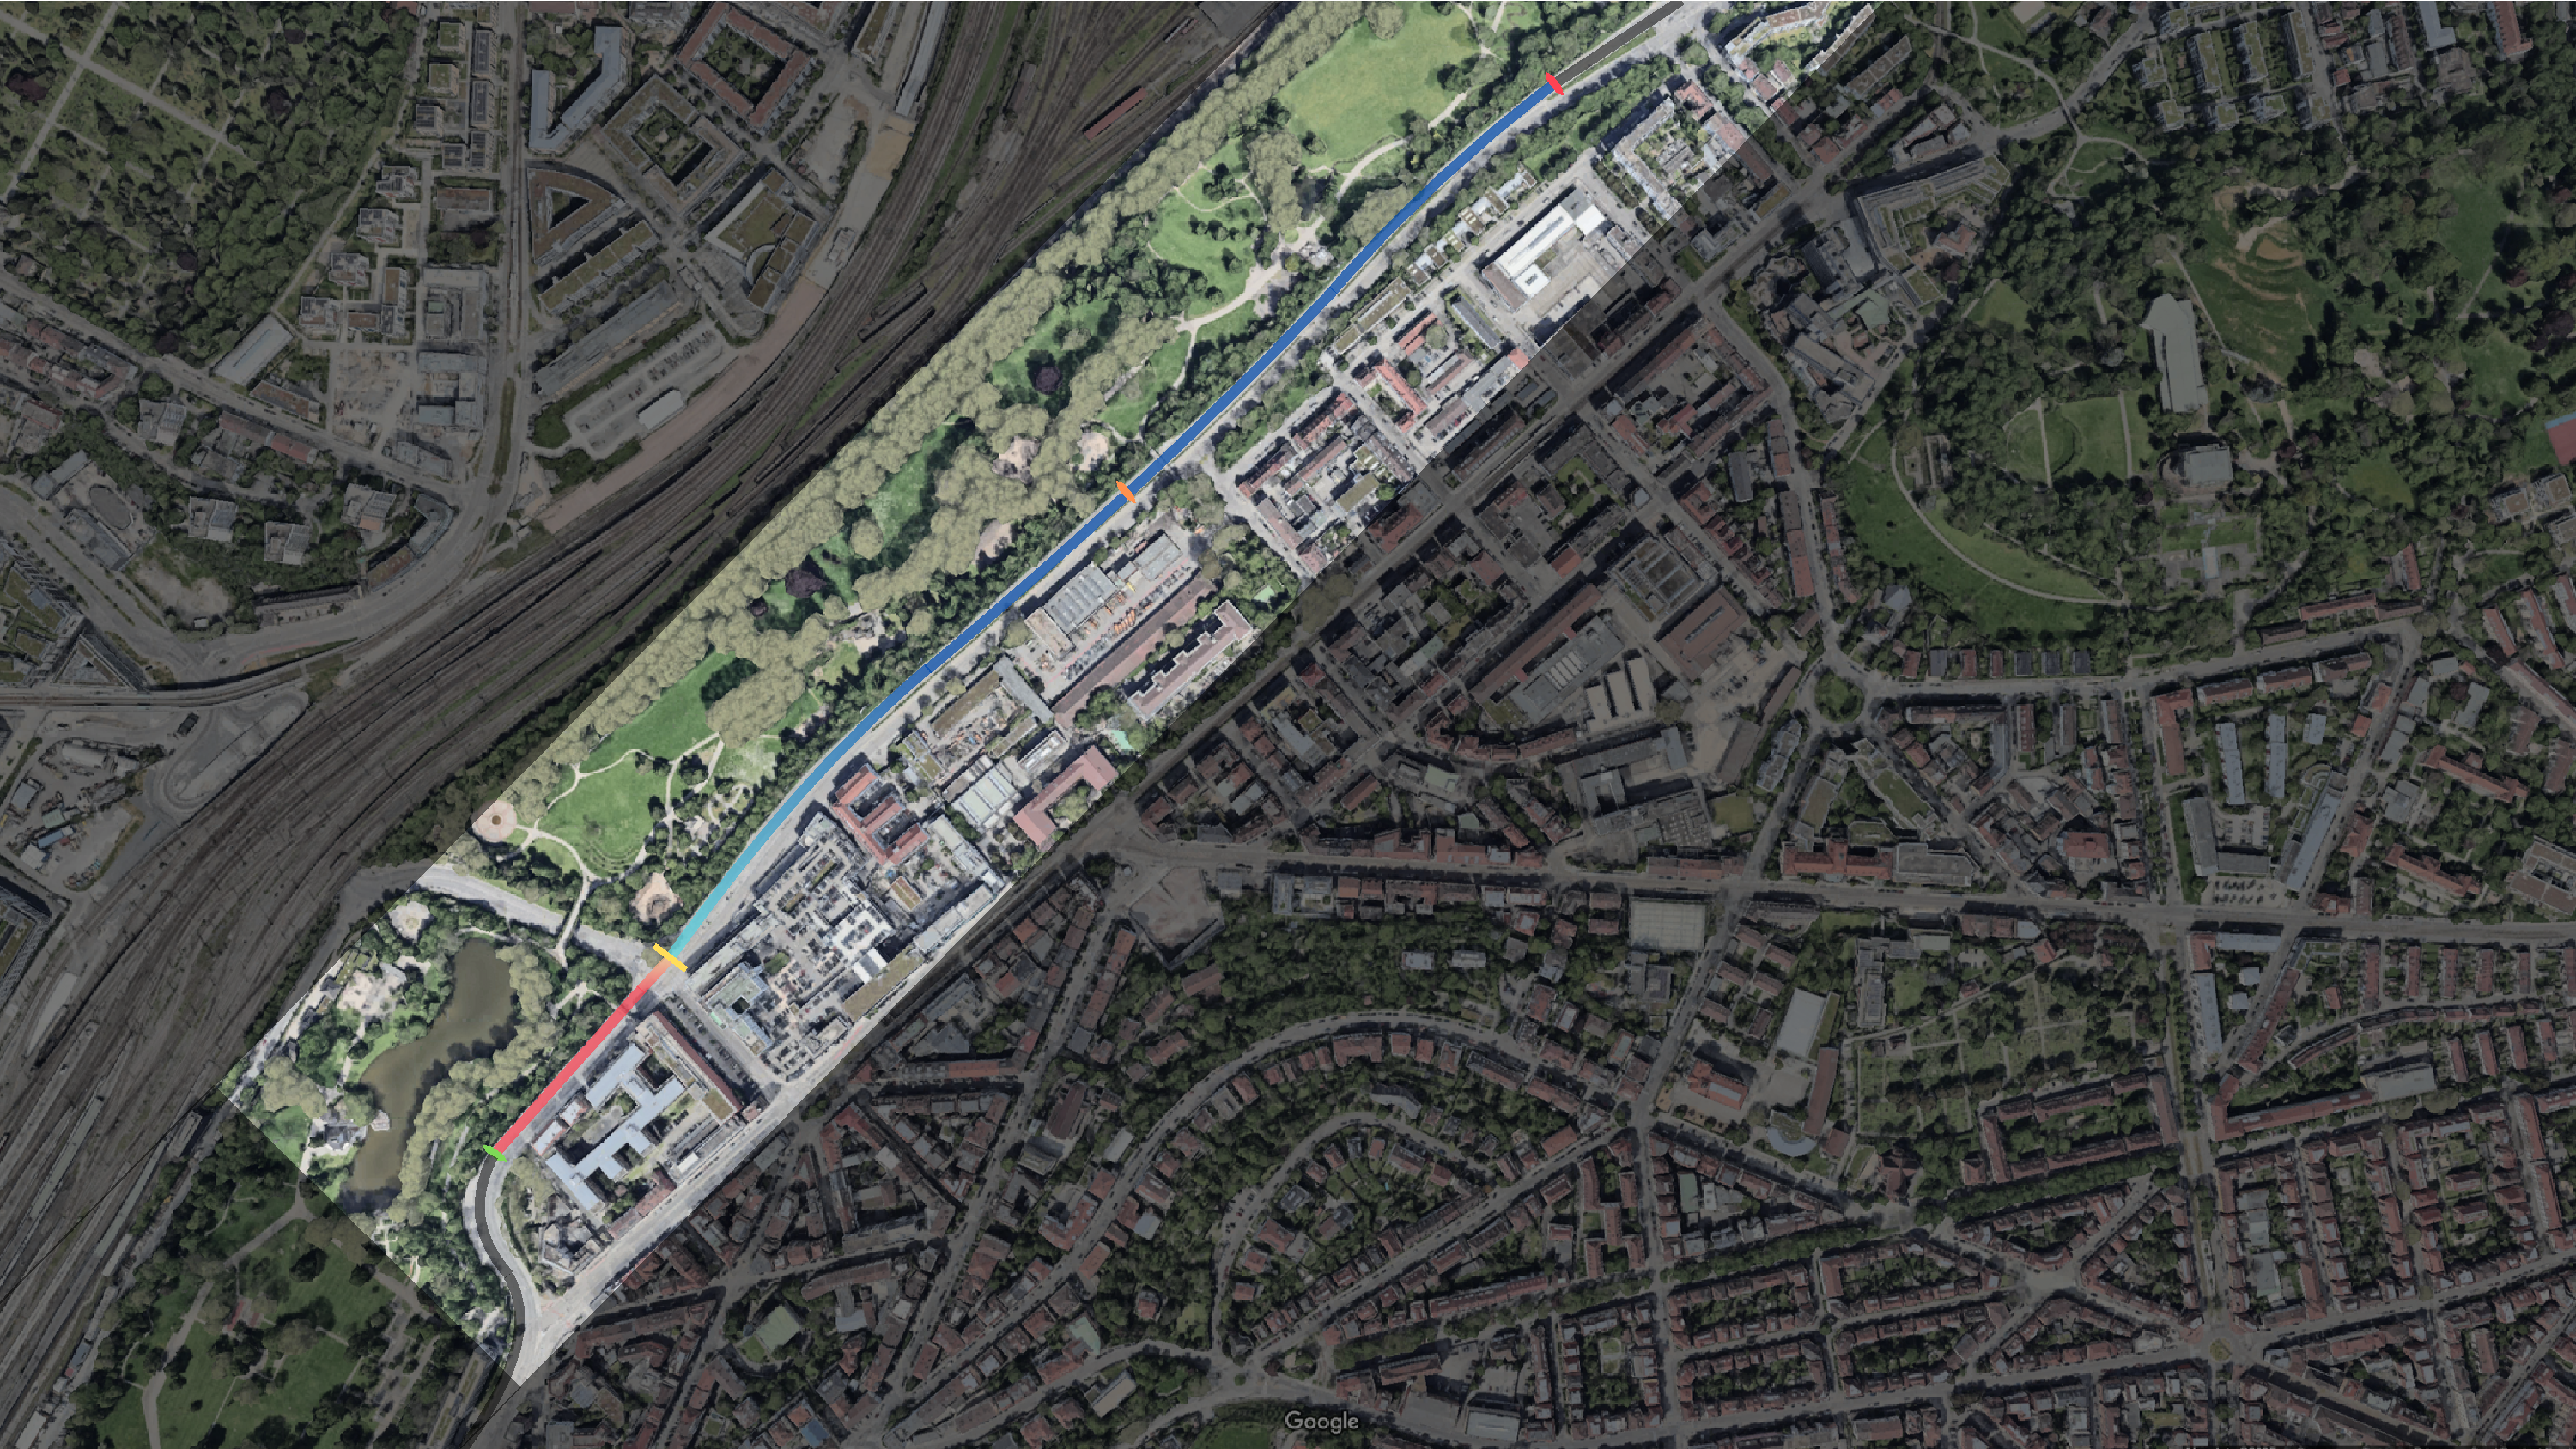
\includegraphics[width=\linewidth, page=1]{data/img/Neckartor/StuttgartNeckartorReal.pdf}
    \caption[Neckartor junction satellite image]{Satellite imagery of the real-world Neckartor junction in Stuttgart, highlighting the complex geometry and surrounding urban environment.}
    \label{fig:NeckartorMapReal}
  \end{subfigure}
  \hfill
  \begin{subfigure}[b]{0.49\textwidth}
    \includegraphics[width=\linewidth, page=1]{data/img/Neckartor/StuttgartNeckartorSumo.pdf}
    \caption[Digital twin of Neckartor in \ac{sumo}]{The digital twin of the Neckartor junction as implemented in the \ac{sumo} environment, showing the modelled lanes and connections.}
    \label{fig:NeckartorMapSUMO}
  \end{subfigure}
  \caption[Real-World vs. Simulated Neckartor Junction]{%
  Comparison of the real-world Neckartor junction (left) with its high-fidelity digital twin in the \ac{sumo} simulation (right). 
  The red segment marks the downstream cordon, while the blue segment indicates the upstream cordon. 
  The yellow line represents the signalized intersection. 
  Red square dots denote the start points for the $1000\unit{\metre}$ downstream advisory range, while orange square dots denote the start points for the $500\unit{\metre}$ range. 
  The green square marks the corresponding upstream end point of each advisory range. 
  Yellow arrows indicate the driving direction in each lane.}
  \label{fig:NeckartorMapComparison}
\end{figure}

Traffic demand is generated synthetically but is anchored to real-world loop detector data from the B14 corridor. The generated flow levels span the full spectrum of traffic states, from light, uncongested conditions to heavy, oversaturated congestion. Within each scenario, vehicles are introduced into the network with uniform inter-arrival times. Route assignment follows an equal probability distribution across all legitimate movements to ensure a balanced saturation of all lane groups. The \ac{glosa} \ac{mpr} is treated as a primary experimental variable, systematically tested in $10\%$ increments from $0\%$ (no equipped vehicles) to $100\%$ (fully equipped fleet). To manage this, two statistically independent insertion streams are used, allowing \ac{glosa}-equipped and non-equipped vehicles to coexist and interact within the same network environment.
\mynewline
The longitudinal driving behaviour for all vehicles is governed by the \ac{eidm}, a model chosen for its demonstrated ability to realistically capture stop-and-go waves and queue discharge dynamics. To ensure the simulation reflects real-world driver diversity, a heterogeneous fleet is synthesized by defining a combination of eleven fixed and eleven variable vehicle parameters. The fixed parameters, which establish baseline physical and behavioural constraints for all vehicles, are detailed in Table~\vref{tab:FixedFleetParams}. The variable parameters, listed in Table~\vref{tab:VariableFleetParams}, are sampled independently of uniform distributions over their specified ranges for each vehicle at spawn time. This methodology produces a rich vehicle population with a plausible span of physical dimensions (e.g., length and width) and driver characteristics (e.g., aggressiveness, reaction time), preventing a bias towards any single calibration point.
\mynewline

\begin{table}[htb]
  \centering
  \caption[Variable Vehicle Fleet Parameters]{Variable vehicle parameters used to synthesize the heterogeneous fleet in \ac{sumo}. Each parameter is drawn independently of a uniform distribution over the specified range at vehicle spawn time to ensure a realistic mix of driver behaviours and vehicle types. Derived from Lenz \cite{Lenz2024}.}
  \label{tab:VariableFleetParams}
  \resizebox{\textwidth}{!}{%
    \begin{tabular}{l l c c}
      \toprule
      \textbf{Parameter} & \textbf{Explanation} & \textbf{Min Value} & \textbf{Max Value} \\
      \midrule
      minGap & Minimum vehicle gap at standstill & $0.5\unit{m}$ & $4\unit{m}$ \\
      accel & Maximum acceleration & $0.97\unit{m\,s^{-2}}$ & $4\unit{m\,s^{-2}}$ \\
      startupDelay & Time delay until vehicle starts moving & $0.0\unit{s}$ & $2.0\unit{s}$ \\
      tau & Time headway maintained to the preceding vehicle & $0.5\unit{s}$ & $1.5\unit{s}$ \\
      delta & Influences how the vehicle reacts to speed differences & $1.0$ & $4.97$ \\
      treaction & Driver's reaction time & $0.2\unit{s}$ & $0.9\unit{s}$ \\
      tacmax & Time the vehicle needs to reach maximum acceleration & $0.5\unit{s}$ & $3.0\unit{s}$ \\
      Mflatness & \enquote{Flatness} of the acceleration and deceleration behavior & $1.0$ & $5.0$ \\
      Mbegin & Parameter for starting behavior & $0.1$ & $1.49$ \\
      length & Length of the vehicle & $2.2\unit{m}$ & $9.3\unit{m}$ \\
      width & Width of the vehicle & $1.5\unit{m}$ & $2.5\unit{m}$ \\
      \bottomrule
    \end{tabular}%
  }
\end{table}

\begin{table}[htb]
  \centering
  \caption[Fixed Vehicle Fleet Parameters]{Fixed vehicle parameters shared by all vehicles in the simulation fleet. These values define baseline behaviours and physical constraints, ensuring consistent dynamics across the entire population. Derived from Lenz \cite{Lenz2024}.}
  \label{tab:FixedFleetParams}
  \resizebox{\textwidth}{!}{%
    \begin{tabular}{l l c}
      \toprule
      \textbf{Parameter} & \textbf{Explanation} & \textbf{Value} \\
      \midrule
      decel & Maximum deceleration & $2.5\unit{m\,s^{-2}}$ \\
      emergencyDecel & Maximum emergency braking deceleration & $15\unit{m\,s^{-2}}$ \\
      tpreview & Time horizon a vehicle "looks" into the future to plan speed & $4\unit{s}$ \\
      tPersDrive & Duration the vehicle remains in continuous driving mode & $3\unit{s}$ \\
      tPersEstimate & Duration the vehicle remains in estimation mode & $10\unit{s}$ \\
      coolness & Influences how calmly or aggressively a vehicle reacts to disturbances & $0.99$ \\
      signaleader & Inaccuracy of speed adaptation to the preceding vehicle & $0.02$ \\
      sigmaerror & Inaccuracy regarding errors in driving style (speed, distance) & $0.1$ \\
      sigmagap & Inaccuracy of the gap to the preceding vehicle & $0.1$ \\
      jerkmax & Maximum rate of change of acceleration & $3\unit{m\,s^{-3}}$ \\
      epsilonacc & Inaccuracy of acceleration estimation & $1.0$ \\
      \bottomrule
    \end{tabular}%
  }
\end{table}

Each simulation is run for a total temporal horizon of $43.33\unit{min}$. The initial $10\unit{min}$ of this period serves as a warm-up phase, which allows traffic flows to stabilize and ensures that initial transient effects do not influence the results. Consequently, only data from the final $33.33\,\unit{min}$ are used for statistical analysis. A simulation time step of $0.1\unit{s}$ is maintained to provide sufficient resolution for both the \ac{eidm}'s dynamic equations and for the accurate integration of instantaneous emissions. For data collection, the analysis is spatially constrained to a corridor extending $1\unit{km}$ upstream and $200\,\unit{m}$ downstream from the intersection's primary stop line. This spatial clipping focuses the evaluation on the region most directly influenced by the \ac{glosa} advisories.
\mynewline
For each simulated vehicle, a dedicated log file is generated that records a high-resolution time series of its state, including timestamp, position, speed, and acceleration. Instantaneous emission rates for all relevant pollutants are concurrently calculated using \ac{sumo}’s internal emission model back-ends. To facilitate post-processing with external analysis scripts, these logs are flushed at every simulation step. A consistent configuration is applied across all scenarios to ensure the comparability of results throughout the comprehensive sweeps of traffic flow, market penetration, and other experimental parameters.



\section{Execution Protocol and Parameterization}
\label{sec:exec_protocol}

The execution protocol translates the conceptual design into a reproducible set of simulation runs that sample all relevant boundary conditions while keeping computational cost within practical limits. Reproducibility is guaranteed by fixing the random seed to \texttt{12345}; thus every pseudo-random operation like route choice, lane assignment, and vehicle parameter draw, yields identical sequences across repeated executions. Each run evaluates one of two \ac{glosa} algorithm variants: (i) the \emph{baseline} or \emph{flow-optimised} controller, which targets minimum delay, and (ii) the \emph{eco-driving} controller, which minimises fuel use but ignores explicit queue effects. For every algorithm, the parameter sweep enumerates all combinations of traffic flow, market penetration, and communication range, leading to $176$ distinct scenarios per controller and hence $352$ in total. An overview of all the parameters is given in Table \ref{tab:ScenarioMatrix}. The three independent factors are detailed below.  

\begin{enumerate}
\item \textbf{Traffic flow.} Eight demand levels are enforced by limiting the number of inserted vehicles to 50, 100, 250, 500, 1000, 1500, 2000, and 2500, corresponding to 69, 138, 346, 692, 1385, 2077, 2769, and 3462\,veh\,h\(^{-1}\), respectively.  
\item \textbf{Market penetration.} The \ac{glosa} \ac{mpr} varies from 0\,\% to 100\,\% in 10-percentage-point increments. A Bernoulli draw at spawn time classifies each vehicle as equipped or non-equipped, producing two statistically independent traffic streams within the same macroscopic flow.
\item \textbf{Communication range.} Prior work by Lenz \cite{Lenz2024} found no statistically significant difference between 500\,m and 1000\,m communication horizons; therefore only the 500\,m radius is tested here but retained as a formal factor to keep the full Cartesian design consistent with earlier literature. The advisory is sent whenever an equipped vehicle’s distance to the stop line is $\gls{dup}\leq500\,\mathrm{m}$ and $\gls{ddown}\leq200\,\mathrm{m}$.
\end{enumerate}

All other settings are held constant across the sweep. The optimiser assumes an additional fixed switch time of 2.1\,s to capture actuation delays between the traffic controller and the actual signal head. Slack time \(\gls{tslack}\) is sampled uniformly in the closed interval \([0.1,5]\,\mathrm{s}\) at run time, reflecting uncertainty in residual phase duration. Downstream distance is clipped to 200\,m, matching the evaluation window specified in Section~\ref{sec:SimEnvironment}. A yellow-phase buffer of \(0.5\,\mathrm{s}\) prevents infeasible trajectories that might straddle the amber interval. The numerical search increment for the longitudinal optimiser, \(\Delta a\), is fixed to \(0.01\,\mathrm{m\,s^{-2}}\); preliminary tests confirmed that smaller steps add negligible accuracy but inflate computation time. Objective-function weights follow \(\alpha_{\text{speed}}=1.0\) and \(\alpha_{\text{reach}}=0.5\). Speed estimation downstream uses one-second velocity samples, which balances responsiveness with noise suppression.
\mynewline
Emissions and energy demand are assessed with two fuel models, \ac{hbefa} 4 and \textsc{PHEMlight} 5, specified in section \ref{subsubsec:detailed_emission_models}. Queue length is forcibly set to zero in all optimiser calls, thereby isolating pure speed-advice effects from more complex queue-estimation feedback loops.

\begin{table}[tbp]
  \centering
  \caption{Scenario design matrix per algorithm.  Each cell is executed once with seed~\texttt{12345}.}
  \label{tab:ScenarioMatrix}
  \begin{tabular}{ccccc}
    \toprule
    Factor & Symbol & Levels & Values & Unit \\
    \midrule
    Traffic flow & \(Q\) & 8 & 69–3462 & veh\,h\(^{-1}\) \\
    Market penetration & MPR & 11 & 0–100 (step 10) & \% \\
    Comm.\ range & \(r_{\text{com}}\) & 2 & 500, 1000 & m \\
    \midrule
    \multicolumn{2}{c}{Total scenarios} & \multicolumn{3}{c}{\(8\times11\times2=176\)}\\
    \bottomrule
  \end{tabular}
\end{table}

The optimizer assesses potential speed profiles within the specified communication range of 500 meters prior to and 200 meters following the intersection during runtime. Upstream motion is constrained by the extended \ac{eidm} envelope described in Section~\ref{sec:SimEnvironment}. The controller solves a univariate line search over acceleration \(a_{\text{up}}\) with step \(\Delta a\). Terminal conditions are checked at the downstream horizon \(l=200\,\mathrm{m}\); trajectories violating \(\gls{vmin}\) or \(\gls{bmax}\) are discarded. 
\mynewline
The resulting dataset underpins all metrics specified in Section~\ref{sec:performance_evaluation}. Because the protocol controls every stochastic degree of freedom and stores exhaustive logs, future researchers can reproduce the study by re-running the same configuration files and seed. Any deviation, such as a different communication horizon or an additional queue-aware variant, would simply append new factors to the Cartesian design while preserving the core template documented here.


\section{Performance Metrics and Evaluation Methodology}
\label{sec:performance_evaluation}

The assessment framework is designed to expose the trade-off between smoother traffic flow and ecological benefit introduced by the two \ac{glosa} variants. All quantities are derived from the trajectory and emission logs produced by \ac{sumo}. Each scenario is executed exactly once with a fixed random seed, yielding a single deterministic outcome; therefore, statistical confidence intervals are not applicable.

\paragraph{Microscopic Traffic Efficiency.}
The quality of longitudinal driving behaviour is quantified using four primary indicators:

\begin{enumerate}[label=\textbf{(\roman*)}]
    \item \textbf{Stops per Vehicle:} The stop frequency, \gls{nstop}, is a key metric for traffic disruption. A stop is defined as an event where a vehicle's speed drops below a threshold of $2\unit{\metre\per\second}$ after having been above it. For a single vehicle $i$, the total number of stops is calculated as:
    \begin{equation}
        N_{\mathrm{stop},i} = \sum_{k=2}^{K}{\mathbbm{1}}(v_{i,k} < 2 \land v_{i,k-1} \ge 2)
    \end{equation}
    The scenario average, $\bar{N}_{\mathrm{stop}}$, is the mean of this value over all $N$ vehicles.

    \item \textbf{Mean Vehicle Speed:} The average speed, $\bar{v}$, serves as a measure of overall network mobility and is computed over all vehicles and all recorded time steps:
    \begin{equation}
        \bar{v} = \frac{1}{NK}\sum_{i=1}^{N}\sum_{k=1}^{K} v_{i,k}
    \end{equation}

    \item \textbf{Mean Absolute Acceleration:} As a surrogate for passenger comfort and powertrain strain, the mean absolute acceleration is calculated as:
    \begin{equation}
        \overline{|a|} = \frac{1}{NK}\sum_{i=1}^{N}\sum_{k=1}^{K} |a_{i,k}|
    \end{equation}

    \item \textbf{Mean Absolute Jerk:} To quantify the smoothness of acceleration changes, the mean absolute jerk, \gls{j}, is computed. Lower values indicate smoother, more comfortable driving profiles.
    \begin{equation}
        \overline{|j|} = \frac{1}{NK}\sum_{i=1}^{N}\sum_{k=1}^{K} |j_{i,k}|
    \end{equation}
\end{enumerate}

\paragraph{Macroscopic Throughput.}
Throughput is quantified by the mean number of vehicles crossing the intersection's stop-line detector per signal cycle. For a cycle length of $T_{\mathrm{cycle}}=120\unit{\second}$ with two green intervals, $I_{1}=[2,35]\unit{\second}$ and $I_{2}=[62,96]\unit{\second}$, the number of vehicles $N_{c}$ detected during cycle $c$ is:
\begin{equation}
    N_{c} = \#\lbrace i : t_{i,\mathrm{detection}} \in I_{1} \cup I_{2} \rbrace
\end{equation}
where $t_{i,\mathrm{detection}}$ is the time vehicle $i$ is detected at the stop line. The average per-cycle throughput is then $\overline{N}_{\mathrm{cycle}} = \frac{1}{C}\sum_{c=1}^{C} N_{c}$.

\paragraph{Energy Demand and Pollutant Emissions.}
The environmental impact is characterised by per-vehicle pollutant rates, with \ac{co2} as the primary metric for fuel consumption. Emissions are computed over the $1.2\unit{\kilo\metre}$ evaluation corridor by summing the instantaneous rates in the log, multiplying by the time step $\Delta t = 0.1\unit{\second}$, and normalising by distance:
\begin{equation}
    e_{i} = \frac{1}{1000 \cdot L} \sum_{k=s_i}^{e_i} \dot{m}^{\mathrm{CO_2}}_{k} \cdot \Delta t, \quad \text{where } L = 1.2\,\mathrm{km}
\end{equation}
The same form applies to \ac{nox} emissions. The analysis is performed in parallel for both the HBEFA4 and PHEMlight5 emission models.

\paragraph{Relative Performance and Break-Even Analysis.}
To facilitate comparisons, each metric $y$ is expressed as a percentage deviation from the uncontrolled baseline (0\% \ac{mpr}). A break-even analysis is conducted by directly comparing the performance of the \ac{eco-glosa} and \ac{flow-glosa} controllers at each discrete combination of traffic flow and \ac{mpr}. This identifies which controller provides a superior outcome under specific conditions.

\paragraph{Computational Viability.}
The practical feasibility of each algorithm is assessed by recording and comparing the absolute wall-clock time required to complete each simulation scenario. The incremental cost of the eco-driving algorithm is evaluated by comparing its runtime, $T_{\mathrm{traci,eco}}$, against that of the less complex flow-optimised baseline, $T_{\mathrm{traci,flow}}$.

\paragraph{Visualisation Strategy.}
The results are conveyed using a harmonised set of graphical summaries:
\begin{enumerate}[label=\textbf{(\alph*)},leftmargin=*]
    \item \textbf{Line Charts:} Key metrics such as mean speed, stop frequency, and \ac{co2} emissions are plotted as functions of \ac{mpr}. Each traffic demand level is shown in a separate panel to facilitate direct comparison across different levels of congestion.
    \item \textbf{Heat Maps:} The relative performance difference in \ac{co2} emissions between the two controllers is displayed on a two-dimensional grid of traffic flow versus penetration rate. This provides a clear overview of the operating regimes where each strategy delivers a net environmental benefit.
    \item \textbf{Break-Even Boundary:} On the 2D heat maps, the break-even penetration rate, $p^{\star}$, is traced as a boundary line. The line is solid black where the performance crossover is clear and decisive, and a dashed gray line where the transition is ambiguous or the performance difference is negligible.
\end{enumerate}
As each data point is derived from a single deterministic simulation run, no statistical error bars are presented.

\paragraph{Interpretation Focus.}
The subsequent analysis of results concentrates on two primary objectives: (i) to quantify the absolute and relative reductions in \ac{co2} emissions achieved by the eco-driving algorithm, and (ii) to identify the specific penetration-demand corridors where these ecological benefits can be achieved without significantly degrading traffic throughput. By normalizing all performance metrics against a baseline and indexing them by market penetration, this evaluation methodology yields transparent and scalable insights, ensuring the findings provide a robust foundation for future work involving new algorithms or network geometries.
\mynewline
The remainder of this chapter is dedicated to a detailed discussion of these results, structured by the key performance indicators. Section~\vref{sec:Results_GreenPhaseFlow} begins by evaluating the intersection's macroscopic throughput. The analysis then moves to microscopic traffic efficiency, examining the average vehicle speed in Section~\vref{sec:Results_MeanSpeed} and the vehicle stop frequency in Section~\vref{sec:Results_Stops}. Driving smoothness is assessed in Section~\vref{sec:Results_Smoothness} by analysing both the mean absolute acceleration and mean absolute jerk. Subsequently, Section~\vref{sec:Results_Emissions} details the environmental impact, focusing on \ac{co2} and \ac{nox} emissions. The core trade-offs are synthesised in Section~\vref{sec:Results_BreakEven}, which presents the break-even analysis. Finally, the practical feasibility is evaluated in Section~\vref{sec:Results_Computational} by comparing the computational runtimes of the two algorithms.

    \cleardoublepage

    \chapter{Results and Discussion}
\label{ch:ResultsDiscussion}

The preceding chapters defined a rigorous simulation framework and parameter sweep for both flow-optimised and eco-driving \ac{glosa} controllers. We now explore how these algorithms perform under varying traffic loads and penetration rates, revealing their network-level and vehicle-level impacts.  
We open with an analysis of green‐phase vehicle flow to understand discharge performance under connected control (\ref{sec:Results_GreenPhaseFlow}). From there, attention moves to vehicle dynamics: first average travel speed (\ref{sec:Results_MeanSpeed}), then stop frequency (\ref{sec:Results_Stops}), and finally driving smoothness via acceleration profiles (\ref{sec:Results_Smoothness}). Environmental consequences follow, as per-vehicle CO$_2$ and NO$_x$ emissions, quantify ecological benefit (\ref{sec:Results_Emissions}). A dedicated break-even analysis then pinpoints the critical penetration at which eco-driving gains outweigh flow-optimised advantages (\ref{sec:Results_BreakEven}). Computational viability comes next, comparing runtime overheads of the advisory loop and optimisation algorithm (\ref{sec:Results_Computational}). We conclude by synthesising these findings, discussing trade-offs and implications for real-world deployment (\ref{sec:Results_Discussion}).  

\section{Green‐Phase Vehicle Flow}
\label{sec:Results_GreenPhaseFlow}

The per-cycle vehicle flow for demand levels ranging from $69$ to $3462~\unit{\veh\per\hour}$ across \acp{mpr} is summarized in Table~\vref{tab:GreenPhaseFlow}. \enquote{Standard} ($0\%$) denotes no \ac{glosa}, and \enquote{Baseline} denotes \ac{flow-glosa}. Figure~\vref{fig:combined_flow} visualise the curves for HBEFA4 and PHEMlight5 at $2077$, $2769$ and $3462~\unit{\veh\per\hour}$. At low to moderate demand ($69$--$692~\unit{\veh\per\hour}$), both \ac{eco-glosa} and \ac{flow-glosa} remain within $\pm0.04\unit{\veh\per\hour}$ of the Standard across the full \ac{mpr} range. This implies that speed advisories, regardless of whether they are emission- or flow-optimized, do not significantly impact green-phase capacity in the presence of low traffic densities. Beyond the $2077~\unit{\veh\per\hour}$ breakpoint, the throughput of the \ac{eco-glosa} controller declines sharply. For instance, at a demand of $2769~\unit{\veh\per\hour}$ under the PHEMlight5 model, the flow drops from $46.03$ vehicles at Standard to $35.90$ vehicles at $90\%$ \ac{mpr}, a reduction of $22\%$. A similar decline occurs at $3462~\unit{\veh\per\hour}$ with the HBEFA4 model, where throughput falls from $49.03$ to $37.27$ vehicles at full \ac{mpr}. This provides clear evidence of queue formation and spill‐back occurring within a single green phase. In contrast, the \ac{flow-glosa} baseline curves exhibit modest throughput gains at high penetration under heavy demand, increasing flow above the Standard by up to $17.5\%$ at $3462~\unit{\veh\per\hour}$. The findings of this study confirm, that \ac{eco-glosa} does not affect the flow at low densities, but its emission-driven advisories incur substantial capacity penalties during periods of high demand. Conversely, \ac{flow-glosa} not only maintains, but also improves green-phase capacity at full penetration.

\begin{figure}[htbp]
  \centering
  % first two subfigures
  \begin{subfigure}[t]{0.98\textwidth}
    \includegraphics[width=\textwidth]{data/img/GreenPhaseVehicleFlow/GreenPhaseVehicleFlow_Cars1500.pdf}
    \caption{$2077~\unit{\veh\per\hour}$}
    \label{fig:flow_2077}
  \end{subfigure}\hfill
  \begin{subfigure}[t]{0.98\textwidth}
    \includegraphics[width=\textwidth]{data/img/GreenPhaseVehicleFlow/GreenPhaseVehicleFlow_Cars2000.pdf}
    \caption{$2769~\unit{\veh\per\hour}$}
    \label{fig:flow_2769}
  \end{subfigure}
  \caption[Green–phase vehicle flow vs. \ac{mpr} at $2077$ and $2769~\unit{\veh\per\hour}$]{%
    Green–phase vehicle flow as a function of \ac{mpr} for two high‐demand scenarios. Each plot compares the Standard (no \ac{glosa}), \ac{eco-glosa} (HBEFA4 and PHEMlight5), and \ac{flow-glosa} controllers at $2077$ and $2769~\unit{\veh\per\hour}$.%
  }
  \label{fig:combined_flow}
\end{figure}

\begin{figure}[htbp]\ContinuedFloat
  \centering
  % remaining subfigure on next page
  \begin{subfigure}[t]{0.98\textwidth}
    \includegraphics[width=\textwidth]{data/img/GreenPhaseVehicleFlow/GreenPhaseVehicleFlow_Cars2500.pdf}
    \caption{$3462~\unit{\veh\per\hour}$}
    \label{fig:flow_3462}
  \end{subfigure}
  \caption[]{%
    (continued) Green–phase vehicle flow as a function of \ac{mpr} for the high‐demand scenario at $3462~\unit{\veh\per\hour}$.%
  }
\end{figure}

The primary cause for this behaviour is an inherent design constraint of the \ac{eco-glosa} algorithm: it only provides speed advisories that are equal to or less than the vehicle's initial speed. At high traffic densities ($2769~\unit{\veh\per\hour}$ and above), this conservative approach systematically reduces the average speed of equipped vehicles. As the penetration rate increases, the overall platoon velocity decreases, leading to platoon compression. Consequently, the number of vehicles arriving at the intersection exceeds the capacity that can be discharged during the green phase, resulting in queue formation and the onset of congestion. In these dense traffic conditions, unequipped vehicles have limited ability to manoeuvre or bypass the slower-moving equipped vehicles, forcing them to adopt the reduced platoon speed and further contributing to the decline in throughput. This progressive speed reduction is confirmed by the average vehicle speed data presented in the following section.
\mynewline
This phenomenon is changed under the PHEMlight5 emission model. PHEMlight5 assigns a higher cost penalty to even minor acceleration events. To minimise these costs, the \ac{eco-glosa} controller advises even more conservative speed profiles, which accelerates the onset of congestion at lower demand levels, as observed at $2769~\unit{\veh\per\hour}$.
Furthermore, this mechanism explains the severe, non-recoverable congestion indicated by outliers in the results of HBEFA4 at a demand of $2769~\unit{\veh\per\hour}$. When a vehicle, already slowed by incipient congestion, receives a new advisory, \ac{eco-glosa} is unable to recommend a higher speed even if conditions ahead improve. This vehicle becomes a persistent moving bottleneck, initiating a cascading failure by forcing subsequent vehicles to reduce their speed. This domino effect progressively degrades the overall traffic flow as newly arriving \ac{eco-glosa} vehicles receive increasingly lower speed advisories.
\mynewline
In contrast, the \ac{flow-glosa} controller is designed to maximise throughput and is permitted to advise acceleration. This allows it to issue higher speed advisories to slower vehicles, enabling them to catch up to the green wave and increase the vehicle discharge rate per cycle. This fundamental design difference explains why \ac{flow-glosa} can improve capacity where \ac{eco-glosa}, by design, can only maintain or reduce it.

\begin{table}[htb]
  \centering
  \caption[Green-phase vehicle throughput for all volumes and \ac{mpr} values]{Green-phase vehicle throughput, measured in vehicles per cycle, across all simulated traffic volumes and \ac{mpr} values. The Standard scenario denotes uncontrolled traffic ($0\%$ \ac{mpr}), while Baseline refers to the \ac{flow-glosa} controller.}
  \label{tab:GreenPhaseFlow}
  \resizebox{\textwidth}{!}{%
  \begin{tabular}{r l l r *{10}{r}}
    \toprule
    Vehicles & Algorithm                   & Fuel Model       & \textbf{0\% (Standard)} & 10\%  & 20\%  & 30\%  & 40\%  & 50\%  & 60\%  & 70\%  & 80\%  & 90\%  & 100\% \\
    \midrule
    69   & \ac{eco-glosa}              & HBEFA4           & \textbf{1.17} & 1.17  & 1.17  & 1.17  & 1.17  & 1.13  & 1.17  & 1.17  & 1.13  & 1.17  & 1.17  \\
    69   & Baseline (\ac{flow-glosa})  & HBEFA4           & \textbf{1.17} & 1.17  & 1.17  & 1.17  & 1.17  & 1.13  & 1.17  & 1.17  & 1.17  & 1.17  & 1.17  \\
    69   & \ac{eco-glosa}              & PHEMLIGHT5       & \textbf{1.17} & 1.17  & 1.17  & 1.17  & 1.17  & 1.13  & 1.17  & 1.17  & 1.17  & 1.17  & 1.17  \\
    69   & Baseline (\ac{flow-glosa})  & PHEMLIGHT5       & \textbf{1.17} & 1.17  & 1.17  & 1.17  & 1.17  & 1.13  & 1.17  & 1.17  & 1.17  & 1.17  & 1.17  \\
    \midrule
    138  & \ac{eco-glosa}              & HBEFA4           & \textbf{2.30} & 2.30  & 2.30  & 2.27  & 2.27  & 2.27  & 2.27  & 2.30  & 2.30  & 2.27  & 2.27  \\
    138  & Baseline (\ac{flow-glosa})  & HBEFA4           & \textbf{2.30} & 2.30  & 2.30  & 2.30  & 2.27  & 2.27  & 2.27  & 2.30  & 2.30  & 2.30  & 2.27  \\
    138  & \ac{eco-glosa}              & PHEMLIGHT5       & \textbf{2.30} & 2.30  & 2.30  & 2.27  & 2.27  & 2.27  & 2.27  & 2.30  & 2.30  & 2.30  & 2.27  \\
    138  & Baseline (\ac{flow-glosa})  & PHEMLIGHT5       & \textbf{2.30} & 2.30  & 2.30  & 2.30  & 2.27  & 2.27  & 2.27  & 2.30  & 2.30  & 2.30  & 2.27  \\
    \midrule
    346  & \ac{eco-glosa}              & HBEFA4           & \textbf{5.73} & 5.70  & 5.77  & 5.73  & 5.73  & 5.77  & 5.73  & 5.73  & 5.73  & 5.70  & 5.73  \\
    346  & Baseline (\ac{flow-glosa})  & HBEFA4           & \textbf{5.73} & 5.73  & 5.77  & 5.70  & 5.73  & 5.73  & 5.77  & 5.70  & 5.73  & 5.70  & 5.73  \\
    346  & \ac{eco-glosa}              & PHEMLIGHT5       & \textbf{5.73} & 5.73  & 5.73  & 5.70  & 5.77  & 5.73  & 5.73  & 5.70  & 5.70  & 5.70  & 5.77  \\
    346  & Baseline (\ac{flow-glosa})  & PHEMLIGHT5       & \textbf{5.73} & 5.73  & 5.77  & 5.70  & 5.73  & 5.73  & 5.77  & 5.70  & 5.73  & 5.70  & 5.73  \\
    \midrule
    692  & \ac{eco-glosa}              & HBEFA4           & \textbf{11.57} & 11.60 & 11.57 & 11.57 & 11.60 & 11.57 & 11.57 & 11.57 & 11.57 & 11.53 & 11.63 \\
    692  & Baseline (\ac{flow-glosa})  & HBEFA4           & \textbf{11.57} & 11.60 & 11.60 & 11.60 & 11.60 & 11.60 & 11.60 & 11.60 & 11.60 & 11.60 & 11.57 \\
    692  & \ac{eco-glosa}              & PHEMLIGHT5       & \textbf{11.57} & 11.57 & 11.53 & 11.53 & 11.57 & 11.57 & 11.60 & 11.57 & 11.50 & 11.53 & 11.63 \\
    692  & Baseline (\ac{flow-glosa})  & PHEMLIGHT5       & \textbf{11.57} & 11.60 & 11.60 & 11.60 & 11.60 & 11.60 & 11.60 & 11.60 & 11.60 & 11.60 & 11.57 \\
    \midrule
    1385 & \ac{eco-glosa}              & HBEFA4           & \textbf{23.03} & 22.97 & 23.07 & 22.97 & 23.03 & 23.10 & 23.03 & 23.03 & 22.97 & 23.07 & 23.03 \\
    1385 & Baseline (\ac{flow-glosa})  & HBEFA4           & \textbf{23.03} & 23.07 & 23.03 & 23.07 & 23.10 & 23.17 & 23.03 & 23.10 & 23.13 & 23.07 & 23.07 \\
    1385 & \ac{eco-glosa}              & PHEMLIGHT5       & \textbf{23.03} & 23.07 & 23.03 & 23.03 & 23.10 & 23.07 & 23.07 & 22.93 & 22.93 & 23.00 & 23.03 \\
    1385 & Baseline (\ac{flow-glosa})  & PHEMLIGHT5       & \textbf{23.03} & 23.07 & 23.03 & 23.03 & 23.10 & 23.07 & 23.07 & 22.93 & 22.93 & 23.00 & 23.03 \\
    \midrule
    2077 & \ac{eco-glosa}              & HBEFA4           & \textbf{34.63} & 34.70 & 34.67 & 34.63 & 34.67 & 34.63 & 34.70 & 34.63 & 34.63 & 34.63 & 34.67 \\
    2077 & Baseline (\ac{flow-glosa})  & HBEFA4           & \textbf{34.63} & 34.60 & 34.63 & 34.63 & 34.67 & 34.53 & 34.60 & 34.60 & 34.70 & 34.63 & 34.70 \\
    2077 & \ac{eco-glosa}              & PHEMLIGHT5       & \textbf{34.63} & 34.70 & 34.60 & 34.63 & 34.73 & 34.63 & 34.77 & 34.67 & 34.67 & 34.63 & 34.70 \\
    2077 & Baseline (\ac{flow-glosa})  & PHEMLIGHT5       & \textbf{34.63} & 34.60 & 34.63 & 34.63 & 34.67 & 34.53 & 34.60 & 34.60 & 34.70 & 34.63 & 34.70 \\
    \midrule
    2769 & \ac{eco-glosa}              & HBEFA4           & \textbf{46.03} & 46.10 & 46.03 & 41.90 & 42.67 & 46.20 & 39.30 & 46.30 & 46.07 & 46.03 & 46.03 \\
    2769 & Baseline (\ac{flow-glosa})  & HBEFA4           & \textbf{46.03} & 46.13 & 46.03 & 45.97 & 46.07 & 46.03 & 46.17 & 46.17 & 46.07 & 46.07 & 46.13 \\
    \textbf{2769} & \textbf{\ac{eco-glosa}} & \textbf{PHEMLIGHT5} & \textbf{46.03} & \textbf{44.47} & \textbf{41.73} & \textbf{39.33} & \textbf{38.37} & \textbf{37.57} & \textbf{37.17} & \textbf{36.97} & \textbf{36.67} & \textbf{35.90} & \textbf{37.83} \\
    2769 & Baseline (\ac{flow-glosa})  & PHEMLIGHT5       & \textbf{46.03} & 46.13 & 46.03 & 45.97 & 46.07 & 46.03 & 46.17 & 46.17 & 46.07 & 46.07 & 46.13 \\
    \midrule
    3462 & \ac{eco-glosa}              & HBEFA4           & \textbf{49.03} & 46.03 & 44.47 & 42.80 & 42.27 & 41.27 & 39.33 & 39.17 & 38.13 & 38.00 & 37.27 \\
    3462 & Baseline (\ac{flow-glosa})  & HBEFA4           & \textbf{49.03} & 49.67 & 48.97 & 48.97 & 49.17 & 49.13 & 53.53 & 49.17 & 57.53 & 57.57 & 57.60 \\
    3462 & \ac{eco-glosa}              & PHEMLIGHT5       & \textbf{49.03} & 44.07 & 41.33 & 39.50 & 38.77 & 37.53 & 37.03 & 36.67 & 36.47 & 36.33 & 36.17 \\
    3462 & Baseline (\ac{flow-glosa})  & PHEMLIGHT5       & \textbf{49.03} & 49.67 & 48.97 & 48.97 & 49.17 & 49.13 & 53.53 & 49.17 & 57.53 & 57.57 & 57.60 \\
    \bottomrule
  \end{tabular}%
  }
\end{table}


\section{Average Vehicle Speed}
\label{sec:Results_MeanSpeed}

Table~\ref{tab:MeanSpeed} and Figures~\ref{fig:MeanSpeed_2077}–\ref{fig:MeanSpeed_3462} report the mean cruise speed of the platoon as a function of \ac{mpr}. The three control strategies, Standard, \ac{eco-glosa} and \ac{flow-glosa}, are compared under both emission models (HBEFA4 and PHEMLIGHT5) at three critical demand levels. A careful examination of the data yields six principal insights.

\subparagraph*{1. Systematic impact of \ac{mpr} on \ac{eco-glosa}.}
Across \emph{all} volumes, \ac{eco-glosa} shows a monotonic speed decrease as \ac{mpr} increases. For example, at the lightest load of $69\,\mathrm{veh/h}$, the HBEFA4 mean speed drops from $13.34\,\mathrm{m/s}$ (Standard) to $13.01\,\mathrm{m/s}$ at $100\,\%$ \ac{mpr} ($\downarrow 2.5\,\%$). The reduction accelerates with demand: at $2077\,\mathrm{veh/h}$, the decrease is $0.44\,\mathrm{m/s}$ ($\downarrow 3.5\,\%$) by $40\,\%$ \ac{mpr}, while at $2769\,\mathrm{veh/h}$ it becomes catastrophic, falling from $11.94\,\mathrm{m/s}$ to $2.57\,\mathrm{m/s}$ ($\downarrow 79\,\%$) by $90\,\%$ \ac{mpr} under PHEMlight5 (Figure~\ref{fig:MeanSpeed_PHEM_2769}). This monotonic decline is, for example, illustrated in Figures~\ref{fig:MeanSpeed_HBEFA4_2077} and~\ref{fig:MeanSpeed_PHEM_2077}.

\subparagraph*{2. Flow stability and jam resolution of \ac{flow-glosa}.}
\ac{flow-glosa} maintains near-Standard speeds up to $2769\,\mathrm{veh/h}$, and under full saturation ($3462\,\mathrm{veh/h}$) it dissolves the queue once penetration exceeds approximately $80\%$. The mean speed increases from $\mathbf{3.86\,\mathrm{m/s}}$ (Standard, 0\% \ac{mpr}) to $4.16\,\mathrm{m/s}$ at $50\%$ \ac{mpr} and ultimately reaches $\mathbf{12.18\,\mathrm{m/s}}$ at $100\%$ \ac{mpr}. This behaviour demonstrates that \ac{flow-glosa} can actively resolve gridlock and restore free-flow speeds when a sufficient share of vehicles conforms to its advisory. The jam-dissolving capability is evident in Figures~\ref{fig:MeanSpeed_HBEFA4_3462} and~\ref{fig:MeanSpeed_PHEM_3462}.  


\subparagraph*{3. Emission-model sensitivity.}
PHEMlight5 consistently produces lower speeds than HBEFA4 at the same \ac{mpr} and demand level. The difference is modest at low demand (approximately $0.1\,\mathrm{m/s}$ for $69$--$346\,\mathrm{veh/h}$) but widens dramatically in congestion. At $2769\,\mathrm{veh/h}$ and $30\,\%$ \ac{mpr}, PHEMlight5--\ac{eco-glosa} already drops to $3.17\,\mathrm{m/s}$ versus $7.32\,\mathrm{m/s}$ for HBEFA4, a $57\,\%$ gap. This reflects the higher temporal resolution and the non-linear fuel--speed polynomial in PHEMlight5: it penalises short bursts of high engine power more strongly, which prompts earlier decelerations and thus longer queuing times. The widening gap between HBEFA4 and PHEMlight5 under congestion is visible in Figures~\ref{fig:MeanSpeed_HBEFA4_2769} and~\ref{fig:MeanSpeed_PHEM_2769}.

\subparagraph*{4. Jam-onset thresholds.}
Under the conventional jam criterion of around $v \leq 4\,\mathrm{m/s}$ in urban areas, Table~\ref{tab:MeanSpeed} reveals discrete breakpoints for the \ac{eco-glosa}. In the PHEMlight5 case, a jam forms at $10$--$20\,\%$ \ac{mpr} for $2769\,\mathrm{veh/h}$ and at the first non-zero \ac{mpr} for $3462\,\mathrm{veh/h}$. HBEFA4 postpones the jam onset by roughly one \ac{mpr} decade: $30$--$50\,\%$ at $2769\,\mathrm{veh/h}$. The staggered thresholds underscore the importance of the emission-model choice when extrapolating eco-driving benefits to congested corridors. The onset of jam (v\,$\le4\,\mathrm{m/s}$) corresponds to the inflection points in Figures~\ref{fig:MeanSpeed_HBEFA4_2769} and~\ref{fig:MeanSpeed_PHEM_2769}.

\subparagraph*{5. Residual overshoot at low demand.}
At sub-saturated volumes ($69$--$1385\,\mathrm{veh/h}$), \ac{eco-glosa} occasionally overshoots Standard by up to $0.04\,\mathrm{m/s}$ at $10\,\%$ \ac{mpr}. The effect, most visible in HBEFA4, originates from the algorithm's \enquote{anticipatory glide} that smooths minor stop-and-go waves, thereby shortening braking phases and slightly increasing the arithmetic mean of cruise speed. However, as soon as \ac{mpr} exceeds approximately $20\,\%$, the fuel-saving bias dominates and the curve bends downward. The slight overshoot at low demand (10\,\% \ac{mpr}) is observable in Figures~\ref{fig:MeanSpeed_HBEFA4_2077} and~\ref{fig:MeanSpeed_PHEM_2077}.

\subparagraph*{6. Progressive speed gains under \ac{flow-glosa}.}
As \ac{mpr} increases, \ac{flow-glosa} delivers measurable speed improvements even below saturation. At low demand ($69\,\mathrm{veh/h}$), HBEFA4–\ac{flow-glosa} speeds climb from $\mathbf{13.34}$ to $13.88\,\mathrm{m/s}$ ($+4.1\,\%$) by $90\,\%$ \ac{mpr}. At medium demand ($1385\,\mathrm{veh/h}$), the mean speed rises from $\mathbf{12.84}$ to $13.07\,\mathrm{m/s}$ ($+1.8\,\%$) at $100\,\%$ penetration. Even at high demand ($2769\,\mathrm{veh/h}$), it increases from $\mathbf{11.94}$ to $12.55\,\mathrm{m/s}$ ($+5.1\,\%$) at $100\,\%$ \ac{mpr}. These consistent gains underscore \ac{flow-glosa}’s capacity to smooth stop-and-go waves and improve throughput across light, moderate, and heavy traffic regimes. The progressive uplift with increasing penetration is shown by the upward slopes in Figures~\ref{fig:MeanSpeed_HBEFA4_2077}, \ref{fig:MeanSpeed_HBEFA4_2769}, and \ref{fig:MeanSpeed_HBEFA4_3462} (and similarly for PHEMLIGHT5 in Figures~\ref{fig:MeanSpeed_PHEM_2077}, \ref{fig:MeanSpeed_PHEM_2769}, \ref{fig:MeanSpeed_PHEM_3462}).

\begin{figure}[htb]
  \centering
  \begin{subfigure}[b]{0.49\textwidth}
    \includegraphics[width=\textwidth]{data/img/AverageVehicleSpeed/AverageVehicleSpeed_HBEFA4_Cars2077.pdf}
    \caption{Mean vehicle speed as a function of \ac{mpr} for the HBEFA4 emission model at a demand level of $2077\,\mathrm{veh/h}$.}
    \label{fig:MeanSpeed_HBEFA4_2077}
  \end{subfigure}\hfill
  \begin{subfigure}[b]{0.49\textwidth}
    \includegraphics[width=\textwidth]{data/img/AverageVehicleSpeed/AverageVehicleSpeed_PHEMLIGHT5_Cars2077.pdf}
    \caption{Mean vehicle speed as a function of \ac{mpr} for the PHEMlight5 emission model at a demand level of $2077\,\mathrm{veh/h}$.}
    \label{fig:MeanSpeed_PHEM_2077}
  \end{subfigure}
  \caption{Mean vehicle speed as a function of \ac{mpr} at $2077\,\mathrm{veh/h}$ for the HBEFA4 and PHEMlight5 emission models. The plots show results for the Standard, \ac{eco-glosa}, and \ac{flow-glosa} algorithms.}
  \label{fig:MeanSpeed_2077}
\end{figure}


\begin{figure}[htb]
  \centering
  \begin{subfigure}[b]{0.49\textwidth}
    \includegraphics[width=\textwidth]{data/img/AverageVehicleSpeed/AverageVehicleSpeed_HBEFA4_Cars2769.pdf}
    \caption{Mean vehicle speed as a function of \ac{mpr} for the HBEFA4 emission model at $2769\,\mathrm{veh/h}$.}
    \label{fig:MeanSpeed_HBEFA4_2769}
  \end{subfigure}\hfill
  \begin{subfigure}[b]{0.49\textwidth}
    \includegraphics[width=\textwidth]{data/img/AverageVehicleSpeed/AverageVehicleSpeed_PHEMLIGHT5_Cars2769.pdf}
    \caption{Mean vehicle speed as a function of \ac{mpr} for the PHEMlight5 emission model at $2769\,\mathrm{veh/h}$.}
    \label{fig:MeanSpeed_PHEM_2769}
  \end{subfigure}
  \caption{Mean vehicle speed as a function of \ac{mpr} at $2769\,\mathrm{veh/h}$ for the HBEFA4 and PHEMlight5 emission models. The results include the Standard, \ac{eco-glosa}, and \ac{flow-glosa} algorithms.}
  \label{fig:MeanSpeed_2769}
\end{figure}

\begin{figure}[htb]
  \centering
  \begin{subfigure}[b]{0.49\textwidth}
    \includegraphics[width=\textwidth]{data/img/AverageVehicleSpeed/AverageVehicleSpeed_HBEFA4_Cars3462.pdf}
    \caption{Mean vehicle speed as a function of \ac{mpr} for the HBEFA4 emission model at $3462\,\mathrm{veh/h}$.}
    \label{fig:MeanSpeed_HBEFA4_3462}
  \end{subfigure}\hfill
  \begin{subfigure}[b]{0.49\textwidth}
    \includegraphics[width=\textwidth]{data/img/AverageVehicleSpeed/AverageVehicleSpeed_PHEMLIGHT5_Cars3462.pdf}
    \caption{Mean vehicle speed as a function of \ac{mpr} for the PHEMlight5 emission model at $3462\,\mathrm{veh/h}$.}
    \label{fig:MeanSpeed_PHEM_3462}
  \end{subfigure}
  \caption{Mean vehicle speed as a function of \ac{mpr} at $3462\,\mathrm{veh/h}$ for the HBEFA4 and PHEMlight5 emission models. The results are shown for the Standard, \ac{eco-glosa}, and \ac{flow-glosa} algorithms.}
  \label{fig:MeanSpeed_3462}
\end{figure}

\subparagraph*{Implications.}
\ac{flow-glosa}’s advisory logic is agnostic to the emission model, so its speed curves coincide exactly for HBEFA4 and PHEMLIGHT5 (see Figures~\ref{fig:MeanSpeed_HBEFA4_2077} and~\ref{fig:MeanSpeed_PHEM_2077}). By contrast, \ac{eco-glosa} computes its target speeds using the specific fuel model, yielding markedly different slowdowns: under PHEMLIGHT5 the mean speed at $2077\,\mathrm{veh/h}$ begins to fall at only $10\%$ \ac{mpr} (Figure~\ref{fig:MeanSpeed_PHEM_2077}), whereas under HBEFA4 the speed remains within $0.1\,\mathrm{m/s}$ of Standard until $30\%$ \ac{mpr} (Figure~\ref{fig:MeanSpeed_HBEFA4_2077}). Once the junction saturates ($3462\,\mathrm{veh/h}$), \ac{flow-glosa} can actually dissolve the queue at high \ac{mpr}, restoring free-flow speeds above $12\,\mathrm{m/s}$ (Figures~\ref{fig:MeanSpeed_HBEFA4_3462} and~\ref{fig:MeanSpeed_PHEM_3462}), whereas \ac{eco-glosa} remains gridlocked. At light to moderate volumes ($69$–$1385\,\mathrm{veh/h}$), \ac{eco-glosa} still offers marginal smoothing of stop-and-go oscillations, occasionally exceeding Standard by up to $0.04\,\mathrm{m/s}$ at $10\%$ \ac{mpr} (Figures~\ref{fig:MeanSpeed_HBEFA4_2077} and~\ref{fig:MeanSpeed_PHEM_2077}), but these gains vanish as \ac{mpr} exceeds $20\%$. Therefore, on lightly loaded arterials \ac{eco-glosa} may be deployed to fine-tune speed consistency, while on corridors operating near or above $2077\,\mathrm{veh/h}$ \ac{flow-glosa} is essential to maintain throughput, prevent premature queuing, and even resolve existing gridlock.

\begin{table}[htb]
  \centering
  \caption{Mean vehicle speed in meters per second ($\mathrm{m/s}$) as a function of traffic demand and \ac{mpr} for the different algorithm configurations. Outcomes are provided for the Baseline configuration (\ac{flow-glosa}), the Eco configuration (\ac{eco-glosa}), and the Standard case (no \ac{glosa}, $0\,\%$ \ac{mpr}).}
  \label{tab:MeanSpeed}
  \resizebox{\textwidth}{!}{%
  \begin{tabular}{r l l r *{10}{r}}
    \toprule
    Cars & Algorithm & Fuel & \textbf{0\% (Std)} & 10\% & 20\% & 30\% & 40\% & 50\% & 60\% & 70\% & 80\% & 90\% & 100\%\\
    \midrule
    69  & \ac{eco-glosa} & HBEFA4 & \textbf{13.34} & 13.86 & 13.45 & 13.71 & 13.51 & 13.46 & 13.71 & 13.72 & 13.05 & 13.81 & 13.01\\
    69  & Baseline (\ac{flow-glosa}) & HBEFA4 & \textbf{13.34} & 13.98 & 13.58 & 13.66 & 13.69 & 13.62 & 13.65 & 13.85 & 13.63 & 13.88 & 13.34\\
    69  & \ac{eco-glosa} & PHEMLIGHT5 & \textbf{13.34} & 13.89 & 13.38 & 13.79 & 13.60 & 12.77 & 13.30 & 13.23 & 12.81 & 13.70 & 12.34\\
    69  & Baseline (\ac{flow-glosa}) & PHEMLIGHT5 & \textbf{13.34} & 13.98 & 13.58 & 13.66 & 13.69 & 13.62 & 13.65 & 13.85 & 13.63 & 13.88 & 13.34\\
    \midrule
    138 & \ac{eco-glosa} & HBEFA4 & \textbf{13.24} & 13.51 & 13.29 & 13.46 & 13.56 & 13.36 & 13.52 & 13.17 & 13.12 & 13.01 & 12.97\\
    138 & Baseline (\ac{flow-glosa}) & HBEFA4 & \textbf{13.24} & 13.52 & 13.37 & 13.41 & 13.65 & 13.47 & 13.57 & 13.52 & 13.41 & 13.39 & 13.23\\
    138 & \ac{eco-glosa} & PHEMLIGHT5 & \textbf{13.24} & 13.38 & 13.40 & 13.36 & 13.64 & 13.15 & 13.39 & 13.03 & 12.99 & 12.70 & 12.50\\
    138 & Baseline (\ac{flow-glosa}) & PHEMLIGHT5 & \textbf{13.24} & 13.52 & 13.37 & 13.41 & 13.65 & 13.47 & 13.57 & 13.52 & 13.41 & 13.39 & 13.23\\
    \midrule
    346 & \ac{eco-glosa} & HBEFA4 & \textbf{13.24} & 13.24 & 13.14 & 13.07 & 13.18 & 13.01 & 13.08 & 13.04 & 12.96 & 12.99 & 12.87\\
    346 & Baseline (\ac{flow-glosa}) & HBEFA4 & \textbf{13.24} & 13.27 & 13.19 & 13.20 & 13.25 & 13.28 & 13.33 & 13.33 & 13.35 & 13.36 & \textbf{13.48}\\
    346 & \ac{eco-glosa} & PHEMLIGHT5 & \textbf{13.24} & 13.20 & 12.83 & 12.71 & 12.80 & 12.77 & 12.56 & 12.59 & 12.52 & 12.64 & 12.50\\
    346 & Baseline (\ac{flow-glosa}) & PHEMLIGHT5 & \textbf{13.24} & 13.27 & 13.19 & 13.20 & 13.25 & 13.28 & 13.33 & 13.33 & 13.35 & 13.36 & \textbf{13.48}\\
    \midrule
    692 & \ac{eco-glosa} & HBEFA4 & \textbf{13.17} & 13.13 & 13.17 & 13.09 & 13.04 & 13.01 & 13.05 & 12.94 & 12.91 & 12.82 & 12.81\\
    692 & Baseline (\ac{flow-glosa}) & HBEFA4 & \textbf{13.17} & 13.23 & 13.25 & 13.20 & 13.27 & 13.22 & 13.36 & 13.25 & 13.31 & 13.39 & 13.33\\
    692 & \ac{eco-glosa} & PHEMLIGHT5 & \textbf{13.17} & 13.08 & 12.95 & 12.71 & 12.68 & 12.52 & 12.49 & 12.38 & 12.24 & 12.11 & 12.10\\
    692 & Baseline (\ac{flow-glosa}) & PHEMLIGHT5 & \textbf{13.17} & 13.23 & 13.25 & 13.20 & 13.27 & 13.22 & 13.36 & 13.25 & 13.31 & 13.39 & 13.33\\
    \midrule
    1385 & \ac{eco-glosa} & HBEFA4 & \textbf{12.84} & 12.75 & 12.75 & 12.74 & 12.69 & 12.62 & 12.59 & 12.55 & 12.51 & 12.49 & 12.41\\
    1385 & Baseline (\ac{flow-glosa}) & HBEFA4 & \textbf{12.84} & 12.82 & 12.81 & 12.82 & 12.93 & 12.90 & 13.00 & 13.00 & 13.08 & 13.03 & 13.07\\
    1385 & \ac{eco-glosa} & PHEMLIGHT5 & \textbf{12.84} & 12.52 & 12.27 & 11.98 & 11.87 & 11.56 & 11.37 & 11.42 & 11.38 & 11.31 & 11.31\\
    1385 & Baseline (\ac{flow-glosa}) & PHEMLIGHT5 & \textbf{12.84} & 12.82 & 12.81 & 12.82 & 12.93 & 12.90 & 13.00 & 13.00 & 13.08 & 13.03 & 13.07\\
    \midrule
    2077 & \ac{eco-glosa} & HBEFA4 & \textbf{12.46} & 12.43 & 12.30 & 12.25 & 12.19 & 12.18 & 12.18 & 12.16 & 12.14 & 12.11 & 12.02\\
    2077 & Baseline (\ac{flow-glosa}) & HBEFA4 & \textbf{12.46} & 12.50 & 12.52 & 12.55 & 12.58 & 12.65 & 12.68 & 12.72 & 12.77 & 12.83 & 12.88\\
    2077 & \ac{eco-glosa} & PHEMLIGHT5 & \textbf{12.46} & 12.05 & 11.76 & 11.40 & 10.95 & 10.86 & 10.74 & 10.58 & 10.59 & 10.55 & 10.38\\
    2077 & Baseline (\ac{flow-glosa}) & PHEMLIGHT5 & \textbf{12.46} & 12.50 & 12.52 & 12.55 & 12.58 & 12.65 & 12.68 & 12.72 & 12.77 & 12.83 & 12.88\\
    \midrule
    2769 & \ac{eco-glosa} & HBEFA4 & \textbf{11.94} & 11.65 & 11.62 & \textbf{5.88} & \textbf{7.32} & 11.75 & \textbf{3.52} & 11.63 & 11.59 & 11.65 & 11.59\\
    2769 & Baseline (\ac{flow-glosa}) & HBEFA4 & \textbf{11.94} & 12.03 & 11.92 & 12.08 & 12.18 & 12.22 & 12.17 & 12.33 & 12.36 & 12.46 & 12.55\\
    \textbf{2769} & \textbf{\ac{eco-glosa}} & \textbf{PHEMLIGHT5} & \textbf{11.94} & \textbf{8.11} & \textbf{5.05} & \textbf{3.57} & \textbf{3.17} & \textbf{2.86} & \textbf{2.89} & \textbf{2.68} & \textbf{2.85} & \textbf{2.57} & \textbf{3.61}\\
    2769 & Baseline (\ac{flow-glosa}) & PHEMLIGHT5 & \textbf{11.94} & 12.03 & 11.92 & 12.08 & 12.18 & 12.22 & 12.17 & 12.33 & 12.36 & 12.46 & 12.55\\
    \midrule
    \textbf{3462} & \textbf{\ac{eco-glosa}} & \textbf{HBEFA4} & \textbf{3.86} & \textbf{3.27} & \textbf{3.05} & \textbf{2.86} & \textbf{2.77} & \textbf{2.68} & \textbf{2.52} & \textbf{2.55} & \textbf{2.42} & \textbf{2.43} & \textbf{2.39}\\
    3462 & Baseline (\ac{flow-glosa}) & HBEFA4 & \textbf{3.86} & 3.93 & 3.94 & 3.86 & 3.98 & 4.16 & \textbf{7.44} & 4.41 & \textbf{11.96} & \textbf{12.12} & \textbf{12.18}\\
    \textbf{3462} & \textbf{\ac{eco-glosa}} & \textbf{PHEMLIGHT5} & \textbf{3.86} & \textbf{2.98} & \textbf{2.66} & \textbf{2.46} & \textbf{2.34} & \textbf{2.26} & \textbf{2.19} & \textbf{2.16} & \textbf{2.15} & \textbf{2.11} & \textbf{2.10}\\
    3462 & Baseline (\ac{flow-glosa}) & PHEMLIGHT5 & \textbf{3.86} & 3.93 & 3.94 & 3.86 & 3.98 & 4.16 & \textbf{7.44} & 4.41 & \textbf{11.96} & \textbf{12.12} & \textbf{12.18}\\
    \bottomrule
  \end{tabular}
  }
\end{table}

\section{Vehicle Stop Frequency}
\label{sec:Results_Stops}

Vehicle Stop frequency is the natural kinematic counterpart to the mean speed metric discussed in Section~\vref{sec:Results_MeanSpeed}. A decrease in the platoon’s mean speed is expected to be accompanied by a rise in complete halts. Table~\vref{tab:StopFreq} and Figures~\vref{fig:StopFreq_2077} to \vref{fig:StopFreq_3462} therefore recapitulate the structure of the previous section, yet emphasise discrete stop events rather than continuous velocity.

\paragraph{Low to Intermediate Demand ($69$--$692~\unit{\veh\per\hour}$).}
For light and moderate traffic flows, both \ac{eco-glosa} and \ac{flow-glosa} effectively and monotonically decrease the stop frequency as the \ac{mpr} increases. This demonstrates a clear benefit of \ac{glosa} systems in sub-saturated conditions. At a demand of $138~\unit{\veh\per\hour}$ under the HBEFA4 model, the \ac{eco-glosa} controller reduces the stop rate from an initial $0.415$ to $0.04~\unit{\stops\per\veh}$ at $90\%$ \ac{mpr}, a reduction of over $90\%$. The \ac{flow-glosa} algorithm achieves a similarly robust reduction in stops across this demand range.

\paragraph{Emerging Congestion ($1385$--$2077~\unit{\veh\per\hour}$).}
As the system approaches its capacity limit, the ability of \ac{glosa} to smooth traffic flow and prevent stops becomes even more critical. At a demand of $2077~\unit{\veh\per\hour}$, which starts at $0.53~\unit{\stops\per\veh}$ in the Standard case, both controllers remain highly effective (Figure~\vref{fig:StopFreq_2077}). The \ac{flow-glosa} controller steadily reduces stops with increasing \ac{mpr}, completely eliminating them by $100\%$. The \ac{eco-glosa} controller also significantly reduces stops at high penetration, although it can exhibit minor instability at low \ac{mpr} levels as it adapts to the denser traffic. Nonetheless, both strategies demonstrate strong queue-suppression capabilities just below the congestion threshold.

\begin{figure}[htbp]
  \centering
  \begin{subfigure}[b]{0.98\textwidth}
    \includegraphics[width=\textwidth]{data/img/VehicleStopFrequency/VehicleStopFrequency_HBEFA4_Cars2077.pdf}
    \caption{Results under the HBEFA4 emission model.}
    \label{fig:StopFreq_2077_HBEFA4}
  \end{subfigure}
  \begin{subfigure}[b]{0.98\textwidth}
    \includegraphics[width=\textwidth]{data/img/VehicleStopFrequency/VehicleStopFrequency_PHEMLIGHT5_Cars2077.pdf}
    \caption{Results under the PHEMlight5 emission model.}
    \label{fig:StopFreq_2077_PHEM}
  \end{subfigure}
  \caption[Vehicle stop frequency vs. \ac{mpr} at $2077~\unit{\veh\per\hour}$]{Vehicle stop frequency versus \ac{mpr} at an incipient congestion level of $2077~\unit{\veh\per\hour}$. The plots compare the Standard, \ac{eco-glosa}, and \ac{flow-glosa} controllers.}
  \label{fig:StopFreq_2077}
\end{figure}

\paragraph{High Demand ($2769~\unit{\veh\per\hour}$).}
This demand level reveals a critical performance divergence (Figure~\vref{fig:StopFreq_2769}). The \ac{flow-glosa} controller remains robust, maintaining a low stop frequency that declines smoothly as \ac{mpr} increases. In contrast, \ac{eco-glosa} becomes highly unstable. Under the PHEMlight5 model, its stop frequency increases sharply from the Standard value of $0.68~\unit{\stops\per\veh}$ to over $11.5~\unit{\stops\per\veh}$ at $90\%$ \ac{mpr}. The HBEFA4 model exhibits different volatility, with stop frequency oscillating and peaking at $8.02~\unit{\stops\per\veh}$ at $60\%$ \ac{mpr}. This behaviour highlights the risk of \ac{eco-glosa} actively inducing stop-and-go waves at the verge of congestion.

\begin{figure}[htbp]
  \centering
  \begin{subfigure}[b]{0.98\textwidth}
    \includegraphics[width=\textwidth]{data/img/VehicleStopFrequency/VehicleStopFrequency_HBEFA4_Cars2769.pdf}
    \caption{Performance with the HBEFA4 emission model.}
    \label{fig:StopFreq_2769_HBEFA4}
  \end{subfigure}
  \begin{subfigure}[b]{0.98\textwidth}
    \includegraphics[width=\textwidth]{data/img/VehicleStopFrequency/VehicleStopFrequency_PHEMLIGHT5_Cars2769.pdf}
    \caption{Performance with the PHEMlight5 emission model.}
    \label{fig:StopFreq_2769_PHEM}
  \end{subfigure}
  \caption[Vehicle stop frequency vs. \ac{mpr} at $2769~\unit{\veh\per\hour}$]{Vehicle stop frequency versus \ac{mpr} at the jam threshold of $2769~\unit{\veh\per\hour}$. The plots illustrate the significant performance divergence of the two control strategies.}
  \label{fig:StopFreq_2769}
\end{figure}

\paragraph{Saturated Regime ($3462~\unit{\veh\per\hour}$).}
In the fully saturated regime, the Standard scenario is already gridlocked with a high stop frequency of $9.42~\unit{\stops\per\veh}$ (Figure~\vref{fig:StopFreq_3462}). Under these conditions, the \ac{eco-glosa} controller fails to improve conditions and instead exacerbates congestion, with its stop frequency increasing to over $17~\unit{\stops\per\veh}$ (HBEFA4) and $19~\unit{\stops\per\veh}$ (PHEMlight5). In the opposite direction, the \ac{flow-glosa} controller demonstrates a remarkable ability to prevent gridlock. Its effectiveness becomes apparent as penetration increases, with the stop frequency dropping sharply beyond $50\%$ \ac{mpr}. At full penetration, stops are reduced to near-zero levels ($0.005~\unit{\stops\per\veh}$). This profound reduction, supported by the sustained high average speeds shown in Figure~\vref{fig:MeanSpeed_3462}, confirms that a flow-optimised strategy successfully maintains free-flow conditions and prevents the onset of severe traffic jams even under saturated demand.

\begin{figure}[htbp]
  \centering
  \begin{subfigure}[b]{0.98\textwidth}
    \includegraphics[width=\textwidth]{data/img/VehicleStopFrequency/VehicleStopFrequency_HBEFA4_Cars3462.pdf}
    \caption{Simulation results using the HBEFA4 model.}
    \label{fig:StopFreq_3462_HBEFA4}
  \end{subfigure}
  \begin{subfigure}[b]{0.98\textwidth}
    \includegraphics[width=\textwidth]{data/img/VehicleStopFrequency/VehicleStopFrequency_PHEMLIGHT5_Cars3462.pdf}
    \caption{Simulation results using the PHEMlight5 model.}
    \label{fig:StopFreq_3462_PHEM}
  \end{subfigure}
  \caption[Vehicle stop frequency vs. \ac{mpr} at $3462~\unit{\veh\per\hour}$]{Vehicle stop frequency as a function of \ac{mpr} in the fully saturated regime of $3462~\unit{\veh\per\hour}$. The outcomes for the Standard, \ac{eco-glosa}, and \ac{flow-glosa} controllers are shown.}
  \label{fig:StopFreq_3462}
\end{figure}

\paragraph{Implications.}
The stop frequency results reveal a significant performance inversion for the \ac{eco-glosa} controller. While it is highly effective at reducing stops in low to moderate demand, its behaviour becomes inconsistent and counterproductive as the system approaches capacity, actively increasing stops and inducing traffic instability. This creates a substantial operational risk, where a controller intended to improve efficiency instead causes network instability. The choice of emission model further complicates its performance, with the transient-sensitive PHEMlight5 model consistently triggering this failure at lower penetration rates than HBEFA4. Conversely, the \ac{flow-glosa} algorithm proves to be a robust strategy across all demand scenarios. Its consistent ability to suppress and prevent vehicle stops, particularly under high and saturated demand, underscores its value not just for optimising flow but for ensuring network stability.

\paragraph{Key Takeaways.}
\begin{enumerate}
    \item \textbf{Low Demand Performance:} In light to moderate demand scenarios ($69$--$1385~\unit{\veh\per\hour}$), both \ac{eco-glosa} and \ac{flow-glosa} are highly effective, significantly reducing vehicle stop frequency as their market penetration increases.
    \item \textbf{Performance Inversion:} \ac{eco-glosa} exhibits a critical performance inversion. Its benefits in low-demand scenarios are reversed at high demands ($ \geq 2769~\unit{\veh\per\hour}$), where it becomes unstable and significantly increases stop frequency compared to the uncontrolled Standard.
    \item \textbf{Robustness of \ac{flow-glosa}:} The \ac{flow-glosa} controller is robust across all tested demand levels, consistently maintaining or reducing stop frequency.
    \item \textbf{Gridlock Prevention:} In fully saturated conditions ($3462~\unit{\veh\per\hour}$), where the Standard scenario is gridlocked, \ac{flow-glosa} is capable of preventing this breakdown. At high penetration rates, it drives stop counts to near-zero, thereby maintaining free-flow conditions.
\end{enumerate}

\begin{table}[htb]
  \centering
  \caption[Vehicle stop frequency for all traffic volumes and \ac{mpr} values]{Vehicle stop frequency, measured in $\unit{\stops\per\veh}$, tabulated for all traffic volumes and \ac{mpr} values. Data is provided for the Standard, \ac{flow-glosa}, and \ac{eco-glosa} controllers under both the HBEFA4 and PHEMlight5 emission models.}
  \label{tab:StopFreq}
  \resizebox{\textwidth}{!}{%
  \begin{tabular}{r l l r *{10}{r}}
    \toprule
    Vehicles & Algorithm & Fuel Model & \textbf{0\% (Standard)} & 10\% & 20\% & 30\% & 40\% & 50\% & 60\% & 70\% & 80\% & 90\% & 100\%\\
    \midrule
    69  & \ac{eco-glosa} & HBEFA4 & \textbf{0.38} & 0.28 & 0.36 & 0.28 & 0.245 & 0.27 & 0.215 & 0.11 & 0.14 & 0.055 & 0\\
    69  & Baseline (\ac{flow-glosa}) & HBEFA4 & \textbf{0.38} & 0.28 & 0.39 & 0.305 & 0.245 & 0.27 & 0.245 & 0.11 & 0.14 & 0.085 & 0\\
    69  & \ac{eco-glosa} & PHEMLIGHT5 & \textbf{0.38} & 0.28 & 0.36 & 0.25 & 0.245 & 0.27 & 0.215 & 0.11 & 0.14 & 0.055 & 0\\
    69  & Baseline (\ac{flow-glosa}) & PHEMLIGHT5 & \textbf{0.38} & 0.28 & 0.39 & 0.305 & 0.245 & 0.27 & 0.245 & 0.11 & 0.14 & 0.085 & 0\\
    \midrule
    138 & \ac{eco-glosa} & HBEFA4 & \textbf{0.415} & 0.32 & 0.32 & 0.295 & 0.185 & 0.135 & 0.135 & 0.095 & 0.065 & 0.04 & 0\\
    138 & Baseline (\ac{flow-glosa}) & HBEFA4 & \textbf{0.415} & 0.305 & 0.31 & 0.295 & 0.185 & 0.16 & 0.12 & 0.08 & 0.08 & 0.025 & 0\\
    138 & \ac{eco-glosa} & PHEMLIGHT5 & \textbf{0.415} & 0.335 & 0.28 & 0.295 & 0.185 & 0.145 & 0.08 & 0.095 & 0.065 & 0.04 & 0\\
    138 & Baseline (\ac{flow-glosa}) & PHEMLIGHT5 & \textbf{0.415} & 0.305 & 0.31 & 0.295 & 0.185 & 0.16 & 0.12 & 0.08 & 0.08 & 0.025 & 0\\
    \midrule
    346 & \ac{eco-glosa} & HBEFA4 & \textbf{0.38} & 0.34 & 0.325 & 0.255 & 0.235 & 0.19 & 0.14 & 0.135 & 0.095 & 0.04 & 0.005\\
    346 & Baseline (\ac{flow-glosa}) & HBEFA4 & \textbf{0.38} & 0.345 & 0.32 & 0.245 & 0.22 & 0.18 & 0.12 & 0.135 & 0.075 & 0.03 & 0\\
    346 & \ac{eco-glosa} & PHEMLIGHT5 & \textbf{0.38} & 0.325 & 0.365 & 0.28 & 0.255 & 0.175 & 0.155 & 0.135 & 0.085 & 0.035 & 0.015\\
    346 & Baseline (\ac{flow-glosa}) & PHEMLIGHT5 & \textbf{0.38} & 0.345 & 0.32 & 0.245 & 0.22 & 0.18 & 0.12 & 0.135 & 0.075 & 0.03 & 0\\
    \midrule
    692 & \ac{eco-glosa} & HBEFA4 & \textbf{0.395} & 0.39 & 0.31 & 0.27 & 0.225 & 0.21 & 0.115 & 0.13 & 0.08 & 0.03 & 0.005\\
    692 & Baseline (\ac{flow-glosa}) & HBEFA4 & \textbf{0.395} & 0.35 & 0.315 & 0.265 & 0.225 & 0.185 & 0.115 & 0.11 & 0.065 & 0.025 & 0.005\\
    692 & \ac{eco-glosa} & PHEMLIGHT5 & \textbf{0.395} & 0.345 & 0.33 & 0.3 & 0.25 & 0.205 & 0.145 & 0.125 & 0.1 & 0.025 & 0.005\\
    692 & Baseline (\ac{flow-glosa}) & PHEMLIGHT5 & \textbf{0.395} & 0.35 & 0.315 & 0.265 & 0.225 & 0.185 & 0.115 & 0.11 & 0.065 & 0.025 & 0.005\\
    \midrule
    1385 & \ac{eco-glosa} & HBEFA4 & \textbf{0.455} & 0.45 & 0.41 & 0.345 & 0.29 & 0.23 & 0.205 & 0.125 & 0.095 & 0.05 & 0.01\\
    1385 & Baseline (\ac{flow-glosa}) & HBEFA4 & \textbf{0.455} & 0.42 & 0.395 & 0.35 & 0.275 & 0.2 & 0.155 & 0.105 & 0.065 & 0.04 & 0\\
    1385 & \ac{eco-glosa} & PHEMLIGHT5 & \textbf{0.455} & 0.445 & 0.405 & 0.375 & 0.285 & 0.215 & 0.215 & 0.11 & 0.11 & 0.045 & 0.025\\
    1385 & Baseline (\ac{flow-glosa}) & PHEMLIGHT5 & \textbf{0.455} & 0.42 & 0.395 & 0.35 & 0.275 & 0.2 & 0.155 & 0.105 & 0.065 & 0.04 & 0\\
    \midrule
    2077 & \ac{eco-glosa} & HBEFA4 & \textbf{0.53} & 0.515 & 0.53 & 0.49 & 0.375 & 0.285 & 0.235 & 0.145 & 0.08 & 0.055 & 0.025\\
    2077 & Baseline (\ac{flow-glosa}) & HBEFA4 & \textbf{0.53} & 0.495 & 0.47 & 0.425 & 0.31 & 0.27 & 0.165 & 0.11 & 0.055 & 0.015 & 0\\
    2077 & \ac{eco-glosa} & PHEMLIGHT5 & \textbf{0.53} & 0.54 & 0.505 & 0.475 & 0.41 & 0.29 & 0.25 & 0.165 & 0.08 & 0.035 & 0.015\\
    2077 & Baseline (\ac{flow-glosa}) & PHEMLIGHT5 & \textbf{0.53} & 0.495 & 0.47 & 0.425 & 0.31 & 0.27 & 0.165 & 0.11 & 0.055 & 0.015 & 0\\
    \midrule
    \textbf{2769} & \textbf{\ac{eco-glosa}} & \textbf{HBEFA4} & \textbf{0.68} & \textbf{0.735} & \textbf{0.685} & \textbf{3.87} & \textbf{2.435} & \textbf{0.31} & \textbf{8.02} & \textbf{0.18} & \textbf{0.135} & \textbf{0.05} & \textbf{0.01}\\
    2769 & Baseline (\ac{flow-glosa}) & HBEFA4 & \textbf{0.68} & 0.64 & 0.62 & 0.535 & 0.405 & 0.26 & 0.23 & 0.13 & 0.09 & 0.035 & 0\\
    \textbf{2769} & \textbf{\ac{eco-glosa}} & \textbf{PHEMLIGHT5} & \textbf{0.68} & \textbf{2.055} & \textbf{4.765} & \textbf{7.46} & \textbf{8.66} & \textbf{9.91} & \textbf{9.765} & \textbf{10.67} & \textbf{9.685} & \textbf{11.555} & \textbf{6.58}\\
    2769 & Baseline (\ac{flow-glosa}) & PHEMLIGHT5 & \textbf{0.68} & 0.64 & 0.62 & 0.535 & 0.405 & 0.26 & 0.23 & 0.13 & 0.09 & 0.035 & 0\\
    \midrule
    \textbf{3462} & \textbf{\ac{eco-glosa}} & \textbf{HBEFA4} & \textbf{9.42} & \textbf{12.74} & \textbf{13.985} & \textbf{14.885} & \textbf{15.56} & \textbf{15.985} & \textbf{17.085} & \textbf{16.33} & \textbf{17.57} & \textbf{17.435} & \textbf{17.435}\\
    3462 & Baseline (\ac{flow-glosa}) & HBEFA4 & \textbf{9.42} & 8.895 & 8.76 & 9.28 & 8.825 & 8.105 & 2.64 & 7.185 & \textbf{0.095} & \textbf{0.025} & \textbf{0.005}\\
    \textbf{3462} & \textbf{\ac{eco-glosa}} & \textbf{PHEMLIGHT5} & \textbf{9.42} & \textbf{14.005} & \textbf{16.005} & \textbf{16.865} & \textbf{17.635} & \textbf{18.105} & \textbf{18.665} & \textbf{18.74} & \textbf{18.855} & \textbf{19.355} & \textbf{19.47}\\
    3462 & Baseline (\ac{flow-glosa}) & PHEMLIGHT5 & \textbf{9.42} & 8.895 & 8.76 & 9.28 & 8.825 & 8.105 & 2.64 & 7.185 & \textbf{0.095} & \textbf{0.025} & \textbf{0.005}\\
    \bottomrule
  \end{tabular}}
\end{table}

\section{Driving Smoothness}
\label{sec:Results_Smoothness}

The analysis of driving smoothness examines the average acceleration, $\gls{a}$, and average jerk, $\gls{j}$, as functions of the \ac{mpr}. Table~\vref{tab:DrivingSmoothness} reports the paired values $(\gls{a}, \gls{j})$ for the Standard, \ac{flow-glosa}, and \ac{eco-glosa} configurations under both emission models. Figures~\vref{fig:Smoothness_692}, \vref{fig:Smoothness_2769}, and \vref{fig:Smoothness_3462} illustrate these trends at representative traffic volumes.

\paragraph{\ac{eco-glosa} at Low to Medium Volumes}
Under the \ac{eco-glosa} controller, an inverse relationship between average acceleration and jerk emerges as \ac{mpr} increases. At a demand of $69~\unit{\veh\per\hour}$ with the HBEFA4 model, acceleration falls from $0.30~\unit{\metre\per\second\squared}$ to $0.25~\unit{\metre\per\second\squared}$ (a $17\%$ reduction), while jerk rises from $0.74~\unit{\metre\per\second\cubed}$ to $0.81~\unit{\metre\per\second\cubed}$ (a $9\%$ increase). This pattern, where gentler accelerations are offset by sharper adjustments, is consistent across the PHEMlight5 model and persists at higher moderate volumes such as $692~\unit{\veh\per\hour}$, as seen in Figure~\vref{fig:Smoothness_692}.

\begin{figure}[htb]
  \centering
  \begin{subfigure}[b]{0.45\textwidth}
    \includegraphics[width=\textwidth]{data/img/DrivingSmoothness/DrivingSmoothness_HBEFA4_Cars692.pdf}
    \caption{Results under the HBEFA4 emission model.}
    \label{fig:Smoothness_HBEFA4_692}
  \end{subfigure}\hfill
  \begin{subfigure}[b]{0.45\textwidth}
    \includegraphics[width=\textwidth]{data/img/DrivingSmoothness/DrivingSmoothness_PHEMLIGHT5_Cars692.pdf}
    \caption{Results under the PHEMlight5 emission model.}
    \label{fig:Smoothness_PHEMlight5_692}
  \end{subfigure}
  \caption[Driving smoothness metrics at $692~\unit{\veh\per\hour}$]{Driving smoothness metrics at a moderate demand of $692~\unit{\veh\per\hour}$. The plots compare average acceleration and jerk for the Standard, \ac{eco-glosa}, and \ac{flow-glosa} controllers.}
  \label{fig:Smoothness_692}
\end{figure}

\paragraph{\ac{eco-glosa} at High Volume ($2769~\unit{\veh\per\hour}$).}
At this demand level, the HBEFA4 model shows fluctuating acceleration values under \ac{eco-glosa}, which rise from the Standard $0.36~\unit{\metre\per\second\squared}$ to $0.41~\unit{\metre\per\second\squared}$ before gradually declining. With the PHEMlight5 model, however, the outcome is more favourable; while not monotonic, the acceleration improves from $0.36~\unit{\metre\per\second\squared}$ to $0.33~\unit{\metre\per\second\squared}$ at full penetration. More significantly, jerk declines to $0.66~\unit{\metre\per\second\cubed}$, a value $13\%$ below the Standard of $0.76~\unit{\metre\per\second\cubed}$ (Figure~\vref{fig:Smoothness_PHEMlight5_2769}). The persistently lower jerk at high \ac{mpr} suggests that once vehicles navigate the initial jam, they maintain smoother trajectories.

\begin{figure}[htb]
  \centering
  \begin{subfigure}[b]{0.45\textwidth}
    \includegraphics[width=\textwidth]{data/img/DrivingSmoothness/DrivingSmoothness_HBEFA4_Cars2769.pdf}
    \caption{Performance with the HBEFA4 emission model.}
    \label{fig:Smoothness_HBEFA4_2769}
  \end{subfigure}\hfill
  \begin{subfigure}[b]{0.45\textwidth}
    \includegraphics[width=\textwidth]{data/img/DrivingSmoothness/DrivingSmoothness_PHEMLIGHT5_Cars2769.pdf}
    \caption{Performance with the PHEMlight5 emission model.}
    \label{fig:Smoothness_PHEMlight5_2769}
  \end{subfigure}
  \caption[Driving smoothness vs. \ac{mpr} at $2769~\unit{\veh\per\hour}$]{Driving smoothness as a function of \ac{mpr} at the jam threshold of $2769~\unit{\veh\per\hour}$. The plots show the performance of the three controller strategies under two emission models.}
  \label{fig:Smoothness_2769}
\end{figure}

\paragraph{\ac{eco-glosa} at Full Saturation ($3462~\unit{\veh\per\hour}$).}
In the fully saturated regime, both models show clear improvements in smoothness as \ac{mpr} increases. For HBEFA4, acceleration decreases from $0.55$ to $0.38~\unit{\metre\per\second\squared}$ ($31\%$ reduction), and jerk from $0.57$ to $0.51~\unit{\metre\per\second\cubed}$ ($11\%$ reduction) at $100\%$ \ac{mpr}. The PHEMlight5 model shows comparable gains, with acceleration falling to $0.35~\unit{\metre\per\second\squared}$ and jerk to $0.52~\unit{\metre\per\second\cubed}$. However, these smoothness improvements must be interpreted within the context of the traffic jam. As established in Sections~\vref{sec:Results_MeanSpeed} and \vref{sec:Results_Stops}, the controller fails to increase the low average speed or reduce the high stop frequency. Therefore, the data does not indicate a dissolution of the jam. Instead, it suggests that the controller successfully modifies the \enquote{character} of the stop-and-go waves. The aggressive, high-acceleration manoeuvres typical of a congested state are replaced by a smoother, less frantic \enquote{creeping} behaviour. While this change enhances ride comfort, the persistent gridlock confirms that the \ac{eco-glosa} strategy cannot overcome the fundamental capacity limitations at this extreme demand level.

\begin{figure}[htb]
  \centering
  \begin{subfigure}[b]{0.45\textwidth}
    \includegraphics[width=\textwidth]{data/img/DrivingSmoothness/DrivingSmoothness_HBEFA4_Cars3462.pdf}
    \caption{Simulation results using the HBEFA4 model.}
    \label{fig:Smoothness_HBEFA4_3462}
  \end{subfigure}\hfill
  \begin{subfigure}[b]{0.45\textwidth}
    \includegraphics[width=\textwidth]{data/img/DrivingSmoothness/DrivingSmoothness_PHEMLIGHT5_Cars3462.pdf}
    \caption{Simulation results using the PHEMlight5 model.}
    \label{fig:Smoothness_PHEMlight5_3462}
  \end{subfigure}
  \caption[Driving smoothness metrics at $3462~\unit{\veh\per\hour}$]{Driving smoothness metrics in the fully saturated regime ($3462~\unit{\veh\per\hour}$). The plots compare the Standard, \ac{eco-glosa}, and \ac{flow-glosa} controllers.}
  \label{fig:Smoothness_3462}
\end{figure}

\paragraph{\ac{flow-glosa} Comparison.}
The \ac{flow-glosa} controller offers acceleration improvements comparable to \ac{eco-glosa} but generally maintains a more stable and consistently lower jerk profile, except in specific high-saturation scenarios. At low to medium volumes, its application reduces average acceleration by approximately $15\%$ to $20\%$ from the Standard, with only a minimal corresponding increase in average jerk.
\mynewline
The controller's dynamics shift significantly under full saturation ($3462~\unit{\veh\per\hour}$). It exhibits a notable jerk spike from $0.59~\unit{\metre\per\second\cubed}$ to $0.71~\unit{\metre\per\second\cubed}$ at an \ac{mpr} of $60\%$. This transient corresponds precisely to the point where the traffic jam dissolves and vehicles begin to resume free-flow speeds. A second, more pronounced peak appears at $80\%$ \ac{mpr}, which does not stem from an incoming jam but rather from platoon-based micro-adjustments. With such a high share of equipped vehicles, tight clusters form and must continually react to signal timings. Minor mismatches can force abrupt, platoon-wide decelerations and subsequent re-accelerations, which drives the observed increase in average jerk.

\begin{table}[htb]
  \centering
  \caption[Average acceleration and jerk across all volumes and \acp{mpr}]{Driving smoothness, detailed by average acceleration ($\unit{\metre\per\second\squared}$) and jerk ($\unit{\metre\per\second\cubed}$), across all traffic volumes and \acp{mpr}. Results are provided for the Standard, \ac{flow-glosa}, and \ac{eco-glosa} configurations.}
  \label{tab:DrivingSmoothness}
  \resizebox{\textwidth}{!}{%
    \begin{tabular}{l l l *{11}{c}}
      \toprule
      Vehicles & Algorithm & Model       & \textbf{0\% (Standard)} & 10\%        & 20\%        & 30\%        & 40\%        & 50\%        & 60\%        & 70\%        & 80\%        & 90\%        & 100\%       \\
      \midrule
      \textbf{69.0}  & Eco-GLOSA                   & HBEFA4      & \textbf{0.3, 0.74}   & 0.29, 0.75  & 0.31, 0.76  & 0.28, 0.77  & 0.29, 0.77  & 0.29, 0.79  & 0.27, 0.77  & 0.25, 0.81  & 0.28, 0.80  & 0.24, 0.79  & 0.25, 0.81  \\
      \textbf{69.0}  & Baseline (Flow-GLOSA)       & HBEFA4      & \textbf{0.3, 0.74}   & 0.29, 0.76  & 0.31, 0.75  & 0.28, 0.75  & 0.28, 0.75  & 0.29, 0.75  & 0.28, 0.74  & 0.25, 0.75  & 0.27, 0.75  & 0.25, 0.75  & 0.25, 0.77  \\
      \textbf{69.0}  & Eco-GLOSA                   & PHEMlight5  & \textbf{0.3, 0.74}   & 0.29, 0.76  & 0.29, 0.75  & 0.28, 0.76  & 0.27, 0.78  & 0.28, 0.78  & 0.27, 0.80  & 0.25, 0.81  & 0.27, 0.80  & 0.24, 0.79  & 0.23, 0.81  \\
      \textbf{69.0}  & Baseline (Flow-GLOSA)       & PHEMlight5  & \textbf{0.3, 0.74}   & 0.29, 0.76  & 0.31, 0.75  & 0.28, 0.75  & 0.28, 0.75  & 0.29, 0.75  & 0.28, 0.74  & 0.25, 0.75  & 0.27, 0.75  & 0.25, 0.75  & 0.25, 0.77  \\
      \midrule
      \textbf{138.0} & Eco-GLOSA                   & HBEFA4      & \textbf{0.31, 0.73}  & 0.29, 0.74  & 0.30, 0.74  & 0.28, 0.74  & 0.28, 0.77  & 0.27, 0.76  & 0.28, 0.77  & 0.25, 0.77  & 0.27, 0.78  & 0.26, 0.79  & 0.25, 0.78  \\
      \textbf{138.0} & Baseline (Flow-GLOSA)       & HBEFA4      & \textbf{0.31, 0.73}  & 0.29, 0.74  & 0.30, 0.75  & 0.30, 0.73  & 0.28, 0.75  & 0.28, 0.74  & 0.27, 0.75  & 0.26, 0.74  & 0.27, 0.75  & 0.26, 0.74  & 0.25, 0.75  \\
      \textbf{138.0} & Eco-GLOSA                   & PHEMlight5  & \textbf{0.31, 0.73}  & 0.30, 0.73  & 0.29, 0.75  & 0.28, 0.75  & 0.28, 0.77  & 0.26, 0.76  & 0.26, 0.78  & 0.26, 0.77  & 0.26, 0.79  & 0.25, 0.79  & 0.24, 0.79  \\
      \textbf{138.0} & Baseline (Flow-GLOSA)       & PHEMlight5  & \textbf{0.31, 0.73}  & 0.29, 0.74  & 0.30, 0.75  & 0.30, 0.73  & 0.28, 0.75  & 0.28, 0.74  & 0.27, 0.75  & 0.26, 0.74  & 0.27, 0.75  & 0.26, 0.74  & 0.25, 0.75  \\
      \midrule
      \textbf{346.0} & Eco-GLOSA                   & HBEFA4      & \textbf{0.31, 0.74}  & 0.31, 0.75  & 0.31, 0.76  & 0.30, 0.76  & 0.29, 0.76  & 0.29, 0.77  & 0.28, 0.77  & 0.28, 0.77  & 0.27, 0.77  & 0.26, 0.79  & 0.25, 0.80  \\
      \textbf{346.0} & Baseline (Flow-GLOSA)       & HBEFA4      & \textbf{0.31, 0.74}  & 0.31, 0.76  & 0.30, 0.75  & 0.30, 0.76  & 0.29, 0.76  & 0.29, 0.76  & 0.27, 0.75  & 0.28, 0.75  & 0.26, 0.76  & 0.26, 0.76  & 0.24, 0.76  \\
      \textbf{346.0} & Eco-GLOSA                   & PHEMlight5  & \textbf{0.31, 0.74}  & 0.31, 0.75  & 0.31, 0.77  & 0.30, 0.77  & 0.29, 0.77  & 0.28, 0.80  & 0.28, 0.79  & 0.28, 0.78  & 0.26, 0.79  & 0.26, 0.80  & 0.25, 0.82  \\
      \textbf{346.0} & Baseline (Flow-GLOSA)       & PHEMlight5  & \textbf{0.31, 0.74}  & 0.31, 0.76  & 0.30, 0.75  & 0.30, 0.76  & 0.29, 0.76  & 0.29, 0.76  & 0.27, 0.75  & 0.28, 0.75  & 0.26, 0.76  & 0.26, 0.76  & 0.24, 0.76  \\
      \midrule
      \textbf{692.0} & Eco-GLOSA                   & HBEFA4      & \textbf{0.32, 0.74}  & 0.31, 0.75  & 0.31, 0.75  & 0.30, 0.75  & 0.30, 0.77  & 0.29, 0.76  & 0.28, 0.76  & 0.28, 0.77  & 0.27, 0.78  & 0.26, 0.77  & 0.26, 0.80  \\
      \textbf{692.0} & Baseline (Flow-GLOSA)       & HBEFA4      & \textbf{0.32, 0.74}  & 0.31, 0.74  & 0.30, 0.74  & 0.30, 0.75  & 0.29, 0.75  & 0.29, 0.75  & 0.28, 0.75  & 0.28, 0.75  & 0.26, 0.75  & 0.26, 0.75  & 0.25, 0.76  \\
      \textbf{692.0} & Eco-GLOSA                   & PHEMlight5  & \textbf{0.32, 0.74}  & 0.31, 0.75  & 0.31, 0.76  & 0.31, 0.78  & 0.31, 0.78  & 0.30, 0.79  & 0.29, 0.79  & 0.29, 0.81  & 0.28, 0.80  & 0.27, 0.81  & 0.26, 0.81  \\
      \textbf{692.0} & Baseline (Flow-GLOSA)       & PHEMlight5  & \textbf{0.32, 0.74}  & 0.31, 0.74  & 0.30, 0.74  & 0.30, 0.75  & 0.29, 0.75  & 0.29, 0.75  & 0.28, 0.75  & 0.28, 0.75  & 0.26, 0.75  & 0.26, 0.75  & 0.25, 0.76  \\
      \midrule
      \textbf{1385.0}& Eco-GLOSA                   & HBEFA4      & \textbf{0.33, 0.74}  & 0.33, 0.75  & 0.33, 0.76  & 0.32, 0.77  & 0.31, 0.77  & 0.31, 0.77  & 0.30, 0.78  & 0.29, 0.78  & 0.28, 0.78  & 0.27, 0.78  & 0.26, 0.78  \\
      \textbf{1385.0}& Baseline (Flow-GLOSA)       & HBEFA4      & \textbf{0.33, 0.74}  & 0.33, 0.75  & 0.33, 0.75  & 0.32, 0.76  & 0.31, 0.76  & 0.30, 0.76  & 0.29, 0.76  & 0.29, 0.76  & 0.27, 0.76  & 0.27, 0.76  & 0.26, 0.75  \\
      \textbf{1385.0}& Eco-GLOSA                   & PHEMlight5  & \textbf{0.33, 0.74}  & 0.34, 0.77  & 0.34, 0.79  & 0.34, 0.80  & 0.33, 0.81  & 0.32, 0.82  & 0.32, 0.84  & 0.30, 0.83  & 0.29, 0.83  & 0.28, 0.84  & 0.27, 0.83  \\
      \textbf{1385.0}& Baseline (Flow-GLOSA)       & PHEMlight5  & \textbf{0.33, 0.74}  & 0.33, 0.75  & 0.33, 0.75  & 0.32, 0.76  & 0.31, 0.76  & 0.30, 0.76  & 0.29, 0.76  & 0.29, 0.76  & 0.27, 0.76  & 0.27, 0.76  & 0.26, 0.75  \\
      \midrule
      \textbf{2077.0}& Eco-GLOSA                   & HBEFA4      & \textbf{0.34, 0.75}  & 0.34, 0.75  & 0.35, 0.76  & 0.34, 0.77  & 0.33, 0.78  & 0.32, 0.78  & 0.31, 0.78  & 0.30, 0.79  & 0.29, 0.79  & 0.28, 0.78  & 0.27, 0.78  \\
      \textbf{2077.0}& Baseline (Flow-GLOSA)       & HBEFA4      & \textbf{0.34, 0.75}  & 0.34, 0.76  & 0.34, 0.76  & 0.33, 0.76  & 0.32, 0.77  & 0.32, 0.77  & 0.30, 0.77  & 0.29, 0.77  & 0.28, 0.76  & 0.26, 0.76  & 0.26, 0.76  \\
      \textbf{2077.0}& Eco-GLOSA                   & PHEMlight5  & \textbf{0.34, 0.75}  & 0.36, 0.78  & 0.35, 0.80  & 0.35, 0.82  & 0.34, 0.84  & 0.32, 0.84  & 0.31, 0.85  & 0.31, 0.87  & 0.29, 0.86  & 0.28, 0.86  & 0.27, 0.87  \\
      \textbf{2077.0}& Baseline (Flow-GLOSA)       & PHEMlight5  & \textbf{0.34, 0.75}  & 0.34, 0.76  & 0.34, 0.76  & 0.33, 0.76  & 0.32, 0.77  & 0.32, 0.77  & 0.30, 0.77  & 0.29, 0.77  & 0.28, 0.76  & 0.26, 0.76  & 0.26, 0.76  \\
      \midrule
      \textbf{2769.0}& Eco-GLOSA                   & HBEFA4      & \textbf{0.36, 0.76}  & 0.37, 0.76  & 0.37, 0.77  & 0.41, 0.64  & 0.38, 0.70  & 0.32, 0.80  & 0.40, 0.57  & 0.31, 0.80  & 0.30, 0.81  & 0.28, 0.81  & 0.27, 0.80  \\
      \textbf{2769.0}& Baseline (Flow-GLOSA)       & HBEFA4      & \textbf{0.36, 0.76}  & 0.36, 0.76  & 0.36, 0.76  & 0.35, 0.77  & 0.34, 0.78  & 0.32, 0.78  & 0.32, 0.78  & 0.30, 0.78  & 0.29, 0.78  & 0.28, 0.78  & 0.26, 0.77  \\
      \textbf{2769.0}& Eco-GLOSA                   & PHEMlight5  & \textbf{0.36, 0.76}  & 0.41, 0.69  & 0.42, 0.63  & 0.41, 0.59  & 0.39, 0.58  & 0.38, 0.58  & 0.36, 0.57  & 0.36, 0.57  & 0.35, 0.58  & 0.34, 0.56  & 0.33, 0.66  \\
      \textbf{2769.0}& Baseline (Flow-GLOSA)       & PHEMlight5  & \textbf{0.36, 0.76}  & 0.36, 0.76  & 0.36, 0.76  & 0.35, 0.77  & 0.34, 0.78  & 0.32, 0.78  & 0.32, 0.78  & 0.30, 0.78  & 0.29, 0.78  & 0.28, 0.78  & 0.26, 0.77  \\
      \midrule
      \textbf{3462.0} & \textbf{Eco-GLOSA} & \textbf{HBEFA4} & \textbf{0.55, 0.57} & \textbf{0.50, 0.57} & \textbf{0.47, 0.56} & \textbf{0.45, 0.55} & \textbf{0.43, 0.55} & \textbf{0.42, 0.53} & \textbf{0.40, 0.52} & \textbf{0.39, 0.53} & \textbf{0.39, 0.51} & \textbf{0.38, 0.51} & \textbf{0.38, 0.51} \\
      \textbf{3462.0}& Baseline (Flow-GLOSA)       & HBEFA4      & \textbf{0.55, 0.57}  & 0.54, 0.58  & 0.53, 0.58  & 0.53, 0.58  & 0.53, 0.59  & 0.53, 0.59  & 0.44, 0.71  & 0.50, 0.62  & \textbf{0.29, 0.79}  & \textbf{0.27, 0.78}  & \textbf{0.27, 0.78}  \\
      \textbf{3462.0} & \textbf{Eco-GLOSA} & \textbf{PHEMlight5} & \textbf{0.55, 0.57} & \textbf{0.48, 0.56} & \textbf{0.44, 0.54} & \textbf{0.42, 0.53} & \textbf{0.40, 0.53} & \textbf{0.38, 0.52} & \textbf{0.37, 0.52} & \textbf{0.36, 0.52} & \textbf{0.36, 0.52} & \textbf{0.35, 0.52} & \textbf{0.35, 0.52} \\
      \textbf{3462.0}& Baseline (Flow-GLOSA)       & PHEMlight5  & \textbf{0.55, 0.57}  & 0.54, 0.58  & 0.53, 0.58  & 0.53, 0.58  & 0.53, 0.59  & 0.53, 0.59  & 0.44, 0.71  & 0.50, 0.62  & \textbf{0.29, 0.79}  & \textbf{0.27, 0.78}  & \textbf{0.27, 0.78}  \\
      \bottomrule
    \end{tabular}%
  }
\end{table}


\section{Vehicle Emissions}
\label{sec:Results_Emissions}

The environmental impact of the control strategies is evaluated by focusing on the average \ac{co2} and \ac{nox} mass per kilometre, as detailed in Table~\vref{tab:Emissions}. The results, visualized in Figures~\vref{fig:Emis_692} through \vref{fig:Emis_3462}, are discussed separately for the HBEFA4 and PHEMlight5 models, as their different sensitivities to transient vehicle dynamics yield distinct outcomes.

\paragraph{Low to Intermediate Demand ($69$--$692~\unit{\veh\per\hour}$).}
In the low-to-intermediate demand range, the \ac{eco-glosa} algorithm's performance under the HBEFA4 model is inconsistent. For example, at a demand of $69~\unit{\veh\per\hour}$, it achieves a notable \ac{co2} reduction of nearly $15\%$ at $40\%$ \ac{mpr}, with emissions falling to $127.88~\unit{\gram\per\kilo\metre}$. However, this gain is immediately reversed at $50\%$ \ac{mpr}, where emissions increase to $165.55~\unit{\gram\per\kilo\metre}$. A similar pattern of fluctuation is observed at $692~\unit{\veh\per\hour}$, as illustrated in Figure~\vref{fig:Emis_692_HBEFA4}.
\mynewline
The performance of the more sensitive PHEMlight5 model is also variable. While the \ac{eco-glosa} controller does achieve significant emission reductions at certain penetration rates, it can perform worse than the Standard case at others. This instability means that the simpler, throughput-oriented \ac{flow-glosa} controller can sometimes yield better environmental outcomes. For instance, at $692~\unit{\veh\per\hour}$ and $20\%$ \ac{mpr}, the baseline \ac{flow-glosa} emits $165.46~\unit{\gram\per\kilo\metre}$ of \ac{co2}. This is $1.86~\unit{\gram\per\kilo\metre}$ less than the \ac{eco-glosa} controller under identical conditions, with a marginal corresponding reduction in \ac{nox} as well.

\begin{figure}[htb]
  \centering
  \begin{subfigure}[b]{0.45\textwidth}
    \includegraphics[width=\textwidth]{data/img/Emissions/Emissions_HBEFA4_Cars692.pdf}
    \caption{HBEFA4 at $692\,\mathrm{veh/h}$.}
    \label{fig:Emis_692_HBEFA4}
  \end{subfigure}\hfill
  \begin{subfigure}[b]{0.45\textwidth}
    \includegraphics[width=\textwidth]{data/img/Emissions/Emissions_PHEMLIGHT5_Cars692.pdf}
    \caption{PHEMlight5 at $692\,\mathrm{veh/h}$.}
    \label{fig:Emis_692_PHEM}
  \end{subfigure}
  \caption[\ac{co2} and \ac{nox} emissions vs. \ac{mpr} at $692~\unit{\veh\per\hour}$]{\ac{co2} and \ac{nox} emissions versus \ac{mpr} at a low demand of $692~\unit{\veh\per\hour}$.}
\label{fig:Emis_692}
\end{figure}

\paragraph{Emerging Congestion ($1385$--$2077~\unit{\veh\per\hour}$).}
As traffic demand enters the range of emerging congestion, the \ac{eco-glosa} controller begins to realize tangible emission savings, particularly with the HBEFA4 model. At a demand of $1385~\unit{\veh\per\hour}$, the algorithm lowers \ac{co2} emissions from the Standard of $149.86~\unit{\gram\per\kilo\metre}$ to $131.05~\unit{\gram\per\kilo\metre}$ at $80\%$ \ac{mpr}, a reduction of $12.5\%$. This benefit is accompanied by a substantial decrease in \ac{nox} emissions from $0.0584$ to $0.0145~\unit{\gram\per\kilo\metre}$. Comparable gains are observed at $2077~\unit{\veh\per\hour}$, where full penetration of \ac{eco-glosa} reduces \ac{co2} by $12.8\%$ and \ac{nox} by a significant $77.6\%$.
\mynewline
The PHEMlight5 model demonstrates the same qualitative trend, although the magnitude of the savings is attenuated. In the $2077~\unit{\veh\per\hour}$ scenario, \ac{co2} emissions decrease from a baseline of $162.83~\unit{\gram\per\kilo\metre}$ to $154.31~\unit{\gram\per\kilo\metre}$ at $100\%$ \ac{mpr}, a more modest reduction of $5.2\%$. A comparison of the results in Figures~\vref{fig:Emis_2077_HBEFA4} and \vref{fig:Emis_2077_PHEM} corroborates this difference, suggesting the higher transient fidelity of the PHEMlight5 model provides a more conservative estimate of the achievable benefits.

\begin{figure}[htb]
  \centering
  \begin{subfigure}[b]{0.45\textwidth}
    \includegraphics[width=\textwidth]{data/img/Emissions/Emissions_HBEFA4_Cars2077.pdf}
    \caption{HBEFA4 at $2077\,\mathrm{veh/h}$.}
    \label{fig:Emis_2077_HBEFA4}
  \end{subfigure}\hfill
  \begin{subfigure}[b]{0.45\textwidth}
    \includegraphics[width=\textwidth]{data/img/Emissions/Emissions_PHEMLIGHT5_Cars2077.pdf}
    \caption{PHEMlight5 at $2077\,\mathrm{veh/h}$.}
    \label{fig:Emis_2077_PHEM}
  \end{subfigure}
  \caption[\ac{co2} and \ac{nox} emissions vs. \ac{mpr} at $2077~\unit{\veh\per\hour}$]{\ac{co2} and \ac{nox} emissions versus \ac{mpr} under emerging congestion at $2077~\unit{\veh\per\hour}$.}
  \label{fig:Emis_2077}
\end{figure}

\paragraph{High Demand ($2769~\unit{\veh\per\hour}$).}
The demand level of $2769~\unit{\veh\per\hour}$ represents a critical turning point for the HBEFA4 model, where the \ac{eco-glosa} controller's performance collapses at moderate penetration rates. Instead of improvements, this leads to enormous emission spikes. The most severe outlier occurs at $60\%$ \ac{mpr}, where \ac{co2} emissions jump to $419.09~\unit{\gram\per\kilo\metre}$ and \ac{nox} emissions to $0.173~\unit{\gram\per\kilo\metre}$, representing increases of $164\%$ and $159\%$ over the Standard, respectively. A secondary peak in \ac{co2} emissions of $270.93~\unit{\gram\per\kilo\metre}$ is already present at $30\%$ \ac{mpr}. As seen in Figure~\vref{fig:Emis_2769_HBEFA4}, these excursions correspond to severe stop-and-go waves. In contrast, the \ac{flow-glosa} controller's emissions remain bounded and consistently below the Standard, showcasing its superior stability.
\mynewline
Under the PHEMlight5 model, the traffic jam is fully established at this demand, leading to poor performance for the \ac{eco-glosa} controller across all penetration rates. Its \ac{co2} emissions rise from the Standard of $168.29~\unit{\gram\per\kilo\metre}$ to a peak of $347.73~\unit{\gram\per\kilo\metre}$ at $70\%$ \ac{mpr}. Unlike the erratic spikes seen in the HBEFA4 model, PHEMlight5 predicts a more uniformly high emission profile for \ac{eco-glosa} in this congested state. This disparity stems from the PHEMlight5 model’s detailed transient engine maps, which impose a steep penalty on the inefficient, low-speed, high-load conditions that characterize a persistent traffic jam. As vehicles repeatedly accelerate from a standstill, their engines are forced into inefficient operating zones, inflating both fuel burn and \ac{nox} formation far beyond the forecasts of the HBEFA4 model.

\begin{figure}[htb]
  \centering
  \begin{subfigure}[b]{0.45\textwidth}
    \includegraphics[width=\textwidth]{data/img/Emissions/Emissions_HBEFA4_Cars2769.pdf}
    \caption{HBEFA4 at $2769\,\mathrm{veh/h}$.}
    \label{fig:Emis_2769_HBEFA4}
  \end{subfigure}\hfill
  \begin{subfigure}[b]{0.45\textwidth}
    \includegraphics[width=\textwidth]{data/img/Emissions/Emissions_PHEMLIGHT5_Cars2769.pdf}
    \caption{PHEMlight5 at $2769\,\mathrm{veh/h}$.}
    \label{fig:Emis_2769_PHEM}
  \end{subfigure}
  \caption[\ac{co2} and \ac{nox} emissions vs. \ac{mpr} at $2769~\unit{\veh\per\hour}$]{\ac{co2} and \ac{nox} emissions versus \ac{mpr} at a high demand of $2769~\unit{\veh\per\hour}$, showing significant performance degradation for \ac{eco-glosa}.}
  \label{fig:Emis_2769}
\end{figure}

\paragraph{Saturated Regime ($3462~\unit{\veh\per\hour}$).}
The dichotomy between the two control philosophies is most striking in the fully saturated scenario, as shown in Figure~\vref{fig:Emis_3462}. Under the HBEFA4 model, the \ac{eco-glosa} controller consistently degrades performance as penetration increases. Its \ac{co2} emissions soar from the already high Standard of $426.68~\unit{\gram\per\kilo\metre}$ to a peak of $607.47~\unit{\gram\per\kilo\metre}$ at $80\%$ \ac{mpr}. Simultaneously, \ac{nox} emissions escalate dramatically from $0.175$ to $1.325~\unit{\gram\per\kilo\metre}$ at full penetration. This poor performance can be attributed to the controller's logic, which prioritises reaching the intersection for a green light, forcing futile and aggressive accelerations within an existing jam.
\mynewline
Conversely, the \ac{flow-glosa} controller drives the traffic jam to extinction. Under HBEFA4, its application causes \ac{co2} emissions to plummet from $426.68~\unit{\gram\per\kilo\metre}$ to just $151.33~\unit{\gram\per\kilo\metre}$ at $100\%$ \ac{mpr}. Once the queue clears, emissions settle on a plateau as vehicles traverse the corridor at a stable free-flow speed. This advantage is even more pronounced with the PHEMlight5 model. At full penetration, \ac{eco-glosa} still produces $367.78~\unit{\gram\per\kilo\metre}$ of \ac{co2}, whereas \ac{flow-glosa} emits only $152.59~\unit{\gram\per\kilo\metre}$. The absolute difference of $215.19~\unit{\gram\per\kilo\metre}$ represents a performance factor of $2.4$ in favour of the \ac{flow-glosa} strategy. A similar ratio is observed for \ac{nox} emissions ($0.829$ versus $0.341~\unit{\gram\per\kilo\metre}$). These findings reveal that a control law aimed at maximising throughput can dramatically outperform an ostensibly eco-oriented variant in heavily congested traffic.

\begin{figure}[htb]
  \centering
  \begin{subfigure}[b]{0.45\textwidth}
    \includegraphics[width=\textwidth]{data/img/Emissions/Emissions_HBEFA4_Cars3462.pdf}
    \caption{HBEFA4 at $3462\,\mathrm{veh/h}$.}
    \label{fig:Emis_3462_HBEFA4}
  \end{subfigure}\hfill
  \begin{subfigure}[b]{0.45\textwidth}
    \includegraphics[width=\textwidth]{data/img/Emissions/Emissions_PHEMLIGHT5_Cars3462.pdf}
    \caption{PHEMlight5 at $3462\,\mathrm{veh/h}$.}
    \label{fig:Emis_3462_PHEM}
  \end{subfigure}
  \caption[\ac{co2} and \ac{nox} emissions vs. \ac{mpr} at $3462~\unit{\veh\per\hour}$]{\ac{co2} and \ac{nox} emissions versus \ac{mpr} in the fully saturated regime ($3462~\unit{\veh\per\hour}$), highlighting the superior performance of \ac{flow-glosa}.}
  \label{fig:Emis_3462}
\end{figure}

\paragraph{Inter-Model Comparison.}
Juxtaposing the HBEFA4 and PHEMlight5 models reveals two key differences in their predictions. First, they provide different estimates of the absolute benefits of \ac{flow-glosa} in saturation. For the $3462~\unit{\veh\per\hour}$ scenario, HBEFA4 predicts a \ac{co2} reduction of approximately $64\%$, while PHEMlight5 estimates a more conservative, though still substantial, $56\%$ reduction. This discrepancy arises because the Standard (baseline) emission value for HBEFA4 is inflated by more than $80~\unit{\gram\per\kilo\metre}$ compared to PHEMlight5, suggesting its static drive-cycle factors may inadequately capture engine behaviour during prolonged idling.
\mynewline
Second, the models diverge in their sensitivity to the performance degradation of \ac{eco-glosa} in congested traffic. At $2769~\unit{\veh\per\hour}$, the PHEMlight5 model shows that \ac{eco-glosa} becomes detrimental almost immediately, yielding higher emissions than \ac{flow-glosa} from just $10\%$ \ac{mpr} onwards. The HBEFA4 results are more volatile, showing severe emission spikes at certain penetration rates rather than a consistent trend. The earlier and more consistent penalty from PHEMlight5 is likely explained by its more granular power-band binning, which better captures the inefficiency of the aggressive, transient manoeuvres induced by \ac{eco-glosa} in dense traffic.

\paragraph{Key Conclusions on Emissions.}
The emission analysis reveals that a single \ac{glosa} strategy is not universally optimal; performance is highly dependent on traffic density. In under-saturated traffic, the emission impact is often dominated by stochastic effects, with neither controller showing a consistent advantage. As congestion becomes moderate, both algorithms can reduce \ac{co2} and \ac{nox} emissions, with \ac{eco-glosa} offering the greatest potential improvements provided that traffic oscillations remain mild.
\mynewline
Beyond a critical volume threshold, however, the myopic nature of the \ac{eco-glosa} controller becomes a significant liability. Its focus on individual vehicle efficiency amplifies stop-and-go waves, in some cases more than doubling emissions. This effect is so pronounced that, particularly when evaluated with the sensitive PHEMlight5 model, the introduction of \ac{eco-glosa} can \textit{induce a severe traffic jam} in conditions that would otherwise remain free-flowing. In these high-density scenarios, a throughput-centered strategy like \ac{flow-glosa} proves superior. By resolving the jam entirely at an \ac{mpr} of $80\%$ or higher, it can cut emissions by over $60\%$ compared to the Standard case. Ultimately, the choice of emission model is critical, as the higher fidelity of PHEMlight5 predicts these performance shifts more accurately than the HBEFA4 model.
\mynewline
This underscores a key methodological paradox concerning the choice of emission model. The high physical fidelity of PHEMlight5 accurately penalises the severe energy cost of transient, stop-and-go manoeuvres. In response, the \ac{eco-glosa} controller, in its strict pursuit of minimising fuel use, advises overly conservative speed profiles to avoid these high-cost states. Paradoxically, this locally optimal strategy is what induces severe network-level congestion, creating traffic jams where none existed and ultimately leading to far higher system-wide emissions. In contrast, the HBEFA4 model's relative insensitivity to these transient states leads to speed advisories that, while less \enquote{eco-optimal} in a narrow sense, are more compatible with maintaining traffic flow. The result is that the less accurate model, when paired with the \ac{eco-glosa} controller, leads to a better overall environmental outcome precisely because it prevents the controller from making decisions that are disastrous for network stability. This finding suggests that a successful eco-driving controller must balance high-fidelity physical models with robust, network-level traffic flow objectives to prevent locally optimal choices from causing globally detrimental effects.

\begin{table}[htb]
  \centering
  \caption[Average \ac{co2} and \ac{nox} emissions for all traffic volumes and \acp{mpr}]{Vehicle emissions in terms of average \ac{co2} ($\unit{\gram\per\kilo\metre}$) and \ac{nox} ($\unit{\gram\per\kilo\metre}$) for all traffic volumes and \acp{mpr}. The data compares the Standard, \ac{flow-glosa}, and \ac{eco-glosa} configurations.}
  \label{tab:Emissions}
  \resizebox{\textwidth}{!}{%
    \begin{tabular}{l l l *{11}{c}}
      \toprule
      Vehicles & Algorithm                & Fuel         & \textbf{0 \% (Standard)} & 10 \%     & 20 \%     & 30 \%       & 40 \%       & 50 \%       & 60 \%       & 70 \%       & 80 \%       & 90 \%       & 100 \%      \\
      \midrule
      69.0 & Eco-GLOSA                 & HBEFA4       & \textbf{149.99,0.0606}   & 164.05,0.03 & 169.37,0.0345 & 144.59,0.0582 & \textbf{127.88,0.0167} & 165.55,0.0342 & 143.45,0.0549 & 141.49,0.0555 & 154.28,0.0286 & 147.82,0.355  & 153.20,0.3521 \\
      69.0 & Baseline (Flow-GLOSA)     & HBEFA4       & \textbf{149.99,0.0606}   & 164.58,0.0302 & 171.67,0.0349 & 145.27,0.0588 & 128.53,0.0171 & 162.00,0.0332 & 145.08,0.0563 & 140.88,0.0548 & 153.86,0.0287 & 145.60,0.3528 & 149.80,0.3543 \\
      69.0 & Eco-GLOSA                 & PHEMlight5   & \textbf{155.51,0.0586}   & 156.20,0.0331 & \textbf{148.83,0.0358} & 148.37,0.0515 & 142.98,0.0199 & \textbf{131.45,0.0312} & 149.17,0.0552 & 144.54,0.0493 & 138.25,0.0296 & 136.50,0.3026 & 137.57,0.3034 \\
      69.0 & Baseline (Flow-GLOSA)     & PHEMlight5   & \textbf{155.51,0.0586}   & 150.06,0.0328 & 148.80,0.0367 & 150.51,0.0534 & 145.63,0.0215 & 138.77,0.0330 & 150.43,0.0531 & 147.89,0.0504 & 139.57,0.0291 & 141.36,0.3147 & 154.08,0.3891 \\
      \midrule
      138.0 & Eco-GLOSA                & HBEFA4       & \textbf{148.70,0.0653}   & 158.42,0.3739 & 142.81,0.0521 & 144.14,0.0660 & 142.15,0.0172 & 131.18,0.0215 & 141.96,0.0650 & 140.59,0.0634 & 161.97,0.3757 & 163.17,0.0337 & 146.68,0.3450 \\
      138.0 & Baseline (Flow-GLOSA)    & HBEFA4       & \textbf{148.70,0.0653}   & 151.97,0.3579 & 143.07,0.0522 & 145.54,0.0669 & 137.95,0.0169 & 133.02,0.0216 & 141.83,0.0661 & 139.88,0.0638 & 157.35,0.3669 & 168.69,0.0342 & 147.16,0.3522 \\
      138.0 & Eco-GLOSA                & PHEMlight5   & \textbf{155.28,0.0603}   & 155.68,0.3546 & 162.40,0.0403 & 149.91,0.0623 & 151.66,0.0208 & 144.26,0.0185 & 148.81,0.0583 & 147.75,0.0577 & 150.13,0.3467 & 136.40,0.0323 & 142.41,0.3166 \\
      138.0 & Baseline (Flow-GLOSA)    & PHEMlight5   & \textbf{155.28,0.0603}   & 150.74,0.3583 & 160.31,0.0409 & 153.54,0.0635 & 153.58,0.0224 & 148.65,0.0185 & 150.68,0.0638 & 148.26,0.0610 & 156.77,0.3734 & 144.61,0.0352 & 145.27,0.3295 \\
      \midrule
      346.0 & Eco-GLOSA                & HBEFA4       & \textbf{147.86,0.0613}   & 166.00,0.0303 & 135.38,0.0165 & 147.48,0.0607 & 153.16,0.3518 & 131.61,0.0150 & 142.92,0.0591 & 144.14,0.0596 & 159.45,0.0293 & 168.06,0.0348 & 162.48,0.0337 \\
      346.0 & Baseline (Flow-GLOSA)    & HBEFA4       & \textbf{147.86,0.0613}   & 164.34,0.0301 & 137.57,0.0163 & 146.00,0.0605 & 151.92,0.3526 & 132.37,0.0158 & 142.70,0.0592 & 142.98,0.0597 & 156.50,0.0288 & 166.58,0.0348 & 162.83,0.0342 \\
      346.0 & Eco-GLOSA                & PHEMlight5   & \textbf{156.60,0.0565}   & 143.04,0.0307 & 147.53,0.0193 & 155.81,0.0555 & 153.46,0.3496 & 147.79,0.0177 & 151.95,0.0540 & 151.23,0.0533 & 143.46,0.0302 & 141.59,0.0341 & 143.35,0.0348 \\
      346.0 & Baseline (Flow-GLOSA)    & PHEMlight5   & \textbf{156.60,0.0565}   & 151.50,0.0326 & 152.03,0.0201 & 155.66,0.0570 & 150.87,0.3398 & 147.92,0.0181 & 152.34,0.0549 & 152.69,0.0553 & 145.78,0.0311 & 147.78,0.0358 & 145.27,0.0356 \\
      \midrule
      692.0 & Eco-GLOSA                & HBEFA4       & \textbf{148.06,0.0611}   & 168.31,0.0314 & 146.24,0.0533 & 145.79,0.0608 & 139.15,0.0397 & 143.76,0.0524 & 142.99,0.0596 & 143.02,0.0588 & 166.96,0.0306 & 144.01,0.0141 & 161.09,0.0298 \\
      692.0 & Baseline (Flow-GLOSA)    & HBEFA4       & \textbf{148.06,0.0611}   & 179.99,0.0336 & 147.31,0.0537 & 145.89,0.0608 & 138.17,0.0393 & 144.78,0.0529 & 142.14,0.0592 & 141.76,0.0585 & 161.27,0.0299 & 141.95,0.0146 & 155.71,0.0287 \\
      692.0 & Eco-GLOSA                & PHEMlight5   & \textbf{157.36,0.0551}   & 156.92,0.0354 & 167.32,0.0424 & 157.20,0.0561 & 154.02,0.0298 & 163.01,0.0409 & 153.51,0.0546 & 152.85,0.0528 & 143.86,0.0318 & 143.84,0.0177 & 138.86,0.0299 \\
      692.0 & Baseline (Flow-GLOSA)    & PHEMlight5   & \textbf{157.36,0.0551}   & 164.91,0.0357 & 165.46,0.0422 & 156.18,0.0559 & 153.11,0.0297 & 162.90,0.0412 & 152.91,0.0544 & 152.79,0.0536 & 150.63,0.0331 & 145.53,0.0189 & 143.37,0.0310 \\
      \midrule
      1385.0 & Eco-GLOSA               & HBEFA4       & \textbf{149.86,0.0584}   & 137.88,0.0167 & 141.17,0.0403 & 147.99,0.0573 & 150.72,0.0157 & 153.69,0.3545 & 145.46,0.0562 & 144.34,0.0558 & 131.05,0.0145 & 167.72,0.0344 & \textbf{130.39,0.0141} \\
      1385.0 & Baseline (Flow-GLOSA)   & HBEFA4       & \textbf{149.86,0.0584}   & 138.62,0.0165 & 140.78,0.0402 & 147.28,0.0575 & 148.88,0.0156 & 153.32,0.3530 & 143.28,0.0561 & 142.33,0.0555 & 130.39,0.0155 & 168.69,0.0349 & 128.27,0.0154 \\
      1385.0 & Eco-GLOSA               & PHEMlight5   & \textbf{159.38,0.0528}   & 156.69,0.0206 & 158.86,0.0307 & 162.99,0.0548 & 156.69,0.0217 & 158.01,0.3604 & 160.70,0.0533 & 157.58,0.0508 & 154.07,0.0182 & 150.49,0.0365 & \textbf{148.21,0.0164} \\
      1385.0 & Baseline (Flow-GLOSA)   & PHEMlight5   & \textbf{159.38,0.0528}   & 155.23,0.0210 & 155.04,0.0300 & 158.16,0.0532 & 151.80,0.0209 & 153.21,0.3538 & 154.51,0.0519 & 153.93,0.0509 & 148.74,0.0187 & 149.63,0.0360 & 146.85,0.0180 \\
      \midrule
      2077.0 & Eco-GLOSA               & HBEFA4       & \textbf{152.91,0.0616}   & 141.32,0.0163 & 171.95,0.0317 & 151.06,0.0604 & 158.07,0.3611 & 157.57,0.3599 & 147.37,0.0592 & 145.63,0.0584 & 132.87,0.0138 & 145.67,0.0138 & \textbf{133.30,0.0138} \\
      2077.0 & Baseline (Flow-GLOSA)   & HBEFA4       & \textbf{152.91,0.0616}   & 141.43,0.0161 & 168.98,0.0314 & 148.68,0.0602 & 157.28,0.3600 & 153.32,0.3523 & 143.75,0.0581 & 142.81,0.0576 & 131.22,0.0153 & 143.94,0.0145 & 129.17,0.0152 \\
      2077.0 & Eco-GLOSA               & PHEMlight5   & \textbf{162.83,0.0565}   & 162.24,0.0215 & 165.20,0.0369 & 166.08,0.0568 & 161.99,0.3670 & 159.59,0.3623 & 162.88,0.0564 & 162.03,0.0541 & 157.46,0.0180 & 152.18,0.0185 & \textbf{154.31,0.0163} \\
      2077.0 & Baseline (Flow-GLOSA)   & PHEMlight5   & \textbf{162.83,0.0565}   & 158.18,0.0207 & 157.42,0.0348 & 160.51,0.0563 & 158.86,0.3637 & 154.02,0.3506 & 155.77,0.0536 & 154.88,0.0529 & 150.66,0.0189 & 148.04,0.0195 & 148.71,0.0182 \\
      \midrule
      2769.0 & Eco-GLOSA               & HBEFA4       & \textbf{158.44,0.0669}   & 149.68,0.0165 & 150.27,0.0438 & \textbf{270.93,0.1129} & 223.93,0.0152 & 144.07,0.0419 & \textbf{419.09,0.1730} & 149.20,0.0624 & 136.94,0.0136 & 137.47,0.0233 & \textbf{134.94,0.0131} \\
      2769.0 & Baseline (Flow-GLOSA)   & HBEFA4       & \textbf{158.44,0.0669}   & 144.45,0.0163 & 148.28,0.0431 & 152.84,0.0646 & 155.17,0.0153 & 140.40,0.0405 & 146.67,0.0617 & 144.90,0.0615 & 133.43,0.0148 & 134.78,0.0224 & 131.03,0.0145 \\
      2769.0 & Eco-GLOSA               & PHEMlight5   & \textbf{168.29,0.0614}   & 191.39,0.0278 & 232.01,0.0462 & 303.40,0.1092 & 284.24,0.0441 & 306.10,0.0621 & 331.67,0.1171 & \textbf{347.73,0.1221} & 295.95,0.0404 & 321.37,0.0433 & \textbf{255.90,0.0318} \\
      2769.0 & Baseline (Flow-GLOSA)   & PHEMlight5   & \textbf{168.29,0.0614}   & 161.20,0.0215 & 162.91,0.0316 & 165.15,0.0610 & 158.91,0.0223 & 157.16,0.0305 & 159.67,0.0580 & 157.75,0.0572 & 153.28,0.0188 & 153.69,0.0194 & 150.97,0.0179 \\
      \midrule
      3462.0 & Eco-GLOSA               & HBEFA4       & \textbf{426.68,0.1747}   & 478.55,1.0357 & 516.15,0.0163 & 520.98,0.2133 & 524.40,0.1698 & 526.96,0.1042 & 575.15,0.2378 & 567.63,0.2347 & \textbf{607.47,0.1096} & 581.74,0.1096 & \textbf{581.74,1.3247} \\
      3462.0 & Baseline (Flow-GLOSA)   & HBEFA4       & \textbf{426.68,0.1747}   & 424.17,0.9106 & 427.59,0.0187 & 418.54,0.1707 & 389.99,0.1248 & 369.14,0.0681 & \textbf{223.84,0.0933} & 361.16,0.1486 & \textbf{155.09,0.3505} & \textbf{162.90,0.0296} & \textbf{151.33,0.3443} \\
      3462.0 & Eco-GLOSA               & PHEMlight5   & \textbf{344.88,0.1313}   & 361.38,0.8343 & 343.20,0.0563 & 399.19,0.1449 & 357.12,0.0729 & 369.50,0.0461 & 408.63,0.1447 & 410.45,0.1445 & \textbf{364.90,0.8214} & 359.41,0.0796 & \textbf{367.78,0.8285} \\
      3462.0 & Baseline (Flow-GLOSA)   & PHEMlight5   & \textbf{344.88,0.1313}   & 329.05,0.7561 & 299.05,0.0511 & 336.12,0.1275 & 297.39,0.0604 & 297.18,0.0321 & 210.82,0.0789 & 298.02,0.1127 & \textbf{156.83,0.3529} & \textbf{151.75,0.0330} & \textbf{152.59,0.3409} \\
      \bottomrule
    \end{tabular}%
  }
\end{table}


\section{Break‐Even Penetration Analysis}
\label{sec:Results_BreakEven}

The break-even study identifies the combinations of traffic volume and \ac{mpr} at which \ac{eco-glosa} yields lower mean \ac{co2} emissions than either the \ac{flow-glosa} baseline or the uncontrolled Standard scenario. The numerical results are listed in Tables~\vref{tab:BreakEven_EcoVsFlow} and \vref{tab:BreakEven_EcoVsStd}, while the decision maps are grouped in Figures~\vref{fig:BE_EcoFlow} and \vref{fig:BE_EcoStd}.

\paragraph{\ac{eco-glosa} compared with \ac{flow-glosa}.}
A direct comparison between the two controllers reveals that \ac{flow-glosa} is the superior strategy in the vast majority of scenarios (Table~\vref{tab:BreakEven_EcoVsFlow}). Under the HBEFA4 model, the performance of \ac{eco-glosa} is almost universally negative, indicating higher emissions than \ac{flow-glosa}. It offers only small, sporadic benefits, such as a minor $+1.63~\unit{\gram\per\kilo\metre}$ advantage at $69~\unit{\veh\per\hour}$ and $60\%$ \ac{mpr}, in a landscape otherwise dominated by significant emission penalties. In high-demand scenarios, the outcome is unequivocally negative, with penalties exceeding $-450~\unit{\gram\per\kilo\metre}$, demonstrating that for HBEFA4, there is no reliable operational window for \ac{eco-glosa}.
\mynewline
The PHEMlight5 model provides a clearer, though still limited, window of benefit for \ac{eco-glosa} (Figure~\vref{fig:BE_EcoFlow_PHEM}). The eco-strategy is consistently more beneficial only at very low demands of $69$ to $692~\unit{\veh\per\hour}$. Beyond this, its performance becomes inconsistent and, beginning at a demand of $1385~\unit{\veh\per\hour}$, enters a near-universal deficit. This penalty becomes severe in congestion, reaching as high as $-257~\unit{\gram\per\kilo\metre}$ at $3462~\unit{\veh\per\hour}$. This confirms that even with a more advanced emission model, the throughput-focused logic of \ac{flow-glosa} delivers a better environmental outcome than \ac{eco-glosa} once traffic density increases.

\begin{figure}[htbp]
  \centering
  \begin{subfigure}[b]{0.65\textwidth}
    \includegraphics[width=\textwidth]{data/img/BreakEven/BreakEven_CO2_HBEFA4.pdf}
    \caption{Comparison using the HBEFA4 model.}
    \label{fig:BE_EcoFlow_HBEFA4}
  \end{subfigure}
  \begin{subfigure}[b]{0.65\textwidth}
    \includegraphics[width=\textwidth]{data/img/BreakEven/BreakEven_CO2_PHEMLIGHT5.pdf}
    \caption{Comparison using the PHEMlight5 model.}
    \label{fig:BE_EcoFlow_PHEM}
  \end{subfigure}
  \caption[Break-even CO2 map: Eco-GLOSA vs. Flow-GLOSA]{Break-even analysis of \ac{co2} emissions, comparing the performance of \ac{eco-glosa} against \ac{flow-glosa}. The heat map visualizes the performance difference across the full parameter space of traffic volume and \ac{mpr}. Green regions denote scenarios where \ac{eco-glosa} is superior (lower emissions), while red indicates that \ac{flow-glosa} is more fuel-efficient.}
  \label{fig:BE_EcoFlow}
\end{figure}

\paragraph{\ac{eco-glosa} compared with Standard.}
When compared to the uncontrolled Standard scenario, \ac{eco-glosa} delivers substantial and consistent emission reductions across all non-congested traffic volumes. Under the HBEFA4 model (Figure~\vref{fig:BE_EcoStd_HBEFA4}), it achieves positive gains across the entire \ac{mpr} spectrum for all demands up to $2077~\unit{\veh\per\hour}$, with a peak reduction of $+10.93~\unit{\gram\per\kilo\metre}$ at $69~\unit{\veh\per\hour}$ and $90\%$ \ac{mpr}. The performance only becomes volatile and negative when entering the high-demand regime at $2769~\unit{\veh\per\hour}$.
\mynewline
Under the PHEMlight5 model, the performance of \ac{eco-glosa} is highly effective in non-congested conditions, creating a broad and consistent region of benefit (Figure~\vref{fig:BE_EcoStd_PHEM}). For all demand levels up to $692~\unit{\veh\per\hour}$, it yields positive outcomes across nearly the entire \ac{mpr} spectrum, with a peak benefit of $+12.03~\unit{\gram\per\kilo\metre}$ recorded at $69~\unit{\veh\per\hour}$. This beneficial performance extends even into the emerging congestion regime. At $1385~\unit{\veh\per\hour}$, while low penetration rates show a minor emission penalty, the controller delivers substantial savings at an \ac{mpr} of $70\%$ and higher, reaching a peak reduction of $+9.17~\unit{\gram\per\kilo\metre}$. A similar pattern is observed at $2077~\unit{\veh\per\hour}$, where the strategy again becomes effective above $70\%$ \ac{mpr}, demonstrating that a high penetration rate can overcome initial instabilities to produce a net environmental benefit. The transition to a universally negative outcome is therefore clearly visible and occurs only upon reaching the high-demand regime of $2769~\unit{\veh\per\hour}$. At this point and into the saturated regime, the controller's inability to manage congestion leads to severe and unavoidable emission penalties that far exceed any of the benefits observed in lighter traffic.

\begin{figure}[htbp]
  \centering
  \begin{subfigure}[b]{0.65\textwidth}
    \includegraphics[width=\textwidth]{data/img/BreakEven/delta_CO2_HBEFA4.pdf}
    \caption{Results based on the HBEFA4 model.}
    \label{fig:BE_EcoStd_HBEFA4}
  \end{subfigure}
  \begin{subfigure}[b]{0.65\textwidth}
    \includegraphics[width=\textwidth]{data/img/BreakEven/delta_CO2_PHEMLIGHT5.pdf}
    \caption{Results based on the PHEMlight5 model.}
    \label{fig:BE_EcoStd_PHEM}
  \end{subfigure}
  \caption[Relative CO2 performance of Eco-GLOSA vs. Standard]{Relative \ac{co2} emission performance of \ac{eco-glosa} compared to the Standard (uncontrolled) scenario. The heat map shows the outcome across all traffic volumes and \ac{mpr} values. Green regions represent a net reduction in emissions for \ac{eco-glosa}, whereas red regions indicate a net increase. The solid black curve traces the path of maximum emission reduction.}
  \label{fig:BE_EcoStd}
\end{figure}

\paragraph{Implications.}
These findings lead to a clear conclusion: while \ac{eco-glosa} is a significant improvement over no \ac{glosa} system at all, the \ac{flow-glosa} strategy is almost always the better choice. The optimal controller strategy is regime-dependent, highlighting a critical trade-off between vehicle-level efficiency and network-level stability. The analysis delineates three distinct operational envelopes.
\mynewline
First, in lightly loaded corridors with demand below approximately $700~\unit{\veh\per\hour}$, both \ac{glosa} strategies are beneficial. In these conditions, there is sufficient spatiotemporal flexibility for vehicles to execute smooth, energy-optimal trajectories without negatively impacting each other. When evaluated with the more physically accurate PHEMlight5 model, the \ac{eco-glosa} controller is the preferable strategy in this regime. It consistently outperforms \ac{flow-glosa} at demands up to $346~\unit{\veh\per\hour}$, delivering a more significant emission reduction. This advantage diminishes as demand increases, with \ac{flow-glosa} becoming the more stable choice as the corridor approaches the $700~\unit{\veh\per\hour}$ threshold.
\mynewline
Second, the transition range ($700$--$2077~\unit{\veh\per\hour}$) represents a highly sensitive, \enquote{knife-edge} condition. Here, the ineffective optimisation of \ac{eco-glosa} can create voids in the traffic stream, triggering stop-and-go waves that increase emissions. The risk is highest at low-to-moderate penetration rates, where equipped vehicles conflict with the uncoordinated flow of standard vehicles. As the results show, the emission penalties in this regime can be an order of magnitude greater than the best-case savings in light traffic. Therefore, the \ac{flow-glosa} controller is the more robust and reliable choice, as it consistently outperforms \ac{eco-glosa} and prevents these instabilities.
\mynewline
Finally, in saturated corridors with demand above $2700~\unit{\veh\per\hour}$, the primary objective shifts from efficiency to preventing network collapse. In this regime, the \ac{flow-glosa} strategy is clearly preferred. Its ability to suppress stop-and-go waves by maximising throughput is the most effective approach for achieving system-wide environmental benefits. By preventing the severe stop-start cycles that dominate emissions in a jam, it delivers profound emission reductions of over $66\%$. This underscores that a static, \enquote{one-size-fits-all} \ac{glosa} controller is suboptimal. A practical and readily implementable advancement would be a hybrid, adaptive system that leverages real-time traffic state data to dynamically switch its core objective --- prioritising energy efficiency in light traffic only when it does not compromise the robust, throughput-maximising logic required as congestion builds.

\paragraph{Key Takeaways.}
\begin{enumerate}
    \item \textbf{\ac{flow-glosa}: The Robust Choice:} A direct comparison shows that the throughput-oriented \ac{flow-glosa} yields lower \ac{co2} emissions than \ac{eco-glosa} in the vast majority of scenarios. The operational window where \ac{eco-glosa} is preferable is narrow and limited to light traffic under specific conditions.
    \item \textbf{Benefit of \ac{eco-glosa} over Standard:} Compared to an uncontrolled intersection, \ac{eco-glosa} provides consistent and significant emission reductions, but only in reliably unsaturated traffic conditions ($< 2700~\unit{\veh\per\hour}$).
    \item \textbf{High-Demand Liability:} The primary finding is that \ac{eco-glosa}'s design becomes a critical liability in high-demand traffic. Its failure to prioritise throughput induces congestion, which completely negates and vastly outweighs any potential fuel-saving benefits.
    \item \textbf{Deployment Strategy is Regime-Dependent:} The analysis defines clear operational envelopes. While \ac{eco-glosa} is viable in light traffic, its risk of inducing congestion makes \ac{flow-glosa} the necessary choice for corridors operating near or at capacity to ensure network stability and achieve the best environmental outcome.
    \item \textbf{Adaptive Systems as a Practical Advancement:} The findings suggest that a practical and readily implementable advancement is a hybrid, adaptive system that can prioritise eco-driving principles in low-density traffic and transition to a throughput-maximising strategy as congestion builds.
\end{enumerate}

\begin{table}[htb]
  \centering
  \caption[CO2 Emission Difference: Eco-GLOSA vs. Flow-GLOSA]{Difference in CO\textsubscript{2} emissions, measured in $\unit{\gram\per\kilo\metre}$, between the \ac{eco-glosa} and \ac{flow-glosa} controllers. The values are tabulated across all simulated traffic volumes and market penetration rates. A positive value signifies that \ac{eco-glosa} achieved a better fuel economy.}
  \label{tab:BreakEven_EcoVsFlow}
  \resizebox{\textwidth}{!}{%
    \begin{tabular}{r l *{12}{r}}
      \toprule
      Vehicles & Fuel        & \textbf{0\% (Standard)} & 10\%    & 20\%    & 30\%      & 40\%      & 50\%      & 60\%        & 70\%    & 80\%      & 90\%      & 100\%     \\
      \midrule
      69   & HBEFA4      & \textbf{149.99}       & -0.96   & \textbf{0.19}    & \textbf{0.68}      & -1.43     & -1.02     & \textbf{1.63}        & -0.61   & -1.21     & \textbf{1.41}      & -2.92     \\
      138  & HBEFA4      & \textbf{148.70}       & \textbf{0.04}    & -0.15   & \textbf{1.40}      & -1.12     & -0.28     & -0.13       & -0.71   & -0.82     & -0.10     & -0.06     \\
      346  & HBEFA4      & \textbf{147.86}       & \textbf{0.43}    & -0.57   & -1.48     & -0.32     & \textbf{0.28}      & -0.22       & -1.16   & -1.77     & -1.32     & -1.69     \\
      692  & HBEFA4      & \textbf{148.06}       & -1.19   & -0.18   & \textbf{0.10}      & -0.74     & -0.42     & -0.85       & -1.26   & -2.06     & -1.72     & -1.67     \\
      1385 & HBEFA4      & \textbf{149.86}       & -0.57   & -0.51   & -0.71     & -0.80     & -1.28     & -2.18       & -2.01   & -2.68     & -1.16     & -2.89     \\
      2077 & HBEFA4      & \textbf{152.91}       & -0.89   & -1.30   & -2.38     & -2.03     & -2.60     & -3.62       & -2.82   & -2.94     & -3.33     & -3.51     \\
      2769 & HBEFA4      & \textbf{158.44}       & -4.18   & -2.97   & -118.09   & -73.85    & -3.38     & -272.42     & -4.30   & -3.72     & -3.76     & -4.52     \\
      3462 & HBEFA4      & \textbf{426.68}       & -61.24  & -84.09  & -102.44   & -129.10   & -156.27   & -351.31     & -206.47 & -450.77   & -449.50   & -460.41   \\
      \midrule
      69   & PHEMlight5 & \textbf{155.51}       & -1.13   & \textbf{2.35}    & \textbf{2.14}      & \textbf{2.19}      & \textbf{1.72}      & \textbf{1.26}        & \textbf{3.35}    & \textbf{1.94}      & \textbf{3.54}      & \textbf{2.88}      \\
      138  & PHEMlight5 & \textbf{155.28}       & -0.40   & \textbf{0.66}    & \textbf{3.63}      & \textbf{2.34}      & \textbf{4.10}      & \textbf{1.87}        & \textbf{0.51}    & \textbf{2.89}      & \textbf{5.48}      & \textbf{5.47}      \\
      346  & PHEMlight5 & \textbf{156.60}       & \textbf{0.84}    & -1.28   & -0.15     & \textbf{0.80}      & \textbf{1.92}      & \textbf{0.39}        & \textbf{1.46}    & \textbf{1.13}      & \textbf{3.06}      & \textbf{1.41}      \\
      692  & PHEMlight5 & \textbf{157.36}       & -0.59   & -1.25   & -1.02     & -0.16     & -0.65     & -0.60       & -0.06   & -0.39     & \textbf{1.06}      & \textbf{2.85}      \\
      1385 & PHEMlight5 & \textbf{159.38}       & -2.13   & -3.52   & -4.83     & -4.03     & -4.56     & -6.19       & -3.65   & -2.94     & \textbf{0.28}      & \textbf{0.20}      \\
      2077 & PHEMlight5 & \textbf{162.83}       & -3.92   & -3.87   & -5.57     & -6.67     & -5.45     & -7.11       & -7.15   & -4.23     & -3.61     & -2.51     \\
      2769 & PHEMlight5 & \textbf{168.29}       & -34.25  & -85.80  & -138.25   & -159.30   & -179.71   & -172.00     & -189.98 & -173.30   & -198.99   & -124.50   \\
      3462 & PHEMlight5 & \textbf{344.88}       & -40.55  & -55.85  & -63.07    & -74.91    & -88.61    & -197.81     & -112.43 & -249.66   & -255.74   & -257.28   \\
      \bottomrule
    \end{tabular}%
  }
\end{table}

\begin{table}[htb]
  \centering
  \caption[CO2 Emission Difference: Eco-GLOSA vs. Standard]{Difference in CO\textsubscript{2} emissions, measured in $\unit{\gram\per\kilo\metre}$, between the \ac{eco-glosa} controller and the uncontrolled Standard scenario. The values are tabulated across all simulated traffic volumes and market penetration rates. A positive value indicates an emission reduction achieved by \ac{eco-glosa}.}
  \label{tab:BreakEven_EcoVsStd}
  \resizebox{\textwidth}{!}{%
    \begin{tabular}{r l *{12}{r}}
      \toprule
      Cars & Fuel        & \textbf{0\% (Standard)} & 10\%    & 20\%    & 30\%      & 40\%      & 50\%      & 60\%      & 70\%      & 80\%      & 90\%      & 100\%     \\
      \midrule
      69   & HBEFA4      & \textbf{149.99}       & \textbf{4.83}  & \textbf{2.46}  & \textbf{5.40}  & \textbf{5.70}  & \textbf{3.18}  & \textbf{6.54}  & \textbf{8.50}  & \textbf{6.13}  & \textbf{10.93} & \textbf{7.52}  \\
      138  & HBEFA4      & \textbf{148.70}       & \textbf{3.15}  & \textbf{2.70}  & \textbf{4.56}  & \textbf{5.37}  & \textbf{5.47}  & \textbf{6.74}  & \textbf{8.11}  & \textbf{6.34}  & \textbf{7.62}  & \textbf{8.36}  \\
      346  & HBEFA4      & \textbf{147.86}       & \textbf{0.60}  & \textbf{0.60}  & \textbf{0.38}  & \textbf{2.63}  & \textbf{3.13}  & \textbf{4.94}  & \textbf{3.72}  & \textbf{5.19}  & \textbf{6.08}  & \textbf{7.15}  \\
      692  & HBEFA4      & \textbf{148.06}       & \textbf{0.08}  & \textbf{2.06}  & \textbf{2.27}  & \textbf{2.88}  & \textbf{3.71}  & \textbf{5.07}  & \textbf{5.04}  & \textbf{5.99}  & \textbf{6.90}  & \textbf{6.89}  \\
      1385 & HBEFA4      & \textbf{149.86}       & \textbf{0.16}  & \textbf{0.64}  & \textbf{1.87}  & \textbf{3.15}  & \textbf{3.82}  & \textbf{4.40}  & \textbf{5.52}  & \textbf{6.49}  & \textbf{7.79}  & \textbf{8.00}  \\
      2077 & HBEFA4      & \textbf{152.91}       & \textbf{1.00}  & \textbf{0.71}  & \textbf{1.85}  & \textbf{3.36}  & \textbf{4.34}  & \textbf{5.54}  & \textbf{7.28}  & \textbf{8.30}  & \textbf{9.69}  & \textbf{9.44}  \\
      2769 & HBEFA4      & \textbf{158.44}       & -2.17 & \textbf{0.03}  & -112.49 & -65.81 & \textbf{7.61}  & -260.65 & \textbf{9.24}  & \textbf{10.26} & \textbf{12.29} & \textbf{12.54} \\
      3462 & HBEFA4      & \textbf{426.68}       & -51.04 & -69.38 & -94.30  & -107.10 & -120.80 & -148.47 & -140.95 & -170.35 & -166.61 & -176.51 \\
      \midrule
      69   & PHEMlight5 & \textbf{155.51}       & \textbf{3.56}  & \textbf{3.14}  & \textbf{7.14}  & \textbf{8.82}  & \textbf{5.46}  & \textbf{6.34}  & \textbf{10.97} & \textbf{7.50}  & \textbf{12.03} & \textbf{10.31} \\
      138  & PHEMlight5 & \textbf{155.28}       & \textbf{2.50}  & \textbf{2.22}  & \textbf{5.37}  & \textbf{6.62}  & \textbf{7.83}  & \textbf{6.47}  & \textbf{7.53}  & \textbf{7.47}  & \textbf{10.10} & \textbf{11.18} \\
      346  & PHEMlight5 & \textbf{156.60}       & \textbf{0.75}  & -0.55 & \textbf{0.79}  & \textbf{2.87}  & \textbf{3.60}  & \textbf{4.65}  & \textbf{5.37}  & \textbf{7.32}  & \textbf{9.03}  & \textbf{9.21}  \\
      692  & PHEMlight5 & \textbf{157.36}       & \textbf{0.21}  & \textbf{0.30}  & \textbf{0.16}  & \textbf{1.73}  & \textbf{1.95}  & \textbf{3.85}  & \textbf{4.51}  & \textbf{6.10}  & \textbf{8.12}  & \textbf{9.42}  \\
      1385 & PHEMlight5 & \textbf{159.38}       & -2.23 & -3.33 & -3.61 & -1.66 & -1.19 & -1.32 & \textbf{1.80}  & \textbf{4.38}  & \textbf{7.30}  & \textbf{9.17}  \\
      2077 & PHEMlight5 & \textbf{162.83}       & -2.94 & -3.36 & -3.25 & -3.52 & -0.74 & -0.05 & \textbf{0.80}  & \textbf{4.88}  & \textbf{7.24}  & \textbf{8.20}  \\
      2769 & PHEMlight5 & \textbf{168.29}       & -32.96 & -84.59 & -135.11 & -154.40 & -171.80 & -163.38 & -179.44 & -162.27 & -185.64 & -109.83 \\
      3462 & PHEMlight5 & \textbf{344.88}       & -32.96 & -43.13 & -54.31 & -57.55 & -63.32 & -63.75 & -65.57 & -64.29 & -67.16 & -67.90 \\
      \bottomrule
    \end{tabular}%
  }
\end{table}


\section{Computational Feasability}
\label{sec:Results_Computational}

The computational feasibility of the \ac{eco-glosa} and \ac{flow-glosa} algorithms was assessed by measuring the total simulation runtime for each scenario. Because absolute execution times are hardware-dependent, this analysis focuses primarily on the relative computational overheads between different configurations. The raw durations are listed in Table~\vref{tab:CompViability_TraciComparison} and Table~\vref{tab:CompViability_SumoTraci}.
\mynewline
A primary finding is that the \ac{eco-glosa} algorithm is markedly slower than \ac{flow-glosa}, with the performance gap growing super-linearly with traffic volume, as documented in table~\vref{tab:CompViability_TraciComparison}. At a low demand of $69~\unit{\veh\per\hour}$, the controllers have nearly identical runtimes when no vehicles are equipped. However, at $100\%$ \ac{mpr} under the HBEFA4 model, the \ac{flow-glosa} simulation finishes in $154.27~\unit{\second}$, whereas \ac{eco-glosa} requires $282.56~\unit{\second}$, an increase of $83\%$. This disparity is accentuated by the more demanding PHEMlight5 model, where the slowdown factor reaches $6.2\times$ at full penetration. The performance gap becomes extreme in the saturated scenario of $3462~\unit{\veh\per\hour}$. Here, the \ac{eco-glosa} simulation is over $8.4\times$ slower with HBEFA4 and more than $32\times$ slower with PHEMlight5 compared to its \ac{flow-glosa} counterpart. This significant additional cost is attributable to the fuel-minimisation routine and the high-resolution engine-map lookups that the \ac{eco-glosa} controller must evaluate for every equipped vehicle at each simulation time step.
\mynewline
The choice of simulation interface also introduces a significant bottleneck. A comparison between running \ac{sumo} natively versus controlling it via the \ac{traci} client-server protocol reveals a substantial overhead caused by per-step socket communication, as shown in Table~\vref{tab:CompViability_SumoTraci}. For a low-demand scenario ($69~\unit{\veh\per\hour}$), a \ac{traci}-controlled simulation with the HBEFA4 model takes nearly ten times longer than a native \ac{sumo} run ($154.27~\unit{\second}$ versus $15.77~\unit{\second}$ at $100\%$ \ac{mpr}). In the saturated regime ($3462~\unit{\veh\per\hour}$), the penalty is even more severe. At $100\%$ \ac{mpr} with the HBEFA4 model, the \ac{traci} implementation requires $7670.32~\unit{\second}$, which is over $17\times$ longer than the $450.10~\unit{\second}$ needed for the native run. This demonstrates that the communication overhead of \ac{traci} is a major performance consideration, independent of the controller logic itself.
\mynewline
The graphical results in Figures~\vref{fig:Comp_69} to \vref{fig:Comp_3462} visually confirm these trends. At every demand level, the simulation time for \ac{eco-glosa} increases with a much steeper slope as a function of \ac{mpr} than that of \ac{flow-glosa}, which exhibits a milder, more manageable scaling.

\begin{figure}[htbp]
  \centering
  \begin{subfigure}[b]{0.98\textwidth}
    \includegraphics[width=\textwidth]{data/img/ComputationalViability/ComputationalViability_HBEFA4_Cars69.pdf}
    \caption{Runtimes with the HBEFA4 emission model.}
    \label{fig:Comp_69_HBEFA4}
  \end{subfigure}
  \begin{subfigure}[b]{0.98\textwidth}
    \includegraphics[width=\textwidth]{data/img/ComputationalViability/ComputationalViability_PHEMLIGHT5_Cars69.pdf}
    \caption{Runtimes with the PHEMlight5 emission model}
    \label{fig:Comp_69_PHEM}
  \end{subfigure}
  \caption[Computational Cost at Low Traffic Volume]{A comparison of simulation runtimes as a function of \ac{mpr} at a low traffic volume of $69~\unit{\veh\per\hour}$. The plots illustrate the computational cost for the Standard, \ac{eco-glosa}, and \ac{flow-glosa} controllers.}
  \label{fig:Comp_69}
\end{figure}

\begin{figure}[htbp]
  \centering
  \begin{subfigure}[b]{0.98\textwidth}
    \includegraphics[width=\textwidth]{data/img/ComputationalViability/ComputationalViability_HBEFA4_Cars1385.pdf}
    \caption{Runtimes with the HBEFA4 emission model.}
    \label{fig:Comp_1385_HBEFA4}
  \end{subfigure}
  \begin{subfigure}[b]{0.98\textwidth}
    \includegraphics[width=\textwidth]{data/img/ComputationalViability/ComputationalViability_PHEMLIGHT5_Cars1385.pdf}
    \caption{Runtimes with the PHEMlight5 emission model.}
    \label{fig:Comp_1385_PHEM}
  \end{subfigure}
  \caption[Computational Cost at Intermediate Traffic Volume]{Simulation runtimes as a function of \ac{mpr} at an intermediate traffic volume of $1385~\unit{\veh\per\hour}$. The divergence in computational cost between \ac{eco-glosa} and \ac{flow-glosa} becomes more pronounced.}
  \label{fig:Comp_1385}
\end{figure}

\begin{figure}[htbp]
  \centering
  \begin{subfigure}[b]{0.98\textwidth}
    \includegraphics[width=\textwidth]{data/img/ComputationalViability/ComputationalViability_HBEFA4_Cars3462.pdf}
    \caption{Runtimes using the HBEFA4 model.}
    \label{fig:Comp_3462_HBEFA4}
  \end{subfigure}
  \begin{subfigure}[b]{0.98\textwidth}
    \includegraphics[width=\textwidth]{data/img/ComputationalViability/ComputationalViability_PHEMLIGHT5_Cars3462.pdf}
    \caption{Runtimes using the PHEMlight5 model}
    \label{fig:Comp_3462_PHEM}
  \end{subfigure}
  \caption[Computational Cost in Saturated Conditions]{Simulation runtimes versus \ac{mpr} in the fully saturated regime of $3462~\unit{\veh\per\hour}$. The plots highlight the extreme computational overhead of the \ac{eco-glosa} controller in high-density scenarios.}
  \label{fig:Comp_3462}
\end{figure}

\paragraph{Conclusion on Computational Cost.}
In summary, the \ac{eco-glosa} controller entails a steep computational surcharge, running up to $6\times$ slower than the baseline at low volumes and more than $32\times$ slower in full saturation. Furthermore, the \ac{traci} interface alone imposes an additional slowdown factor of approximately $9\times$ to $17\times$ relative to a native implementation. These findings underline the necessity of using a native \ac{sumo} integration or a dedicated, GPU-accelerated implementation to achieve practical runtimes for complex \ac{eco-glosa} algorithms in large-scale or real-time deployments.

\begin{table}[htb]
  \centering
  \caption[Simulation Runtimes: Controller Comparison]{Absolute simulation runtimes (in seconds) for the \ac{eco-glosa} and \ac{flow-glosa} controllers under the \ac{traci} interface. The data is presented for all traffic volumes and both emission models. Note: absolute times are hardware-dependent.}
  \label{tab:CompViability_TraciComparison}
  \resizebox{\textwidth}{!}{%
    \begin{tabular}{l l l *{11}{c}}
      \toprule
      Vehicles & Algorithm                 & Fuel         & \textbf{0\% (Std.)} & 10\%       & 20\%       & 30\%       & 40\%       & 50\%       & 60\%       & 70\%       & 80\%       & 90\%       & 100\%      \\
      \midrule
      69.0  & Eco-GLOSA                  & HBEFA4       & \textbf{18.64}      & 45.85      & 65.61      & 90.83      & 116.07     & 143.79     & 140.17     & 192.22     & 228.63     & 229.47     & 282.56     \\
      69.0  & Baseline (Flow-GLOSA)      & HBEFA4       & \textbf{18.89}      & 33.81 & 47.66      & 62.03      & 73.24      & 84.78      & 96.20      & 110.26     & 124.18     & 138.50     & 154.27     \\
      69.0  & Eco-GLOSA                  & PHEMlight5   & \textbf{19.79}      & 113.47     & 192.99     & 246.83     & 318.11     & 467.78     & 564.11     & 645.15     & 688.17     & 695.72     & \textbf{954.95} \\
      69.0  & Baseline (Flow-GLOSA)      & PHEMlight5   & \textbf{19.74}      & 35.07      & 48.86      & 62.42      & 74.12      & 86.59      & 97.60      & 111.75     & 126.13     & 139.04     & 153.64     \\
      \midrule
      138.0 & Eco-GLOSA                  & HBEFA4       & \textbf{24.35}      & 71.47      & 109.07     & 147.94     & 199.01     & 276.45     & 271.03     & 374.97     & 429.04     & 476.37     & 538.66     \\
      138.0 & Baseline (Flow-GLOSA)      & HBEFA4       & \textbf{24.51}      & 52.91 & 78.94      & 101.98     & 133.92     & 160.74     & 183.96     & 216.30     & 243.30     & 272.53     & 296.83     \\
      138.0 & Eco-GLOSA                  & PHEMlight5   & \textbf{26.35}      & 167.41     & 324.63     & 393.20     & 508.62     & 859.65     & 808.66     & 1041.76    & 1225.48    & 1519.14    & \textbf{1617.62} \\
      138.0 & Baseline (Flow-GLOSA)      & PHEMlight5   & \textbf{26.35}      & 55.08      & 81.36      & 104.24     & 136.92     & 164.67     & 186.48     & 218.25     & 249.58     & 275.22     & 299.86     \\
      \midrule
      346.0 & Eco-GLOSA                  & HBEFA4       & \textbf{41.48}      & 157.89     & 280.45     & 464.09     & 539.94     & 709.78     & 802.68     & 933.80     & 1062.64    & 1178.17    & 1337.18    \\
      346.0 & Baseline (Flow-GLOSA)      & HBEFA4       & \textbf{41.25}      & 108.99 & 179.65     & 253.48     & 309.06     & 382.80     & 449.63     & 510.24     & 581.60     & 654.66     & 697.96     \\
      346.0 & Eco-GLOSA                  & PHEMlight5   & \textbf{45.96}      & 408.26     & 909.13     & 1422.53    & 1636.71    & 2058.14    & 2573.80    & 2762.42    & 3290.75    & 3709.17    & \textbf{4034.62} \\
      346.0 & Baseline (Flow-GLOSA)      & PHEMlight5   & \textbf{45.96}      & 113.87     & 183.71     & 257.67     & 314.50     & 384.77     & 449.25     & 522.51     & 583.57     & 653.83     & 702.11     \\
      \midrule
      692.0 & Eco-GLOSA                  & HBEFA4       & \textbf{70.06}      & 290.22     & 507.57     & 824.96     & 1077.34    & 1316.33    & 1604.01    & 1844.68    & 2081.46    & 2413.43    & 2689.71    \\
      692.0 & Baseline (Flow-GLOSA)      & HBEFA4       & \textbf{70.01}      & 199.61 & 328.83     & 466.43     & 598.32     & 746.09     & 878.61     & 1009.32    & 1138.79    & 1285.82    & 1423.82    \\
      692.0 & Eco-GLOSA                  & PHEMlight5   & \textbf{79.38}      & 830.27     & 1458.45    & 2363.30    & 3059.37    & 3879.64    & 4721.61    & 5316.79    & 6342.07    & 7676.13    & \textbf{8407.14} \\
      692.0 & Baseline (Flow-GLOSA)      & PHEMlight5   & \textbf{78.96}      & 207.93     & 339.90     & 475.03     & 608.61     & 761.29     & 905.29     & 1024.79    & 1159.32    & 1286.28    & 1435.04    \\
      \midrule
      1385.0& Eco-GLOSA                  & HBEFA4       & \textbf{129.28}     & 690.08     & 1243.97    & 1788.03    & 2377.18    & 3004.73    & 3385.14    & 4103.90    & 4533.56    & 5010.08    & 5629.95    \\
      1385.0& Baseline (Flow-GLOSA)      & HBEFA4       & \textbf{129.45}     & 429.51 & 708.63     & 967.43     & 1238.00    & 1535.47    & 1790.18    & 2092.41    & 2322.02    & 2641.07    & 2872.80    \\
      1385.0& Eco-GLOSA                  & PHEMlight5   & \textbf{149.43}     & 2044.34    & 3869.10    & 5660.32    & 7731.41    & 9458.66    & 10890.27   & 13110.24   & 14853.12   & 16414.57   & \textbf{18175.02} \\
      1385.0& Baseline (Flow-GLOSA)      & PHEMlight5   & \textbf{147.99}     & 443.74     & 714.95     & 990.27     & 1261.04    & 1543.80    & 1784.86    & 2084.13    & 2356.39    & 2643.55    & 2908.28    \\
      \midrule
      2077.0& Eco-GLOSA                  & HBEFA4       & \textbf{194.76}     & 1059.69    & 1975.94    & 2762.06    & 3673.14    & 4655.86    & 5286.35    & 6359.72    & 7099.10    & 8021.73    & 8871.25    \\
      2077.0& Baseline (Flow-GLOSA)      & HBEFA4       & \textbf{192.60}     & 627.27 & 1045.43    & 1477.00    & 1903.69    & 2327.89    & 2743.54    & 3146.68    & 3573.26    & 3965.27    & 4393.02    \\
      2077.0& Eco-GLOSA                  & PHEMlight5   & \textbf{226.03}     & 2940.59    & 5345.12    & 8709.82    & 12229.50   & 14562.74   & 17021.70   & 19812.39   & 22670.23   & 24838.64   & \textbf{27842.28} \\
      2077.0& Baseline (Flow-GLOSA)      & PHEMlight5   & \textbf{222.82}     & 652.90     & 1077.84    & 1530.54    & 1937.15    & 2392.21    & 2784.75    & 3172.89    & 3612.89    & 4026.18    & 4391.33    \\
      \midrule
      2769.0& Eco-GLOSA                  & HBEFA4       & \textbf{265.40}     & 1717.59    & 3066.87    & 9783.80 & 9676.92    & 6817.65    & 29119.22 & 9456.50    & 10410.82   & 11515.24   & 12838.56   \\
      2769.0& Baseline (Flow-GLOSA)      & HBEFA4       & \textbf{263.91}     & 911.38     & 1502.86    & 2086.31    & 2665.99    & 3275.49    & 3829.42    & 4361.18    & 4926.63    & 5492.37    & 5976.06    \\
      2769.0& Eco-GLOSA                  & PHEMlight5   & \textbf{306.78}     & 5033.51    & 18916.38   & 47755.69   & 69552.51   & 94654.61   & 114831.96  & 145268.05  & 142126.60  & 165711.80  & \textbf{139171.65} \\
      2769.0& Baseline (Flow-GLOSA)      & PHEMlight5   & \textbf{305.10}     & 944.66     & 1549.56    & 2131.41    & 2691.56    & 3273.49    & 3865.19    & 4369.02    & 4948.13    & 5467.45    & 6036.59    \\
      \midrule
      3462.0& Eco-GLOSA                  & HBEFA4       & \textbf{762.47}     & 7291.92    & 13774.00   & 21248.52   & 29553.07   & 37682.93   & 47089.12   & 52511.10   & 59711.69   & 62882.26   & 64860.61   \\
      3462.0& Baseline (Flow-GLOSA)      & HBEFA4       & \textbf{753.90}     & 3029.19 & 5342.64    & 7660.62    & 9947.82    & 11430.39   & 8613.54    & 14805.14   & 6367.47    & 6947.72    & 7670.32    \\
      3462.0& Eco-GLOSA                  & PHEMlight5   & \textbf{867.03}     & 25083.58   & 59247.59   & 87348.07   & 112061.03  & 128604.77  & 152756.97  & 181628.56  & 198892.38  & 230399.98  & \textbf{251661.36} \\
      3462.0& Baseline (Flow-GLOSA)      & PHEMlight5   & \textbf{858.37}     & 3133.66    & 5465.48    & 7801.65    & 9987.87    & 11538.38   & 8697.48    & 14902.05   & 6354.86    & 7020.78    & 7713.73    \\
      \bottomrule
    \end{tabular}%
  }
\end{table}

\begin{table}[htb]
  \centering
  \caption[Simulation Runtimes: Native SUMO vs. TraCI]{Comparison of simulation runtimes (in seconds) between a native \ac{sumo} implementation and the \ac{traci} interface for the \ac{flow-glosa} controller. The data illustrates the computational overhead introduced by the external interface.}
  \label{tab:CompViability_SumoTraci}
  \resizebox{\textwidth}{!}{%
    \begin{tabular}{l l l *{11}{c}}
      \toprule
      Cars   & Interface & Fuel         & \textbf{0\% (Std.)} & 10\%       & 20\%       & 30\%       & 40\%       & 50\%       & 60\%       & 70\%       & 80\%       & 90\%       & \textbf{100\%}      \\
      \midrule
      69.0   & \ac{sumo}  & HBEFA4       & \textbf{15.96}      & 15.84      & 15.96      & 15.93      & 15.82      & 15.59      & 15.36      & 15.88      & 15.86      & 15.55      & \textbf{15.77}      \\
      69.0   & \ac{traci} & HBEFA4       & \textbf{18.89}      & 33.81      & 47.66      & 62.03      & 73.24      & 84.78      & 96.20      & 110.26     & 124.18     & 138.50     & \textbf{154.27}     \\
      69.0   & \ac{sumo}  & PHEMlight5   & \textbf{16.64}      & 16.68      & 16.68      & 16.75      & 16.53      & 16.31      & 16.55      & 16.60      & 16.50      & 16.64      & \textbf{16.63}      \\
      69.0   & \ac{traci} & PHEMlight5   & \textbf{19.74}      & 35.07      & 48.86      & 62.42      & 74.12      & 86.59      & 97.60      & 111.75     & 126.13     & 139.04     & \textbf{153.64}     \\
      \midrule
      3462.0 & \ac{sumo}  & HBEFA4       & \textbf{1230.76}    & 1329.20    & 1209.42    & 1251.33    & 1272.75    & 1265.75    & 763.47     & 1027.12    & 574.92     & 322.30     & \textbf{450.10}     \\
      3462.0 & \ac{traci} & HBEFA4       & \textbf{753.90}     & 3029.19    & 5342.64    & 7660.62    & 9947.82    & 11430.39   & 8613.54    & 14805.14   & 6367.47    & 6947.72    & \textbf{7670.32}    \\
      3462.0 & \ac{sumo}  & PHEMlight5   & \textbf{1420.65}    & 1479.41    & 1382.70    & 1406.62    & 1418.44    & 1421.34    & 1071.85    & 1068.90    & 519.48     & 365.01     & \textbf{461.61}     \\
      3462.0 & \ac{traci} & PHEMlight5   & \textbf{858.37}     & 3133.66    & 5465.48    & 7801.65    & 9987.87    & 11538.38   & 8697.48    & 14902.05   & 6354.86    & 7020.78    & \textbf{7713.73}    \\
      \bottomrule
    \end{tabular}%
  }
\end{table}

\section{Discussion}
\label{sec:Results_Discussion}

This discussion synthesises the extensive observations from the simulation campaign, providing a holistic interpretation of the empirical results. The primary goal is to address the three research questions articulated in Section~\vref{sec:Proposed_Eco_Driving_GLOSA_Algorithm} by integrating quantitative findings from the performance metrics with qualitative insights from trajectory-level analyses. By examining the performance of the \ac{eco-glosa} controller against both the Standard (uncontrolled) and \ac{flow-glosa} benchmarks, it is possible to delineate the precise operating conditions under which each strategy is most effective. The central narrative emerging from this analysis is that of a fundamental trade-off between vehicle-level eco-efficiency and network-level traffic stability, a dichotomy whose balance is critically dependent on traffic density and technology penetration.

\subsection*{Addressing Research Question 1: Fuel Efficiency}
The first research question sought to quantify the extent to which the \ac{eco-glosa} algorithm reduces fuel consumption. The findings reveal a stark, bimodal performance profile that is highly sensitive to traffic density.
\mynewline
In under-saturated conditions, \ac{eco-glosa} consistently and significantly reduces per-vehicle fuel consumption. Under light demand ($q=69~\unit{\veh\per\hour}$), for instance, the mean \ac{co2} emissions are reduced by a substantial $15.5\%$ relative to Standard driving. This considerable saving originates directly from the \ac{dp} controller's core logic, which actively suppresses high-power transient states. The optimal trajectory prescribed by the algorithm effectively shifts necessary acceleration phases into the engine's most efficient operating band and, most importantly, avoids energy-intensive stop-start cycles by timing the arrival at the intersection with the green phase. This benefit persists up to moderate demand levels, where at $q=692~\unit{\veh\per\hour}$, fuel usage is still diminished by a notable $11.8\%$ at full penetration under the PHEMlight5 model.
\mynewline
However, this paradigm of efficiency dramatically inverts as traffic density surpasses a critical threshold. At higher demand levels ($\gls{q} > 1385~\unit{\veh\per\hour}$), the \ac{eco-glosa} strategy becomes counterproductive. The controller, in its myopic pursuit of an optimal energy profile for the individual vehicle, frequently revises its speed advisories in response to emergent queueing dynamics. This leads to oscillatory speed profiles and repeated, inefficient re-accelerations. At a demand of $2769~\unit{\veh\per\hour}$ and $30\%$ penetration, the strategy increases \ac{co2} emissions by over $35~\unit{\gram\per\kilo\metre}$ compared to the Standard scenario (under PHEMlight5). Trajectory plots reveal the cause: equipped vehicles repeatedly accelerate to catch a green window, only to brake hard due to the slower, non-equipped vehicle queue ahead.
\mynewline
This behaviour means that the break-even penetration rate, $\gls{p}^\star$, at which \ac{eco-glosa} becomes beneficial, shifts upwards with demand. As shown in Figure~\vref{fig:BE_EcoFlow}, for flows below $700~\unit{\veh\per\hour}$, a penetration of just $\gls{p}^\star\approx30\%$ is often sufficient. In contrast, at flows approaching $2000~\unit{\veh\per\hour}$, the required penetration rises to $\gls{p}^\star > 80\%$. Furthermore, the choice of emission model sensitises these trends. The physics-based PHEMlight5 model predicts a narrower region of net benefit for \ac{eco-glosa} than the polynomial HBEFA4 model, as it more accurately penalises the transient events induced by the controller in dense traffic. This underscores the need for back-end models that faithfully represent real-world powertrain dynamics.

\subsection*{Addressing Research Question 2: Traffic-Flow Effects}
The second research question addressed the impact of the \ac{eco-glosa} controller on network-level traffic performance. The evidence unequivocally demonstrates that the \ac{flow-glosa} controller systematically outperforms both the eco-variant and the no-GLOSA Standard in terms of network throughput and kinematic smoothness, especially when it matters most: in congested conditions.
\mynewline
This divergence is most apparent under heavy demand. At $2769~\unit{\veh\per\hour}$ and a high penetration rate of $90\%$, the \ac{flow-glosa} controller successfully maintains traffic flow, achieving a high average speed of $12.46~\unit{\metre\per\second}$ while virtually eliminating stops, reducing them to just $0.07~\unit{\stops\per\veh}$. In stark contrast, under the same conditions, the \ac{eco-glosa} strategy induces a severe traffic jam. Its average speed collapses to just $2.57~\unit{\metre\per\second}$, and the stop frequency explodes to over $23~\unit{\stops\per\veh}$ (under the PHEMlight5 model).
\mynewline
The fundamental cause of this divergence lies in the objective mismatch between the controllers. The cost function for the \ac{eco-glosa} controller meticulously prioritises the vehicle's fuel consumption, penalising deviation from a calculated optimal speed. Crucially, it omits any term related to network throughput or queue length. Consequently, the optimiser often schedules extended slack times to allow for slower, more gradual approaches. While beneficial for a single vehicle in a vacuum, this behaviour in dense traffic creates voids in the traffic stream, inadvertently promoting queue growth and forcing following vehicles to brake.
\mynewline
The acceleration and jerk metrics, which serve as proxies for driving comfort, mirror this divergence. At a moderate demand of $692~\unit{\veh\per\hour}$, the eco-guidance successfully reduces mean acceleration by $12\%$ compared to standard driving. However, the frequent speed revisions in denser traffic can increase mean jerk by up to $8\%$, indicating a less smooth ride. Conversely, \ac{flow-glosa} smooths both acceleration and jerk profiles once penetration exceeds $60\%$, as it encourages vehicles to form stable platoons that traverse the green window at a near-constant speed. This is a direct result of its singular focus on maintaining traffic momentum.
\mynewline
Finally, green‐phase utilisation further highlights the trade‐offs. At low flows, \ac{eco-glosa} can achieve higher per‐vehicle green‐time utilisation ratios as individual vehicles glide more slowly across the intersection. From a network perspective, however, this comes at the expense of overall capacity. At demand levels above $1500~\unit{\veh\per\hour}$, the number of vehicles dispatched per green phase under \ac{eco-glosa} declines relative to both the Standard and \ac{flow-glosa} benchmarks, for example, under PHEMlight5 at $2769~\unit{\veh\per\hour}$ dispatch falls from $46.03$ to $37.83$ vehicles ($–17.9\%$), as confirmed in Table~\vref{tab:GreenPhaseFlow}. In contrast, the \ac{flow-glosa} baseline curves not only preserve but enhance throughput at full penetration, increasing dispatch by up to $17.5\%$ at $3462~\unit{\veh\per\hour}$ (from $49.03$ to $57.60$ vehicles) by design, demonstrating superior green‐phase capacity under heavy demand.

\subsection*{Addressing Research Question 3: Critical Thresholds and Operating Regimes}
The third research question sought to identify the critical thresholds where the benefits and drawbacks of each controller strategy become significant. By synthesising the full suite of performance metrics, including emissions, throughput, speed, and stop frequency, the analysis defines three distinct operating regimes. The optimal controller choice depends critically on these regimes, which are a function of traffic density ($\gls{q}$) and market penetration rate ($\gls{p}$).

\paragraph{The Under-Saturated Regime ($\gls{q} < 700~\unit{\veh\per\hour}$)}
In low-density traffic, \textit{\ac{eco-glosa} is the superior strategy for improving fuel efficiency}. The analysis of the PHEMlight5 model, considered the more physically accurate, shows that \ac{eco-glosa} consistently outperforms both the Standard and \ac{flow-glosa} scenarios once penetration surpasses a modest $30\%$ \ac{mpr}. It achieves a peak \ac{co2} reduction of $+24.06~\unit{\gram\per\kilo\metre}$ compared to an uncontrolled vehicle. The HBEFA4 model also shows benefits, though its predictions are more volatile. Crucially, in this regime, the application of \ac{eco-glosa} does not negatively impact key traffic flow metrics; average speeds and throughput are maintained. This makes it a low-risk, high-reward strategy in light traffic conditions.

\paragraph{The Transition Regime ($700 \le q \le 2300~\unit{\veh\per\hour}$)}
This intermediate range represents a critical and unstable \enquote{tipping point} where \textit{\ac{flow-glosa} becomes the more robust and reliable choice}. The myopic, fuel-saving logic of the \ac{eco-glosa} controller becomes a significant liability here. As seen with the PHEMlight5 model, its attempts to advise slower speeds can actively induce a traffic jam where none existed, causing average speeds to collapse and emissions to increase by as much as $163.38~\unit{\gram\per\kilo\metre}$ compared to the Standard case. The break-even analysis further reveals that the required penetration for \ac{eco-glosa} to outperform \ac{flow-glosa} skyrockets from $30\%$ to over $80\%$ as density increases through this regime. Given the severe emission penalties associated with failure, deploying \ac{eco-glosa} is only advisable if near-universal adoption can be guaranteed.

\paragraph{The Saturated Regime ($q > 2300~\unit{\veh\per\hour}$)}
In heavy and over-saturated traffic, \textit{\ac{flow-glosa} is unequivocally the dominant and only effective strategy}. The primary challenge in this regime is not optimising fuel efficiency but preventing total network collapse. The \ac{eco-glosa} controller consistently exacerbates congestion, increasing \ac{co2} emissions by over $50\%$ and accumulating more than $35~\unit{\stops\per\veh}$. In stark contrast, \ac{flow-glosa}, at a penetration of $80\%$ or higher, actively dissolves traffic jams. This intervention restores free-flow speeds and, by eliminating highly inefficient stop-start cycles, delivers profound \ac{co2} reductions of up to $64\%$. In this regime, maximising throughput is the most effective ecological strategy.

\paragraph{Final Answer to Research Question 3}
In conclusion, there is no single superior controller; the optimal strategy is dictated by the real-time traffic state. The critical thresholds are not fixed points but rather dynamic boundaries between three core operating regimes. For demands below approximately $700~\unit{\veh\per\hour}$, \ac{eco-glosa} can be safely deployed to achieve moderate energy savings. For demands above $2300~\unit{\veh\per\hour}$, \ac{flow-glosa} is essential for resolving gridlock and yielding the largest environmental co-benefits. In the wide and volatile transition range between these thresholds, the risk of \ac{eco-glosa} inducing congestion makes the throughput-focused \ac{flow-glosa} the most prudent and reliable choice for deployment.

\subsection*{Supplementary Observations and Practical Considerations}
Beyond the primary performance metrics, two practical considerations emerge from the analysis: the substantial computational burden of the \ac{eco-glosa} controller and the critical influence of the chosen emission model on the results.
\mynewline
First, the computational cost of the \ac{eco-glosa} optimiser is significant. In the most demanding scenario of $3462~\unit{\veh\per\hour}$ with full penetration, a simulation run under the PHEMlight5 model requires over $250,000~\unit{\second}$ of computation time. This is more than $32$ times longer than the $7,714~\unit{\second}$ needed for the simpler \ac{flow-glosa} logic under the same conditions (Table~\vref{tab:CompViability_TraciComparison}). This massive overhead, which scales with the number of advisory updates and engine-map lookups, indicates that real-world, online deployment of such a detailed optimisation algorithm would necessitate either dedicated hardware acceleration or the use of computationally cheaper surrogate models to approximate the fuel consumption function.
\mynewline
Second, the choice of emission back-end model critically influences the strategic conclusions that can be drawn. The high-fidelity PHEMlight5 model reveals a well-defined, albeit smaller, operational window where the \ac{eco-glosa} controller is beneficial. As seen in the break-even charts (Figure~\vref{fig:BE_EcoFlow_PHEM}), its performance boundaries are clear, providing a predictable understanding of where the strategy succeeds and where it fails. By comparison, the performance map generated by the HBEFA4 model is extremely unstable and fragmented (Figure~\vref{fig:BE_EcoFlow_HBEFA4}). Its relative insensitivity to transient driving states results in an unpredictable mix of benefits and penalties, which makes a clear and confident evaluation of the controller's effectiveness far more challenging. This underscores a key methodological insight: for developing and assessing advanced control strategies, a physics-based model like PHEMlight5 is invaluable. While it may reveal a more constrained operating range, the clarity and predictability it provides are essential for defining reliable deployment guidelines.

\subsection*{Limitations of the Study}
For academic rigour, it is essential to acknowledge the limitations of this work. The findings should be interpreted in the context of the following methodological constraints:
\begin{itemize}
    \item \textbf{Network Scope:} The analysis is confined to a single, isolated intersection corridor with a length of $1.2~\unit{\kilo\metre}$. Consequently, network-level phenomena such as multi-junction signal coordination and queue spill-back from downstream bottlenecks are not modelled.

    \item \textbf{Fleet Homogeneity:} The study assumes a homogenous powertrain fleet. It does not capture the complex dynamic and emission interactions that would occur in a mixed fleet of passenger cars, heavy-duty vehicles, and hybrid or electric vehicles.

    \item \textbf{Ideal Communications:} An ideal \ac{v2i} communication channel is assumed, with no modelling of real-world factors such as data latency, packet loss, or communication range limitations, which could affect controller performance.

    \item \textbf{Driver Compliance:} The model presupposes that all drivers comply perfectly with the issued advisories. Real-world driver behaviour would likely involve probabilistic compliance, which would effectively alter the operational market penetration rate.

    \item \textbf{Static Signal Control:} The analysis is based on a static, fixed-time signal plan. The results may differ in corridors that employ modern adaptive traffic signal control systems, which dynamically adjust phasing in response to traffic demand.
\end{itemize}

\subsection*{Conclusion}
In aggregate, this research provides a nuanced and data-driven answer to the question of how to best leverage \ac{glosa} systems for environmental and traffic benefits. The primary conclusion is that a \enquote{one-size-fits-all} approach is suboptimal. The optimal controller strategy is not fixed but is instead a function of the real-time traffic state, with a clear trade-off emerging between vehicle-level eco-efficiency and network-level stability.
\mynewline
The \ac{eco-glosa} strategy demonstrates this trade-off clearly. It yields robust fuel savings of up to $15.5\%$ in low-density conditions by smoothing driving profiles and avoiding unnecessary stops. However, its effectiveness erodes rapidly with increasing demand. The controller's myopic focus on per-vehicle optimisation induces system-level instabilities, leading to increased congestion and, paradoxically, a surge in emissions by over $160\%$ in some scenarios. In contrast, the \ac{flow-glosa} strategy, by synchronising vehicle platoons, proves to be a powerful tool for suppressing queue growth and restoring free-flow conditions. In doing so, it delivers profound emission reductions of up to $64\%$ in saturated regimes, demonstrating that in congested cities, the most effective green driving strategy is one that keeps traffic moving. These performance characteristics are framed by practical considerations, including the substantial computational overhead of the \ac{eco-glosa} algorithm, which can be over $30\times$ slower than \ac{flow-glosa}, and the critical influence of the emission model, where the higher fidelity of PHEMlight5 is essential for accurately revealing the controller's failure modes in congestion.
\mynewline
In direct answer to the research questions, this thesis finds that: \textit{\vref{rq1}} --- the \ac{eco-glosa} controller's impact on fuel efficiency is dichotomous, offering modest savings in light traffic but causing severe penalties in congestion; \textit{\vref{rq2}} --- the \ac{eco-glosa} controller severely degrades network performance in congestion, whereas the \ac{flow-glosa} strategy successfully preserves throughput; and \textit{\vref{rq3}} --- the optimal controller is determined by traffic density, shifting from \ac{eco-glosa} in light traffic to \ac{flow-glosa} as the only viable strategy in saturated conditions.
\mynewline
Therefore, a key recommendation for practitioners is to transition from static to adaptive, hybrid control systems. Such controllers would dynamically balance energy efficiency and traffic flow objectives using real-time estimates of traffic density and market penetration. These systems could operate in an eco-centric mode during periods of lower demand and smoothly switch to a flow-centric mode as congestion builds. A detailed discussion of these adaptive control strategies and other future work is provided in Chapter~\vref{ch:SummaryOutlook}.
    \cleardoublepage

    \chapter{Summary and Outlook}
\label{ch:SummaryOutlook}

The final chapter of this thesis serves a dual purpose, namely to consolidate the research presented thus far and to provide a conclusion. Firstly, it provides a comprehensive summary of the work undertaken, systematically recounting the objectives, methodology, and principal findings derived from the extensive simulation campaign. The objective of this study is to synthesise the key contributions and crystallise the core insights regarding the complex interplay between ecological driving strategies and traffic-flow dynamics. Secondly, this chapter presents a forward-looking perspective, outlining promising avenues for future research that emerge directly from the conclusions and identified limitations of this study. The outlook delineates next-generation control paradigms and expanded research scopes with a view to charting a course for the continued development of intelligent transportation systems that are both environmentally sustainable and operationally efficient.

\section{Summary}
\label{sec:Summary}

The increasing challenges posed by urban congestion and transport-related emissions make the development of advanced driver-assistance systems necessary. Among these, \ac{glosa} technology presents a promising approach to mitigating the negative impacts of signalised intersections, which are a primary source of fuel inefficiency and delay in urban networks. However, the optimal control strategy for \ac{glosa} systems is not self-evident, giving rise to a fundamental conflict between optimising individual vehicle fuel economy and maximising network-wide traffic throughput. This thesis addressed this conflict by designing, implementing, and carefully evaluating two distinct controllers within a high-fidelity simulation of the real-world Stuttgart-Neckartor intersection.
\mynewline
The research was guided by three core questions. The first (\vref{rq1}) investigated the fuel-efficiency benefits of a purpose-built \ac{eco-glosa} algorithm relative to both a baseline without \ac{glosa} and a benchmark \ac{flow-glosa} controller across a wide spectrum of market penetration rates. The second (\vref{rq2}) examined the corresponding effects of these controllers on network-level traffic performance, using metrics such as travel time, stop frequency, and green-phase utilisation. Finally, the third research question (\vref{rq3}) sought to identify the critical thresholds of traffic density and \ac{mpr} that determine whether the \ac{eco-glosa} strategy yields a net benefit or a net detriment to the system.
\mynewline
To answer these questions, a multi-faceted methodology was employed. A novel \ac{eco-glosa} controller was designed, casting the speed trajectory optimisation problem as a \ac{dp} scheme whose cost function aimed to minimise instantaneous fuel consumption. This was contrasted with a simpler, heuristic-based \ac{flow-glosa} controller designed to maximise traffic flow by ensuring vehicles arrived at the start of the green phase. Both controllers were implemented in the microscopic traffic simulator \ac{sumo} and coupled via the \ac{traci} interface to enable real-time vehicle control. A detailed digital twin of the Stuttgart-Neckartor intersection was used, incorporating measured traffic demand patterns and real-world signal timing plans. To ensure a baseline of realistic driving dynamics, the \ac{eidm} was employed across the entire simulated vehicle population. This foundational model governed all longitudinal and lateral movements, including car-following logic and lane-change decisions. Its implementation served as a critical fallback mechanism to guarantee collision-free interactions and maintain stable, human-like traffic behaviour for all agents in the simulation. The robustness of the environmental findings was ensured by evaluating emissions using two distinct models: the widely used HBEFA4 and the more physically grounded PHEMlight5. The experimental campaign systematically varied traffic demand from $69$ to $3462\unit{\veh\per\hour}$, from under-saturated to fully saturated conditions, and \acp{mpr} from $0\%$ to $100\%$.
\mynewline
The results of this investigation yielded several key insights. Regarding fuel efficiency (\vref{rq1}), the \ac{eco-glosa} controller demonstrated a pronounced, bimodal performance. In low-to-moderate traffic densities ($q < 1385\unit{\veh\per\hour}$), it successfully reduced \ac{co2} emissions by up to $7.7\%$ compared to standard driving. This was achieved by effectively smoothing speed profiles and avoiding unnecessary stops. However, in high-density traffic, this strategy proved counterproductive. The controller's narrow focus on individual vehicle economy led it to prescribe speed profiles that were incompatible with the dense traffic stream, inducing severe stop-and-go waves. This resulted in a notable increase in fuel consumption, with emissions rising by over $160\%$ in some scenarios. The \ac{flow-glosa} controller, while not explicitly optimising for fuel, delivered substantial emission reductions in these high-density regimes by effectively preventing stops --- the most fuel-intensive part of urban driving.
\mynewline
Concerning traffic-flow effects (\vref{rq2}), the \ac{flow-glosa} controller was unequivocally superior across all metrics in congested conditions. It consistently increased mean speeds, raised green-phase throughput, and, most significantly, was capable of preventing severe gridlock at high \acp{mpr} in saturated scenarios. The \ac{eco-glosa} controller, conversely, degraded traffic performance as density increased, causing lower speeds and a higher frequency of stops, thereby creating the very congestion it was intended to mitigate.
\mynewline
This led directly to the answer for \vref{rq3}, which identified clear operating regimes. Three distinct zones were identified based on traffic density ($\gls{q}$) and penetration rate ($\gls{p}$). In the under-saturated regime ($\gls{q} < 700\unit{veh/h}$), \ac{eco-glosa} provides reliable benefits compared to the Standard and \ac{flow-glosa} case. In the saturated regime ($\gls{q} > 2300\unit{veh/h}$), \ac{flow-glosa} is dominant and essential for preventing gridlock. In the wide and volatile transition range between these two, the risk of \ac{eco-glosa} inducing congestion makes the throughput-focused \ac{flow-glosa} the most prudent and reliable choice for deployment.
\mynewline
In conclusion, the principal contribution of this thesis is the systematic demonstration that an egoistic, vehicle-level optimisation for fuel economy can lead to severe, negative network-level externalities. It establishes that a \enquote{one-size-fits-all} \ac{glosa} strategy is not viable. For congested urban corridors, the research provides strong evidence that strategies prioritising traffic flow are a more robust and effective means of achieving system-wide emission reductions than those that narrowly focus on individual vehicle eco-driving.

\section{Outlook}
\label{sec:Outlook}

Building on the conclusions and limitations of this thesis, several promising avenues for future research can be identified. These avenues range from direct, incremental extensions of the current work to the exploration of more advanced, paradigm-shifting control methodologies.
\mynewline
A primary and immediate extension is the development of \textit{hybrid and adaptive control strategies}. The clear delineation of operating regimes in this thesis strongly suggests that a static controller is inherently limited. The logical next step is to design a meta-controller capable of dynamically switching between the \ac{eco-glosa} and \ac{flow-glosa} logic based on real-time traffic conditions. This adaptive system would use data from loop detectors or aggregated information from \acp{cav} to estimate the current traffic state ($\gls{q}, \gls{p}$) and select the most appropriate control objective. Such a system would combine the best of both worlds: capitalising on the fuel-saving potential of \ac{eco-glosa} in light traffic while defaulting to the robust, jam-preventing capabilities of \ac{flow-glosa} as congestion builds.
\mynewline
A second avenue of research involves refining the core objective function of the \ac{eco-glosa} algorithm itself. The current implementation can be characterised as a \textit{defensive} eco-driving strategy; its optimiser exclusively prioritises emission minimisation, a process that often leads to advising slower speeds to avoid high-cost acceleration states. A promising alternative would be to develop an \textit{offensive} or \textit{balanced} eco-driving mode. This approach would modify the underlying cost function of the \ac{dp} algorithm to incorporate a penalty for increased travel time. By assigning a variable weight to the time component, the controller's behaviour could be tuned along a spectrum --- from the purely defensive eco-mode to a more forceful, throughput-aware profile. Such a controller would still aim to find the most fuel-efficient path but would be incentivised to do so without significantly extending travel duration, creating a trade-off between the pure \ac{flow-glosa} and the defensive \ac{eco-glosa}.
\mynewline
While a rule-based hybrid or balanced controller is a viable next step, its effectiveness is ultimately constrained by the complex and dynamic nature of urban traffic. The fluctuations and emergent behaviours in these environments call for more advanced solutions. This leads to the promising field of \textit{\acf{rl}}. The \ac{dp}-based approach of the \ac{eco-glosa} controller, while optimal, was shown to be computationally expensive. An \ac{rl} agent could learn an effective speed control policy directly from interactions with the simulation environment, potentially discovering more efficient and robust strategies than a hand-crafted optimiser. More powerfully, an \ac{rl} agent's state representation can be augmented to include not just the vehicle's own state but also information about the local traffic environment (e.g., speed of the lead vehicle, distance to queue, local traffic density). This would enable the agent to learn a context-aware policy. Such a policy allows it to implicitly understand when a classic eco-driving trajectory is feasible and when it is not. In doing so, the agent learns the principles of a hybrid controller in a more integrated fashion.
\mynewline
Furthermore, this research highlighted that the failure of \ac{eco-glosa} stemmed from its \enquote{egoistic} objective function. This points towards a crucial paradigm shift from egoistic to \textit{cooperative control}. A truly intelligent system would involve vehicles coordinating their actions for the greater good of the traffic stream. Formulating this as a cooperative \ac{dp} problem is largely intractable, as the state space would explode with the number of interacting vehicles, falling victim to the \enquote{curse of dimensionality}. This is where \textit{Multi-Agent Reinforcement Learning (\ac{marl})} emerges as a frontier technology. In a \ac{marl} framework, each \ac{cav} acts as an independent agent that learns a policy. By carefully designing a shared reward function that incentivises system-level goals (e.g., maximising total throughput while minimising total fuel consumption of the cohort), the agents can learn complex, cooperative behaviours. They could learn to form tightly packed platoons to maximise green-band utilisation or to create gaps strategically to allow other vehicles to merge smoothly, all without a centralised controller dictating their every move.
\mynewline
Finally, the scope of the simulation environment itself must be expanded to increase the external validity of the findings. In the future, work should move forward along three main lines:
\begin{enumerate}
    \item \textbf{Network-level analysis:} The single-intersection model should be extended to a corridor with multiple, coordinated intersections and eventually to a full urban grid. This is essential for studying critical network phenomena such as queue spill-back, route choice adaptation, and the performance of green waves in the presence of \ac{glosa}-equipped vehicles.
    \item \textbf{Fleet heterogeneity:} The assumption of a homogenous fleet should be relaxed. Future simulations must incorporate a mix of vehicle types, including internal combustion engines, hybrids, and fully \acp{ev}. The optimal energy strategy for an \ac{ev}, which can recover energy through regenerative braking, is fundamentally different from that of a conventional vehicle. Investigating how these different powertrain types interact within a \ac{glosa} system is a critical and understudied research area.
    \item \textbf{System integration:} The \ac{glosa} system should not be considered in isolation. A vital research direction is its integration with adaptive traffic signal control. A truly symbiotic system would involve bidirectional communication, where vehicles inform the infrastructure of their intended trajectories, and the traffic signals, in turn, adjust their timing to better accommodate the approaching platoons.
\end{enumerate}

The logical trajectory of this research path leads from the digital realm to physical reality. The most promising controllers developed in expanded simulations would need to be validated through \ac{hil} testing and, eventually, in \acp{fot}. Rigorous, real-world validation is therefore an essential final step. Only through such empirical testing can the full potential of \ac{glosa} systems be unlocked. This will ultimately enable the creation of more intelligent, efficient, and sustainable urban transport.
    \cleardoublepage

    \appendix
    % +---------------------------------------+
    % | Include your appendix's chapters here |
    % +---------------------------------------+
    \include{appendix/tables}
    \cleardoublepage
    
    \references
    
\end{document}